% Options for packages loaded elsewhere
\PassOptionsToPackage{unicode}{hyperref}
\PassOptionsToPackage{hyphens}{url}
%
\documentclass[
]{article}
\usepackage{amsmath,amssymb}
\usepackage{iftex}
\ifPDFTeX
  \usepackage[T1]{fontenc}
  \usepackage[utf8]{inputenc}
  \usepackage{textcomp} % provide euro and other symbols
\else % if luatex or xetex
  \usepackage{unicode-math} % this also loads fontspec
  \defaultfontfeatures{Scale=MatchLowercase}
  \defaultfontfeatures[\rmfamily]{Ligatures=TeX,Scale=1}
\fi
\usepackage{lmodern}
\ifPDFTeX\else
  % xetex/luatex font selection
\fi
% Use upquote if available, for straight quotes in verbatim environments
\IfFileExists{upquote.sty}{\usepackage{upquote}}{}
\IfFileExists{microtype.sty}{% use microtype if available
  \usepackage[]{microtype}
  \UseMicrotypeSet[protrusion]{basicmath} % disable protrusion for tt fonts
}{}
\makeatletter
\@ifundefined{KOMAClassName}{% if non-KOMA class
  \IfFileExists{parskip.sty}{%
    \usepackage{parskip}
  }{% else
    \setlength{\parindent}{0pt}
    \setlength{\parskip}{6pt plus 2pt minus 1pt}}
}{% if KOMA class
  \KOMAoptions{parskip=half}}
\makeatother
\usepackage{xcolor}
\usepackage[margin=1in]{geometry}
\usepackage{color}
\usepackage{fancyvrb}
\newcommand{\VerbBar}{|}
\newcommand{\VERB}{\Verb[commandchars=\\\{\}]}
\DefineVerbatimEnvironment{Highlighting}{Verbatim}{commandchars=\\\{\}}
% Add ',fontsize=\small' for more characters per line
\usepackage{framed}
\definecolor{shadecolor}{RGB}{248,248,248}
\newenvironment{Shaded}{\begin{snugshade}}{\end{snugshade}}
\newcommand{\AlertTok}[1]{\textcolor[rgb]{0.94,0.16,0.16}{#1}}
\newcommand{\AnnotationTok}[1]{\textcolor[rgb]{0.56,0.35,0.01}{\textbf{\textit{#1}}}}
\newcommand{\AttributeTok}[1]{\textcolor[rgb]{0.13,0.29,0.53}{#1}}
\newcommand{\BaseNTok}[1]{\textcolor[rgb]{0.00,0.00,0.81}{#1}}
\newcommand{\BuiltInTok}[1]{#1}
\newcommand{\CharTok}[1]{\textcolor[rgb]{0.31,0.60,0.02}{#1}}
\newcommand{\CommentTok}[1]{\textcolor[rgb]{0.56,0.35,0.01}{\textit{#1}}}
\newcommand{\CommentVarTok}[1]{\textcolor[rgb]{0.56,0.35,0.01}{\textbf{\textit{#1}}}}
\newcommand{\ConstantTok}[1]{\textcolor[rgb]{0.56,0.35,0.01}{#1}}
\newcommand{\ControlFlowTok}[1]{\textcolor[rgb]{0.13,0.29,0.53}{\textbf{#1}}}
\newcommand{\DataTypeTok}[1]{\textcolor[rgb]{0.13,0.29,0.53}{#1}}
\newcommand{\DecValTok}[1]{\textcolor[rgb]{0.00,0.00,0.81}{#1}}
\newcommand{\DocumentationTok}[1]{\textcolor[rgb]{0.56,0.35,0.01}{\textbf{\textit{#1}}}}
\newcommand{\ErrorTok}[1]{\textcolor[rgb]{0.64,0.00,0.00}{\textbf{#1}}}
\newcommand{\ExtensionTok}[1]{#1}
\newcommand{\FloatTok}[1]{\textcolor[rgb]{0.00,0.00,0.81}{#1}}
\newcommand{\FunctionTok}[1]{\textcolor[rgb]{0.13,0.29,0.53}{\textbf{#1}}}
\newcommand{\ImportTok}[1]{#1}
\newcommand{\InformationTok}[1]{\textcolor[rgb]{0.56,0.35,0.01}{\textbf{\textit{#1}}}}
\newcommand{\KeywordTok}[1]{\textcolor[rgb]{0.13,0.29,0.53}{\textbf{#1}}}
\newcommand{\NormalTok}[1]{#1}
\newcommand{\OperatorTok}[1]{\textcolor[rgb]{0.81,0.36,0.00}{\textbf{#1}}}
\newcommand{\OtherTok}[1]{\textcolor[rgb]{0.56,0.35,0.01}{#1}}
\newcommand{\PreprocessorTok}[1]{\textcolor[rgb]{0.56,0.35,0.01}{\textit{#1}}}
\newcommand{\RegionMarkerTok}[1]{#1}
\newcommand{\SpecialCharTok}[1]{\textcolor[rgb]{0.81,0.36,0.00}{\textbf{#1}}}
\newcommand{\SpecialStringTok}[1]{\textcolor[rgb]{0.31,0.60,0.02}{#1}}
\newcommand{\StringTok}[1]{\textcolor[rgb]{0.31,0.60,0.02}{#1}}
\newcommand{\VariableTok}[1]{\textcolor[rgb]{0.00,0.00,0.00}{#1}}
\newcommand{\VerbatimStringTok}[1]{\textcolor[rgb]{0.31,0.60,0.02}{#1}}
\newcommand{\WarningTok}[1]{\textcolor[rgb]{0.56,0.35,0.01}{\textbf{\textit{#1}}}}
\usepackage{graphicx}
\makeatletter
\def\maxwidth{\ifdim\Gin@nat@width>\linewidth\linewidth\else\Gin@nat@width\fi}
\def\maxheight{\ifdim\Gin@nat@height>\textheight\textheight\else\Gin@nat@height\fi}
\makeatother
% Scale images if necessary, so that they will not overflow the page
% margins by default, and it is still possible to overwrite the defaults
% using explicit options in \includegraphics[width, height, ...]{}
\setkeys{Gin}{width=\maxwidth,height=\maxheight,keepaspectratio}
% Set default figure placement to htbp
\makeatletter
\def\fps@figure{htbp}
\makeatother
\setlength{\emergencystretch}{3em} % prevent overfull lines
\providecommand{\tightlist}{%
  \setlength{\itemsep}{0pt}\setlength{\parskip}{0pt}}
\setcounter{secnumdepth}{-\maxdimen} % remove section numbering
\ifLuaTeX
  \usepackage{selnolig}  % disable illegal ligatures
\fi
\usepackage{bookmark}
\IfFileExists{xurl.sty}{\usepackage{xurl}}{} % add URL line breaks if available
\urlstyle{same}
\hypersetup{
  pdftitle={Modelos\_Estatisticos-2024-08-10},
  pdfauthor={Helena R. S. D'Espindula},
  hidelinks,
  pdfcreator={LaTeX via pandoc}}

\title{Modelos\_Estatisticos-2024-08-10}
\author{Helena R. S. D'Espindula}
\date{2024-08-23}

\begin{document}
\maketitle

{
\setcounter{tocdepth}{2}
\tableofcontents
}
\section{Regressão Linear}\label{regressuxe3o-linear}

\begin{Shaded}
\begin{Highlighting}[]
\DocumentationTok{\#\#\# Modelos estatísticos {-} Aula de modelos lineares}
\DocumentationTok{\#\#\# Pacotes usados na aula.}
\FunctionTok{require}\NormalTok{(}\StringTok{"ISLR"}\NormalTok{)}
\end{Highlighting}
\end{Shaded}

\begin{verbatim}
## Carregando pacotes exigidos: ISLR
\end{verbatim}

\begin{Shaded}
\begin{Highlighting}[]
\FunctionTok{require}\NormalTok{(}\StringTok{"ggplot2"}\NormalTok{)}
\end{Highlighting}
\end{Shaded}

\begin{verbatim}
## Carregando pacotes exigidos: ggplot2
\end{verbatim}

\begin{Shaded}
\begin{Highlighting}[]
\FunctionTok{require}\NormalTok{(}\StringTok{"GGally"}\NormalTok{)}
\end{Highlighting}
\end{Shaded}

\begin{verbatim}
## Carregando pacotes exigidos: GGally
\end{verbatim}

\begin{verbatim}
## Registered S3 method overwritten by 'GGally':
##   method from   
##   +.gg   ggplot2
\end{verbatim}

\begin{Shaded}
\begin{Highlighting}[]
\FunctionTok{require}\NormalTok{(}\StringTok{"leaps"}\NormalTok{) }\DocumentationTok{\#\# seleção de variaveis}
\end{Highlighting}
\end{Shaded}

\begin{verbatim}
## Carregando pacotes exigidos: leaps
\end{verbatim}

\begin{Shaded}
\begin{Highlighting}[]
\FunctionTok{require}\NormalTok{(}\StringTok{"car"}\NormalTok{)}
\end{Highlighting}
\end{Shaded}

\begin{verbatim}
## Carregando pacotes exigidos: car
\end{verbatim}

\begin{verbatim}
## Carregando pacotes exigidos: carData
\end{verbatim}

\begin{Shaded}
\begin{Highlighting}[]
\FunctionTok{options}\NormalTok{(}\AttributeTok{device =}\NormalTok{ X11)}
\end{Highlighting}
\end{Shaded}

\subsection{Recomendações de
leitura}\label{recomendauxe7uxf5es-de-leitura}

{[}\ldots{]}

\subsection{Objetivo}\label{objetivo}

Num modelo de regressão linear, a relação entre uma variável aleatória
de interesse (variável resposta) e um conjunto de preditores (variáveis
explicativas) é definida por uma função linear envolvendo os preditores
e um conjunto de parâmetros associados (coeficientes ou \$\beta \$′s ou
parametros).

\subsection{``Composição''}\label{composiuxe7uxe3o}

\begin{itemize}
\tightlist
\item
  Variaveis Resposta
\item
  Variaveis Explicativas
\end{itemize}

Exemplo:

\begin{itemize}
\tightlist
\item
  Aplicação 1: Preço de Imóveis

  \begin{itemize}
  \tightlist
  \item
    Variável Resposta: Preço do imóvel
  \item
    Variáveis Explicativas: Tamanho do imóvel (m2), número de quartos,
    localização (bairro), idade do imóvel, presença de garagem
  \end{itemize}
\item
  Aplicação 2: Desempenho Escolar

  \begin{itemize}
  \tightlist
  \item
    Variável Resposta: Nota final em uma disciplina
  \item
    Variáveis Explicativas: Número de horas estudadas por semana,
    frequência nas aulas, nota em provas anteriores, participação em
    atividades extraclasse, apoio familar
  \end{itemize}
\item
  Aplicação 3: Vendas de um produto

  \begin{itemize}
  \tightlist
  \item
    Variável Resposta: Vendas mensais de um produto
  \item
    Variáveis Explicativas: Preço do produto, gastos em marketing,
    número de vendedores, promoções realizadas, condições econômicas.
  \end{itemize}
\item
  Aplicação 4: Consumo de Energia

  \begin{itemize}
  \tightlist
  \item
    Variável Resposta: Consumo de energia elétrica (kWh)
  \item
    Variáveis Explicativas: Tamanho da residência (m2), número de
    moradores, uso de eletrodomésticos, temperatura média na região,
    tipo de aquecimento
  \end{itemize}
\item
  Aplicação 5: Rendimento de Investimentos

  \begin{itemize}
  \tightlist
  \item
    Variável Resposta: Rendimento de uma carteira de investimentos
  \item
    Variáveis Explicativas: Taxa de juros, porcentagem de ações
    vs.~renda fixa, valor inicial investido, taxa de inflação, duração
    do investimento
  \end{itemize}
\end{itemize}

\subsection{Modelo de regressão
linear}\label{modelo-de-regressuxe3o-linear}

Seja \(y\) a variável resposta e \(x1, x2, ..., xk\) os \(k\)
preditores. O modelo de regressão linear fica definido por: \[
y = \beta_0 + \beta_1 x_1 + \beta_2 x_2 + ... + \beta_k x_k + \epsilon
\]

onde:

\begin{itemize}
\tightlist
\item
  \(\beta_0\) é o intercepto do modelo (se todos os \(x\)s e
  \(\epsilon\) forem 0 \$ y = \beta\_0\$ );
\item
  \(\beta_1, \beta_2, ... \beta_k\) são parâmetroa do modelo, que
  correspondem aos efeitos lineares de cada um dos \(k\) preditores;
\item
  \(\epsilon\) representa os erros aleatórios, específicos para cada
  indivíduo. É a parte de \(y\) que não é explicada pela regressão
  linear.
\end{itemize}

\subsubsection{Erros}\label{erros}

Embora sejam não observáveis e não explicados pelo modelo, na regressão
linear assumimos as seguintes propriedades para os erros:

\begin{itemize}
\tightlist
\item
  Os erros têm média zero;
\item
  Os erros têm variância constante;
\item
  Os erros para dois indivíduos quaisquer são não correlacionados;
\item
  Os erros têm distribuição normal.
\end{itemize}

Este conjunto de suposições é usualmente denotado por
\(\epsilon \sim N (0, \sigma^2)\).

\paragraph{Regressão Linear Simples}\label{regressuxe3o-linear-simples}

Como caso particular da regressão linear temos a regressão linear
simples, que se caracteriza por considerar um único preditor:

\[
y = \beta_0 + \beta_1 x + \epsilon,
\space \space \space \space \space 
\epsilon \sim N (0, \sigma^2)
\]

\paragraph{Regressão Linear
Polinomial}\label{regressuxe3o-linear-polinomial}

Outro modelo de regressão linear bastante usual é o modelo de regressão
polinomial, que permite explicar uma relação não linear entre a resposta
e o(s) preditor(es):

\[
y = \beta_0 + \beta_1 x + \beta_2 x^2 + ... + \beta_k x^k + \epsilon,
\space \space \space \space \space 
\epsilon \sim N (0, \sigma^2)
\]
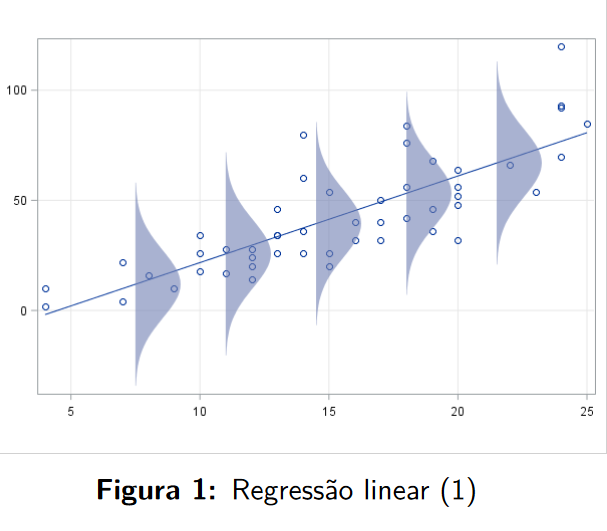
\includegraphics[width=0.5\textwidth,height=\textheight]{2024-08-10-fig1.png}

\begin{figure}
\centering
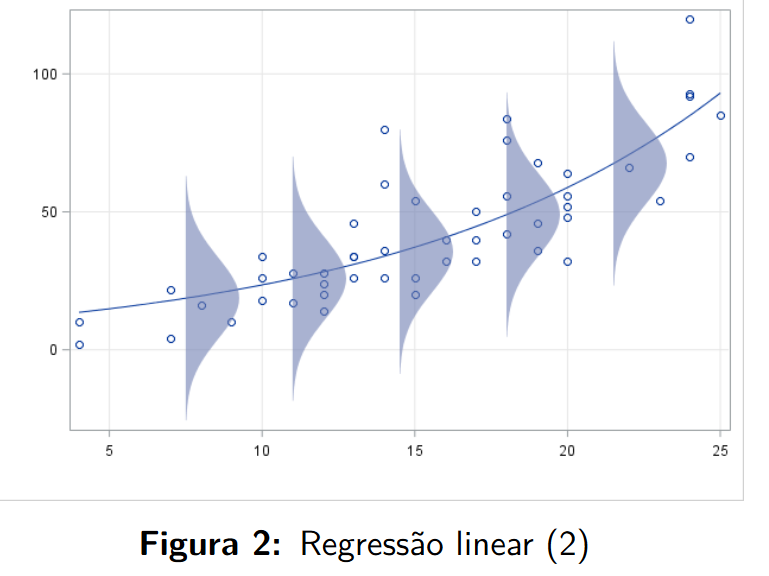
\includegraphics[width=0.5\textwidth,height=\textheight]{2024-08-10-fig2.png}
\caption{Fig 02}
\end{figure}

\begin{figure}
\centering
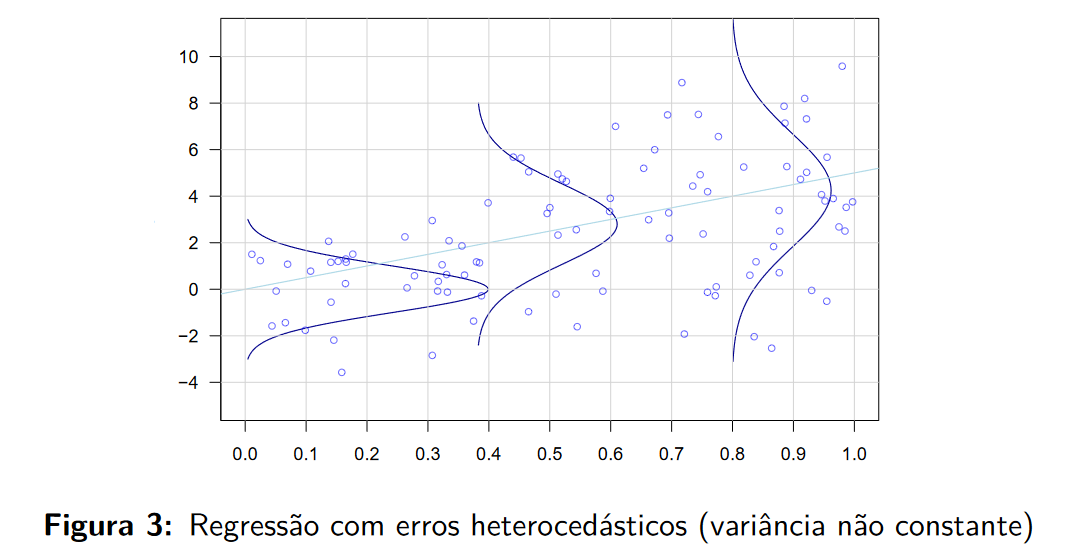
\includegraphics[width=0.5\textwidth,height=\textheight]{2024-08-10-fig3.png}
\caption{Fig 03}
\end{figure}

\begin{figure}
\centering
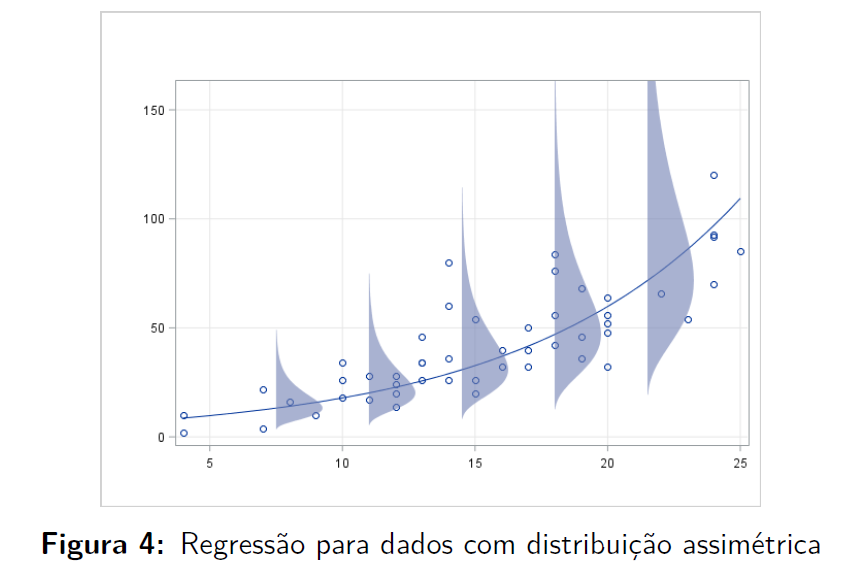
\includegraphics[width=0.5\textwidth,height=\textheight]{2024-08-10-fig4.png}
\caption{Fig 04}
\end{figure}

\begin{figure}
\centering
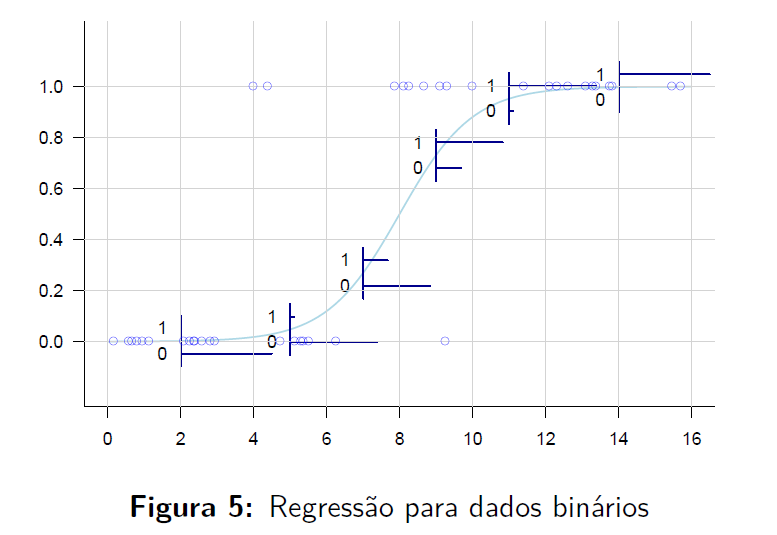
\includegraphics[width=0.5\textwidth,height=\textheight]{2024-08-10-fig5.png}
\caption{Fig 05}
\end{figure}

\begin{figure}
\centering
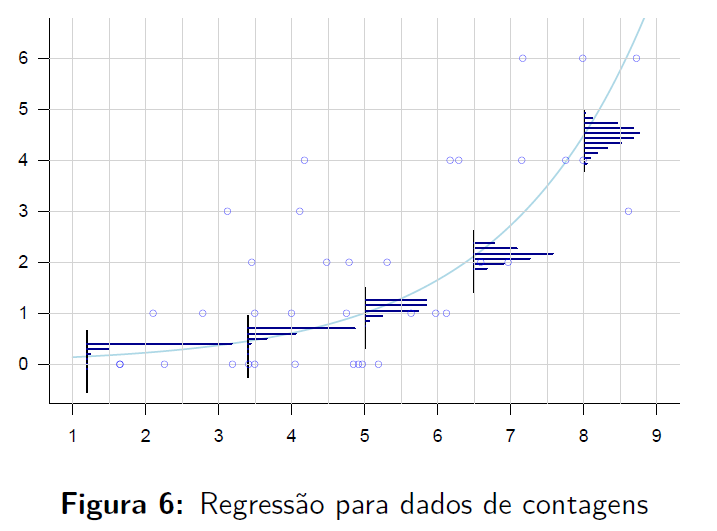
\includegraphics[width=0.5\textwidth,height=\textheight]{2024-08-10-fig6.png}
\caption{Fig 06}
\end{figure}

\subsection{Um breve histórico}\label{um-breve-histuxf3rico}

\begin{itemize}
\tightlist
\item
  Século 19: Desenvolvimento da teoria de mínimos quadrados, que serve
  de base para o ajuste de modelos de regressão.
\item
  A teoria de mínimos quadrados teve origem na Física motivada, dentre
  outros, por problemas na área navegação (século 18).
\item
  Ao longo do século 19, modelos lineares e o método de mínimos
  quadrados passaram a ser utilizados em outras ciências, baseados em
  modelos pré-estabelecidos, ou apenas em evidências empíricas.
\item
  O termo regressão foi introduzido por Francis Galton em 1875, baseado
  no princípio da ``regressão à média''.
\end{itemize}

\subsection{Regressão linear}\label{regressuxe3o-linear-1}

\begin{itemize}
\tightlist
\item
  Os dois objetivos principais de uma análise de regressão são os
  seguintes:

  \begin{itemize}
  \tightlist
  \item
    Exploratório- Analisar a relação funcional entre uma variável
    aleatória (resposta) e um conjunto de variáveis preditoras.
  \item
    Preditivo- Predizer valores não observados da variável resposta para
    valores especificados das variáveis preditoras.
  \end{itemize}
\end{itemize}

\subsection{Exemplo- Consumo de
combustível}\label{exemplo--consumo-de-combustuxedvel}

\begin{itemize}
\tightlist
\item
  Neste exemplo vamos analisar os dados da base Auto, disponíveis na
  biblioteca ISLR do R.
\item
  A base de dados dispõe de informações técnicas de 392 modelos de
  automóveis das décadas de 1970 e 1980, como consumo de combustível.
  potência do motor, dimensões dentre outras.
\item
  O objetivo aqui é ajustar modelos de regressão linear que expliquem o
  consumo de combustível com base em características do modelo.
\item
  Neste primeiro momento, para fins ilustrativos vamos considerar apenas
  duas variáveis de cada vez, embora o mais usual seja considerar
  múltiplas variáveis conjuntamente numa análise de regressão.
\end{itemize}

\begin{Shaded}
\begin{Highlighting}[]
\FunctionTok{summary}\NormalTok{(Auto)}
\end{Highlighting}
\end{Shaded}

\begin{verbatim}
##       mpg          cylinders      displacement     horsepower        weight    
##  Min.   : 9.00   Min.   :3.000   Min.   : 68.0   Min.   : 46.0   Min.   :1613  
##  1st Qu.:17.00   1st Qu.:4.000   1st Qu.:105.0   1st Qu.: 75.0   1st Qu.:2225  
##  Median :22.75   Median :4.000   Median :151.0   Median : 93.5   Median :2804  
##  Mean   :23.45   Mean   :5.472   Mean   :194.4   Mean   :104.5   Mean   :2978  
##  3rd Qu.:29.00   3rd Qu.:8.000   3rd Qu.:275.8   3rd Qu.:126.0   3rd Qu.:3615  
##  Max.   :46.60   Max.   :8.000   Max.   :455.0   Max.   :230.0   Max.   :5140  
##                                                                                
##   acceleration        year           origin                      name    
##  Min.   : 8.00   Min.   :70.00   Min.   :1.000   amc matador       :  5  
##  1st Qu.:13.78   1st Qu.:73.00   1st Qu.:1.000   ford pinto        :  5  
##  Median :15.50   Median :76.00   Median :1.000   toyota corolla    :  5  
##  Mean   :15.54   Mean   :75.98   Mean   :1.577   amc gremlin       :  4  
##  3rd Qu.:17.02   3rd Qu.:79.00   3rd Qu.:2.000   amc hornet        :  4  
##  Max.   :24.80   Max.   :82.00   Max.   :3.000   chevrolet chevette:  4  
##                                                  (Other)           :365
\end{verbatim}

\begin{Shaded}
\begin{Highlighting}[]
\FunctionTok{ggplot}\NormalTok{(Auto, }\FunctionTok{aes}\NormalTok{(}\AttributeTok{x =}\NormalTok{ year)) }\SpecialCharTok{+} \FunctionTok{geom\_histogram}\NormalTok{()}
\end{Highlighting}
\end{Shaded}

\begin{verbatim}
## `stat_bin()` using `bins = 30`. Pick better value with `binwidth`.
\end{verbatim}

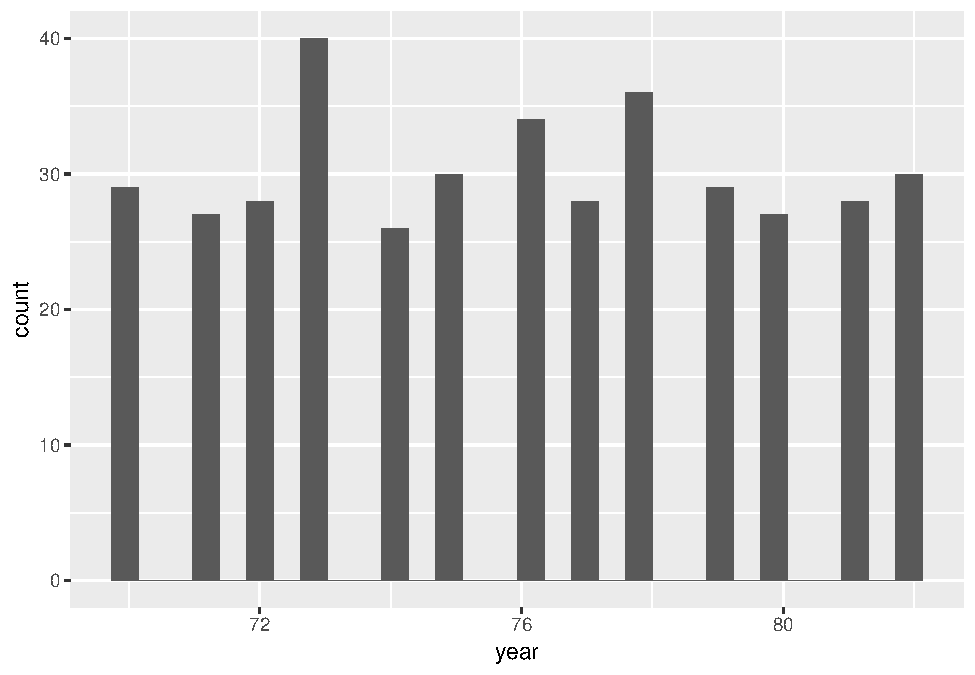
\includegraphics{Modelos_Estatisticos-2024-08-10_files/figure-latex/unnamed-chunk-3-1.pdf}

\begin{Shaded}
\begin{Highlighting}[]
\FunctionTok{ggplot}\NormalTok{(Auto, }\FunctionTok{aes}\NormalTok{(}\AttributeTok{x =}\NormalTok{ year, }\AttributeTok{y =}\NormalTok{ mpg)) }\SpecialCharTok{+} \FunctionTok{geom\_point}\NormalTok{() }\SpecialCharTok{+}
    \FunctionTok{stat\_smooth}\NormalTok{(}\AttributeTok{method =} \StringTok{"lm"}\NormalTok{) }\SpecialCharTok{+}
    \FunctionTok{theme\_bw}\NormalTok{(}\AttributeTok{base\_size =} \DecValTok{14}\NormalTok{)}
\end{Highlighting}
\end{Shaded}

\begin{verbatim}
## `geom_smooth()` using formula = 'y ~ x'
\end{verbatim}

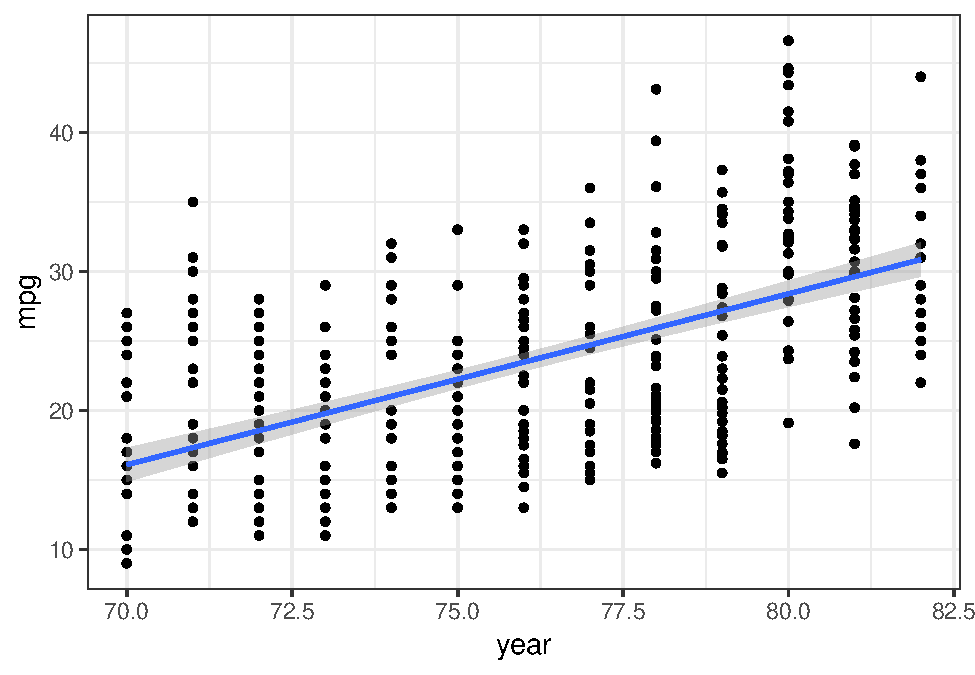
\includegraphics{Modelos_Estatisticos-2024-08-10_files/figure-latex/unnamed-chunk-3-2.pdf}

\begin{Shaded}
\begin{Highlighting}[]
\NormalTok{plot1 }\OtherTok{\textless{}{-}} \FunctionTok{ggplot}\NormalTok{(Auto, }\FunctionTok{aes}\NormalTok{(}\AttributeTok{x =}\NormalTok{ horsepower, }\AttributeTok{y =}\NormalTok{ mpg)) }\SpecialCharTok{+} \FunctionTok{geom\_point}\NormalTok{() }\SpecialCharTok{+} \FunctionTok{theme\_bw}\NormalTok{(}\AttributeTok{base\_size =} \DecValTok{14}\NormalTok{)}
\NormalTok{plot1}
\end{Highlighting}
\end{Shaded}

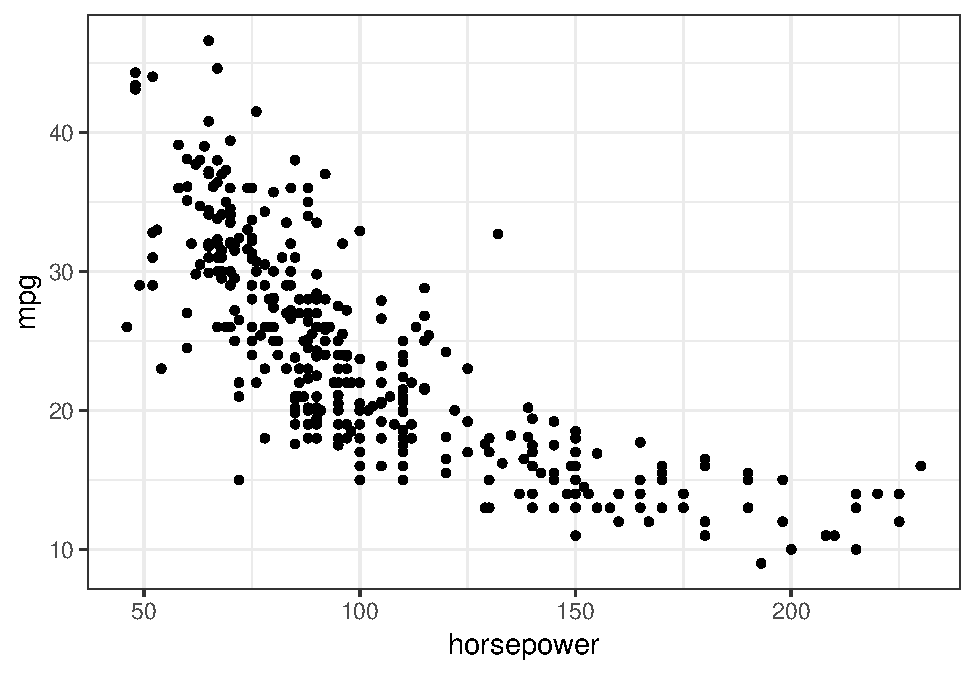
\includegraphics{Modelos_Estatisticos-2024-08-10_files/figure-latex/unnamed-chunk-4-1.pdf}

\begin{Shaded}
\begin{Highlighting}[]
\NormalTok{plot1 }\SpecialCharTok{+} \FunctionTok{coord\_trans}\NormalTok{(}\AttributeTok{x=}\StringTok{"log2"}\NormalTok{, }\AttributeTok{y=}\StringTok{"log2"}\NormalTok{)}
\end{Highlighting}
\end{Shaded}

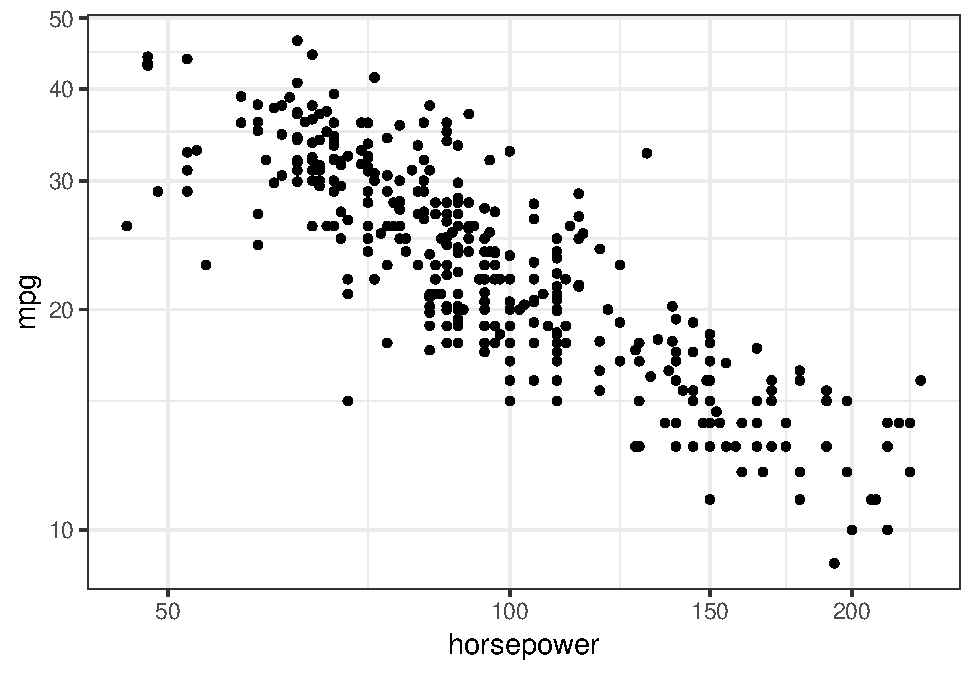
\includegraphics{Modelos_Estatisticos-2024-08-10_files/figure-latex/unnamed-chunk-4-2.pdf}

\begin{figure}
\centering
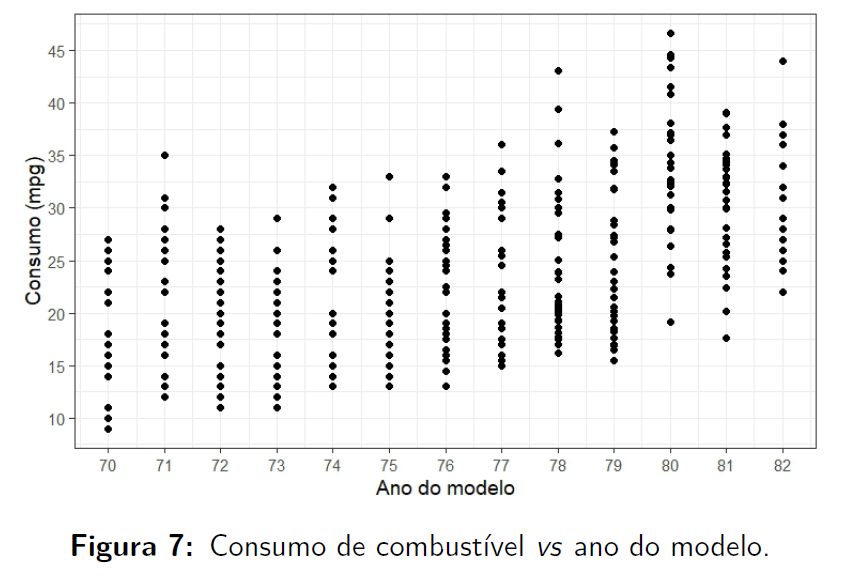
\includegraphics[width=0.5\textwidth,height=\textheight]{2024-08-10-fig7.png}
\caption{Fig 07}
\end{figure}

\begin{itemize}
\item
  Inicialmente, vamos ajustar um modelo de regressão linear que permita
  explicar o consumo de combustível (mpg- variável resposta) em função
  do ano de lançamento do modelo (yearvariável explicativa).
\item
  A Figura 7 sugere relação linear crescente entre o consumo de
  combustível e o ano de lançamento do modelo.
\item
  O modelo de regressão linear para esse par de variáveis fica
  especificado por: \[
  mpg = \beta_0 + \beta_1 \times year + \epsilon,
  \] onde \(\beta_0\) e \(\beta_1\) são os parâmetros do modelo
  (intercepto e inclinação da reta de regressão) e \(\epsilon\)
  representa os erros aleatórios.
\item
  O ajuste da regressão linear consiste na estimação dos parâmetros do
  modelo (β0 e β1), com base nos dados amostrais, que produzem a reta de
  regressão que melhor se ajusta aos dados.
\item
  O método usual de estimação dos parâmetros de uma regressão linear é o
  método de mínimos quadrados, que será estudado adiante.
\item
  Aplicando o método de mínimos quadrados, obtemos os parâmetros
  estimados \(\hat{\beta_0} = −70.01\) e \(\hat{\beta_1} = 1.23\),
  produzindo a seguinte reta de regressão ajustada: \[
  \hat{mpg} = −70.01 + 1.23 \times year
  \]
\end{itemize}

\begin{figure}
\centering
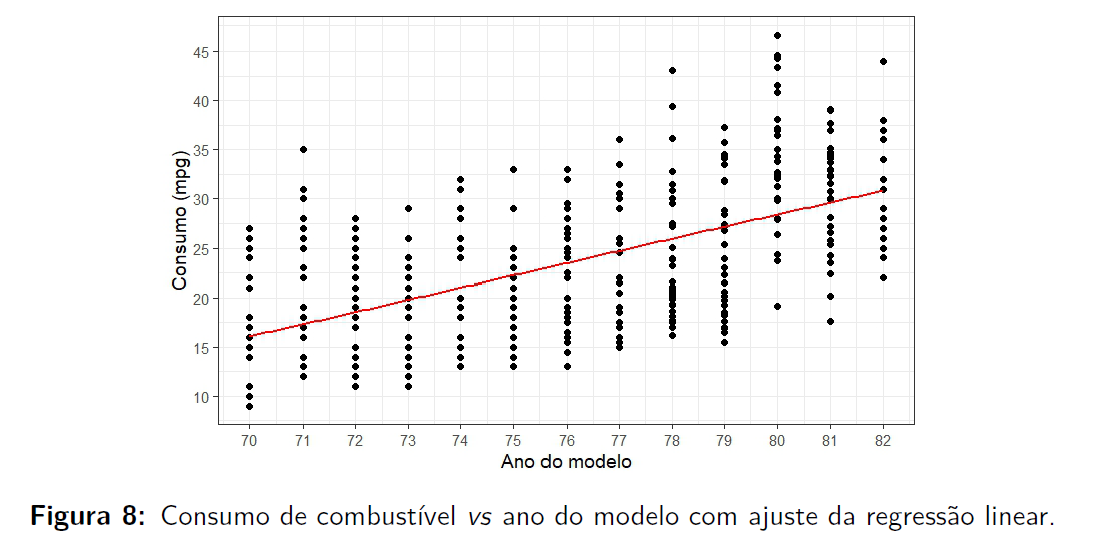
\includegraphics[width=0.5\textwidth,height=\textheight]{2024-08-10-fig8.png}
\caption{Fig 08}
\end{figure}

\begin{figure}
\centering
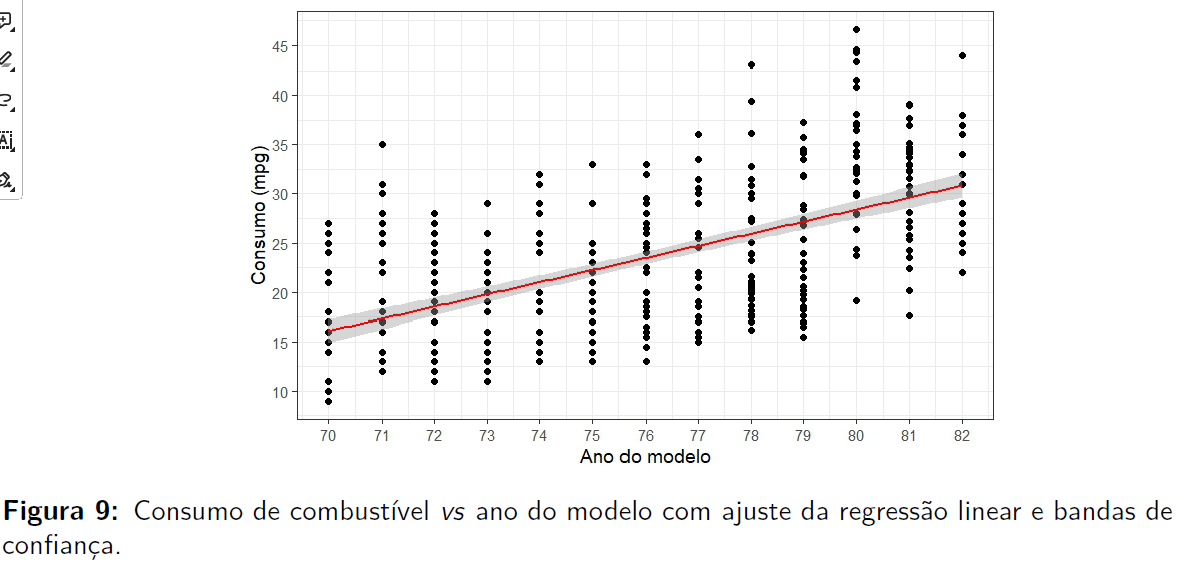
\includegraphics[width=0.5\textwidth,height=\textheight]{2024-08-10-fig9.png}
\caption{Fig 09}
\end{figure}

{[}continua\ldots.{]}

\subsection{Exemplo prático- Taxa de
formados}\label{exemplo-pruxe1tico--taxa-de-formados}

\begin{itemize}
\tightlist
\item
  Na parte prática desta aula vamos analisar dados sobre a taxa de
  formados em \(n=777\) universidades norte-americanas no ano de 1995.
\item
  O objetivo é ajustar um modelo de regressão linear que permita
  explicar a taxa de alunos formados em função das características das
  universidades e de seus alunos.
\item
  Uma breve descrição das variáveis explicativas é apresentada na
  sequência.
\end{itemize}

\subsubsection{Variaveis}\label{variaveis}

\begin{itemize}
\tightlist
\item
  \texttt{Grad.Rate}: Taxa de alunos formados (resposta);
\item
  \texttt{Apps}: Número de alunos inscritos;
\item
  \texttt{Accept}: Número de alunos aceitos;
\item
  \texttt{Enroll}: Número de novos alunos matriculados;
\item
  \texttt{Top10perc}: Percentual de novos estudantes entre os 10\%
  melhores no ensino médio;
\item
  \texttt{Top25perc}: Percentual de novos estudantes entre os 25\%
  melhores no ensino médio;
\item
  \texttt{F.Undergrad}: Número de alunos em período integral nos cursos
  de graduação;
\item
  \texttt{P.Undergrad}: Número de alunos em período parcial nos cursos
  de graduação;
\item
  \texttt{Outstate}: Número de alunos bolsistas de outros estados;
\item
  \texttt{Room.Board}: Gastos de hospedagem e alimentação;
\item
  \texttt{Books}: Gastos com materiais bibliográficos;
\item
  \texttt{Personal}: Gastos com recursos humanos;
\item
  \texttt{PhD}: Percentual de professores com doutorado;
\item
  \texttt{Terminal}: Percentual de professores com grau terminal;
\item
  \texttt{S.F.Ratio}: Razão alunos/professor;
\item
  \texttt{perc.alumni}: Percentual de ex-alunos que contribuem com
  donativos;
\item
  \texttt{Expend}: Gasto educacional por aluno.
\item
  Privada ou publica
\end{itemize}

\subsection{CODIGO}\label{codigo}

\begin{Shaded}
\begin{Highlighting}[]
\DocumentationTok{\#\#\# Carregamento e visualização inicial da base}

\FunctionTok{data}\NormalTok{(}\StringTok{"College"}\NormalTok{) }\DocumentationTok{\#\#\# Carregando a base}
\CommentTok{\#help("College") }\AlertTok{\#\#\#}\CommentTok{ Acessando a documentação}

\FunctionTok{head}\NormalTok{(College,}\DecValTok{10}\NormalTok{) }\DocumentationTok{\#\#\# Visualizando as dez primeiras linhas}
\end{Highlighting}
\end{Shaded}

\begin{verbatim}
##                              Private Apps Accept Enroll Top10perc Top25perc
## Abilene Christian University     Yes 1660   1232    721        23        52
## Adelphi University               Yes 2186   1924    512        16        29
## Adrian College                   Yes 1428   1097    336        22        50
## Agnes Scott College              Yes  417    349    137        60        89
## Alaska Pacific University        Yes  193    146     55        16        44
## Albertson College                Yes  587    479    158        38        62
## Albertus Magnus College          Yes  353    340    103        17        45
## Albion College                   Yes 1899   1720    489        37        68
## Albright College                 Yes 1038    839    227        30        63
## Alderson-Broaddus College        Yes  582    498    172        21        44
##                              F.Undergrad P.Undergrad Outstate Room.Board Books
## Abilene Christian University        2885         537     7440       3300   450
## Adelphi University                  2683        1227    12280       6450   750
## Adrian College                      1036          99    11250       3750   400
## Agnes Scott College                  510          63    12960       5450   450
## Alaska Pacific University            249         869     7560       4120   800
## Albertson College                    678          41    13500       3335   500
## Albertus Magnus College              416         230    13290       5720   500
## Albion College                      1594          32    13868       4826   450
## Albright College                     973         306    15595       4400   300
## Alderson-Broaddus College            799          78    10468       3380   660
##                              Personal PhD Terminal S.F.Ratio perc.alumni Expend
## Abilene Christian University     2200  70       78      18.1          12   7041
## Adelphi University               1500  29       30      12.2          16  10527
## Adrian College                   1165  53       66      12.9          30   8735
## Agnes Scott College               875  92       97       7.7          37  19016
## Alaska Pacific University        1500  76       72      11.9           2  10922
## Albertson College                 675  67       73       9.4          11   9727
## Albertus Magnus College          1500  90       93      11.5          26   8861
## Albion College                    850  89      100      13.7          37  11487
## Albright College                  500  79       84      11.3          23  11644
## Alderson-Broaddus College        1800  40       41      11.5          15   8991
##                              Grad.Rate
## Abilene Christian University        60
## Adelphi University                  56
## Adrian College                      54
## Agnes Scott College                 59
## Alaska Pacific University           15
## Albertson College                   55
## Albertus Magnus College             63
## Albion College                      73
## Albright College                    80
## Alderson-Broaddus College           52
\end{verbatim}

\begin{Shaded}
\begin{Highlighting}[]
\FunctionTok{dim}\NormalTok{(College) }\DocumentationTok{\#\#\# Acessando a dimensão da base}
\end{Highlighting}
\end{Shaded}

\begin{verbatim}
## [1] 777  18
\end{verbatim}

\begin{Shaded}
\begin{Highlighting}[]
\FunctionTok{summary}\NormalTok{(College) }\DocumentationTok{\#\#\# Resumo das variáveis}
\end{Highlighting}
\end{Shaded}

\begin{verbatim}
##  Private        Apps           Accept          Enroll       Top10perc    
##  No :212   Min.   :   81   Min.   :   72   Min.   :  35   Min.   : 1.00  
##  Yes:565   1st Qu.:  776   1st Qu.:  604   1st Qu.: 242   1st Qu.:15.00  
##            Median : 1558   Median : 1110   Median : 434   Median :23.00  
##            Mean   : 3002   Mean   : 2019   Mean   : 780   Mean   :27.56  
##            3rd Qu.: 3624   3rd Qu.: 2424   3rd Qu.: 902   3rd Qu.:35.00  
##            Max.   :48094   Max.   :26330   Max.   :6392   Max.   :96.00  
##    Top25perc      F.Undergrad     P.Undergrad         Outstate    
##  Min.   :  9.0   Min.   :  139   Min.   :    1.0   Min.   : 2340  
##  1st Qu.: 41.0   1st Qu.:  992   1st Qu.:   95.0   1st Qu.: 7320  
##  Median : 54.0   Median : 1707   Median :  353.0   Median : 9990  
##  Mean   : 55.8   Mean   : 3700   Mean   :  855.3   Mean   :10441  
##  3rd Qu.: 69.0   3rd Qu.: 4005   3rd Qu.:  967.0   3rd Qu.:12925  
##  Max.   :100.0   Max.   :31643   Max.   :21836.0   Max.   :21700  
##    Room.Board       Books           Personal         PhD        
##  Min.   :1780   Min.   :  96.0   Min.   : 250   Min.   :  8.00  
##  1st Qu.:3597   1st Qu.: 470.0   1st Qu.: 850   1st Qu.: 62.00  
##  Median :4200   Median : 500.0   Median :1200   Median : 75.00  
##  Mean   :4358   Mean   : 549.4   Mean   :1341   Mean   : 72.66  
##  3rd Qu.:5050   3rd Qu.: 600.0   3rd Qu.:1700   3rd Qu.: 85.00  
##  Max.   :8124   Max.   :2340.0   Max.   :6800   Max.   :103.00  
##     Terminal       S.F.Ratio      perc.alumni        Expend     
##  Min.   : 24.0   Min.   : 2.50   Min.   : 0.00   Min.   : 3186  
##  1st Qu.: 71.0   1st Qu.:11.50   1st Qu.:13.00   1st Qu.: 6751  
##  Median : 82.0   Median :13.60   Median :21.00   Median : 8377  
##  Mean   : 79.7   Mean   :14.09   Mean   :22.74   Mean   : 9660  
##  3rd Qu.: 92.0   3rd Qu.:16.50   3rd Qu.:31.00   3rd Qu.:10830  
##  Max.   :100.0   Max.   :39.80   Max.   :64.00   Max.   :56233  
##    Grad.Rate     
##  Min.   : 10.00  
##  1st Qu.: 53.00  
##  Median : 65.00  
##  Mean   : 65.46  
##  3rd Qu.: 78.00  
##  Max.   :118.00
\end{verbatim}

\begin{Shaded}
\begin{Highlighting}[]
\DocumentationTok{\#\#\# Vamos considerar Grad.Rate (taxa de formados) como a variável resposta na nossa análise. Começamos a análise com alguns gráficos.}

\FunctionTok{ggplot}\NormalTok{(College, }\FunctionTok{aes}\NormalTok{(}\AttributeTok{x =}\NormalTok{ Grad.Rate)) }\SpecialCharTok{+} \FunctionTok{geom\_histogram}\NormalTok{() }\SpecialCharTok{+}
    \FunctionTok{theme\_bw}\NormalTok{(}\AttributeTok{base\_size =} \DecValTok{14}\NormalTok{)}
\end{Highlighting}
\end{Shaded}

\begin{verbatim}
## `stat_bin()` using `bins = 30`. Pick better value with `binwidth`.
\end{verbatim}

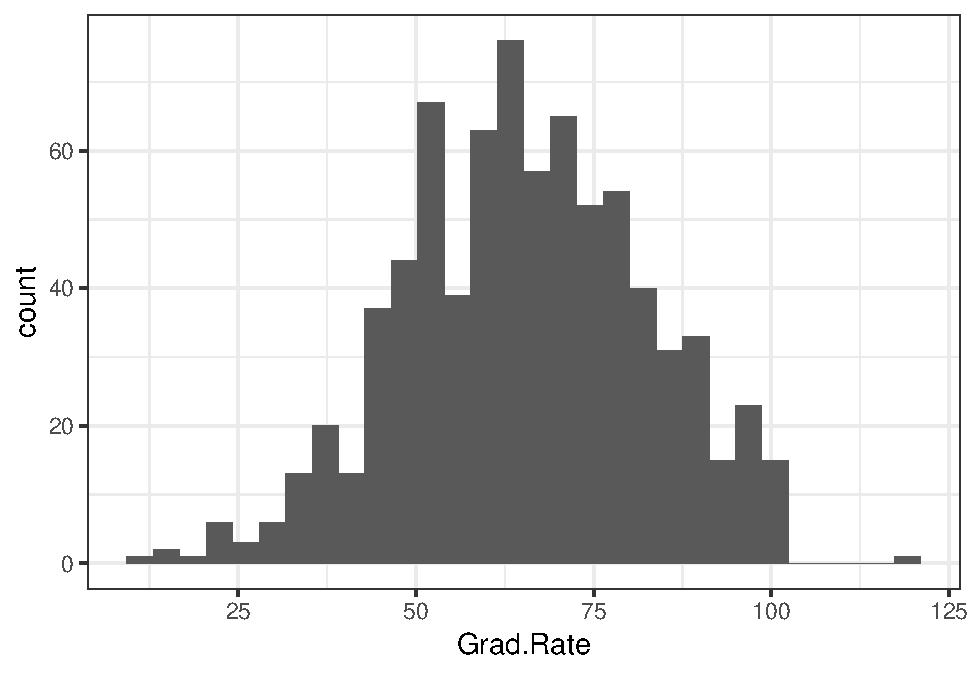
\includegraphics{Modelos_Estatisticos-2024-08-10_files/figure-latex/unnamed-chunk-6-1.pdf}

\begin{Shaded}
\begin{Highlighting}[]
\DocumentationTok{\#\#\# Distribuição das taxas de formados}

\FunctionTok{ggplot}\NormalTok{(College, }\FunctionTok{aes}\NormalTok{(}\AttributeTok{x =}\NormalTok{ Top10perc, }\AttributeTok{y =}\NormalTok{ Grad.Rate)) }\SpecialCharTok{+} \FunctionTok{geom\_point}\NormalTok{() }\SpecialCharTok{+}
    \FunctionTok{geom\_smooth}\NormalTok{(}\AttributeTok{method =} \StringTok{"loess"}\NormalTok{) }\SpecialCharTok{+} 
    \FunctionTok{theme\_bw}\NormalTok{(}\AttributeTok{base\_size =} \DecValTok{14}\NormalTok{)}
\end{Highlighting}
\end{Shaded}

\begin{verbatim}
## `geom_smooth()` using formula = 'y ~ x'
\end{verbatim}

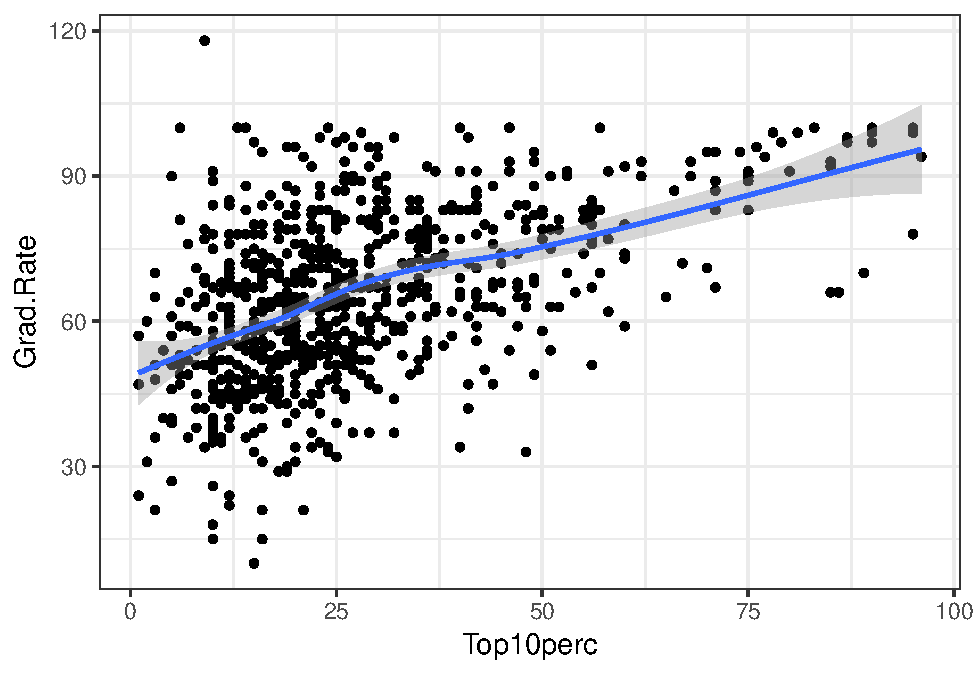
\includegraphics{Modelos_Estatisticos-2024-08-10_files/figure-latex/unnamed-chunk-6-2.pdf}

\begin{Shaded}
\begin{Highlighting}[]
\DocumentationTok{\#\#\# Taxas de formados versus percentual de alunos entre os 10\% melhores}
\DocumentationTok{\#\#\# no ensino médio.}

\FunctionTok{ggplot}\NormalTok{(College, }\FunctionTok{aes}\NormalTok{(}\AttributeTok{x =}\NormalTok{ Outstate, }\AttributeTok{y =}\NormalTok{ Grad.Rate)) }\SpecialCharTok{+} \FunctionTok{geom\_point}\NormalTok{() }\SpecialCharTok{+}
    \FunctionTok{geom\_smooth}\NormalTok{(}\AttributeTok{method =} \StringTok{"loess"}\NormalTok{) }\SpecialCharTok{+} 
    \FunctionTok{theme\_bw}\NormalTok{(}\AttributeTok{base\_size =} \DecValTok{14}\NormalTok{)}
\end{Highlighting}
\end{Shaded}

\begin{verbatim}
## `geom_smooth()` using formula = 'y ~ x'
\end{verbatim}

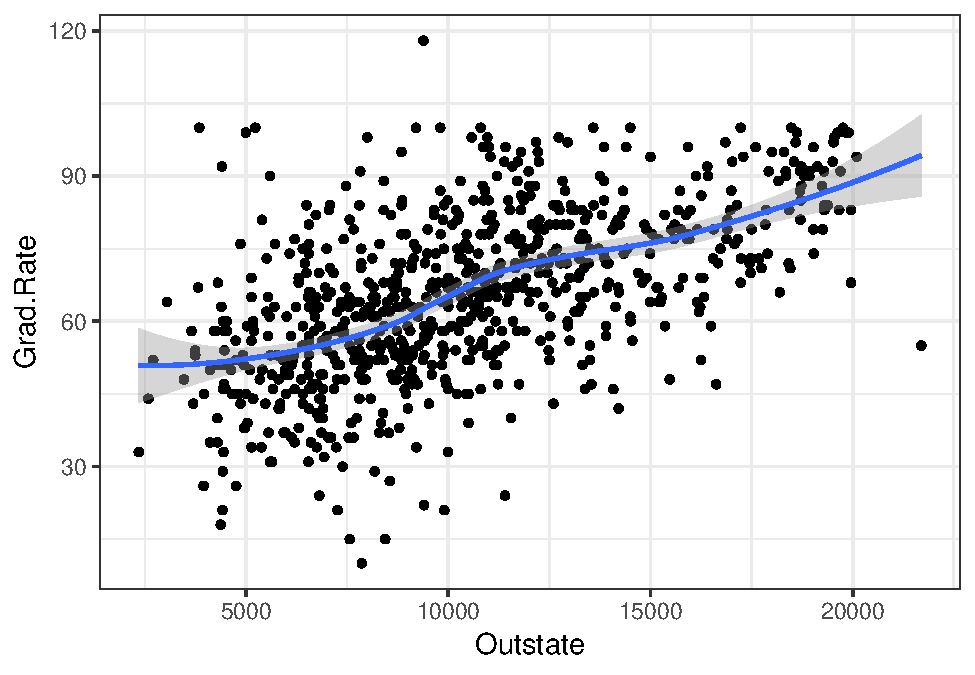
\includegraphics{Modelos_Estatisticos-2024-08-10_files/figure-latex/unnamed-chunk-6-3.pdf}

\begin{Shaded}
\begin{Highlighting}[]
\DocumentationTok{\#\#\# Taxas de formados versus investimentos externos.}

\FunctionTok{ggplot}\NormalTok{(College, }\FunctionTok{aes}\NormalTok{(}\AttributeTok{x =}\NormalTok{ perc.alumni, }\AttributeTok{y =}\NormalTok{ Grad.Rate)) }\SpecialCharTok{+} \FunctionTok{geom\_point}\NormalTok{() }\SpecialCharTok{+}
    \FunctionTok{geom\_smooth}\NormalTok{(}\AttributeTok{method =} \StringTok{"loess"}\NormalTok{) }\SpecialCharTok{+}
    \FunctionTok{theme\_bw}\NormalTok{(}\AttributeTok{base\_size =} \DecValTok{14}\NormalTok{)}
\end{Highlighting}
\end{Shaded}

\begin{verbatim}
## `geom_smooth()` using formula = 'y ~ x'
\end{verbatim}

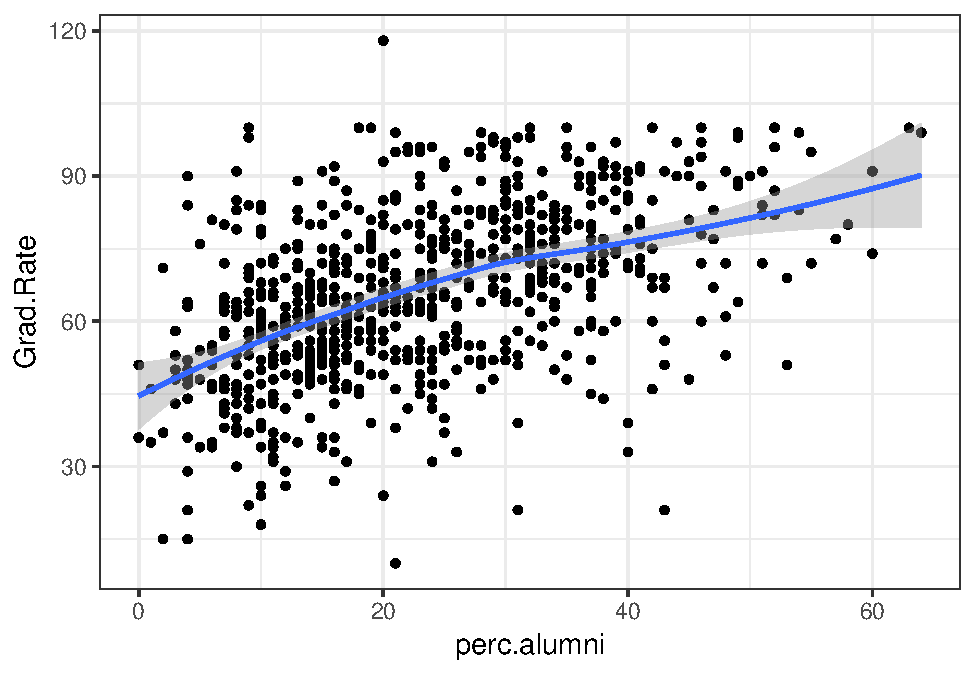
\includegraphics{Modelos_Estatisticos-2024-08-10_files/figure-latex/unnamed-chunk-6-4.pdf}

\begin{Shaded}
\begin{Highlighting}[]
\DocumentationTok{\#\#\# Taxas de formados versus porcentagens de ex{-}alunos contribuintes.}
\end{Highlighting}
\end{Shaded}

\begin{Shaded}
\begin{Highlighting}[]
\FunctionTok{ggpairs}\NormalTok{(College, }\AttributeTok{proportions =} \StringTok{"auto"}\NormalTok{) }\DocumentationTok{\#\#\# Matriz de gráficos de dispersão. {-} DEMORA PARA RODAR}

\CommentTok{\#para salvar o ultimo grafico}
\FunctionTok{ggsave}\NormalTok{(}\StringTok{"plot\_grande.png"}\NormalTok{, }\AttributeTok{device =} \StringTok{"png"}\NormalTok{, }\AttributeTok{width =} \DecValTok{100}\NormalTok{, }\AttributeTok{height =} \DecValTok{80}\NormalTok{, }\AttributeTok{units =} \StringTok{"cm"}\NormalTok{)}
\CommentTok{\# tamanho maximo 50 in ou 126 cm}
\end{Highlighting}
\end{Shaded}

\begin{figure}
\centering
\includegraphics[width=1\textwidth,height=\textheight]{plot_grande.png}
\caption{Grafico pesado}
\end{figure}

\begin{Shaded}
\begin{Highlighting}[]
\FunctionTok{ggcorr}\NormalTok{(College[,}\SpecialCharTok{{-}}\DecValTok{1}\NormalTok{], }\AttributeTok{label =} \ConstantTok{TRUE}\NormalTok{, }\AttributeTok{label\_round =} \DecValTok{2}\NormalTok{) }\DocumentationTok{\#\#\# Correlograma.}
\FunctionTok{ggsave}\NormalTok{(}\StringTok{"plot\_colorido.png"}\NormalTok{, }\AttributeTok{device =} \StringTok{"png"}\NormalTok{, }\AttributeTok{width =} \DecValTok{30}\NormalTok{, }\AttributeTok{height =} \DecValTok{20}\NormalTok{, }\AttributeTok{units =} \StringTok{"cm"}\NormalTok{)}
\end{Highlighting}
\end{Shaded}

\begin{figure}
\centering
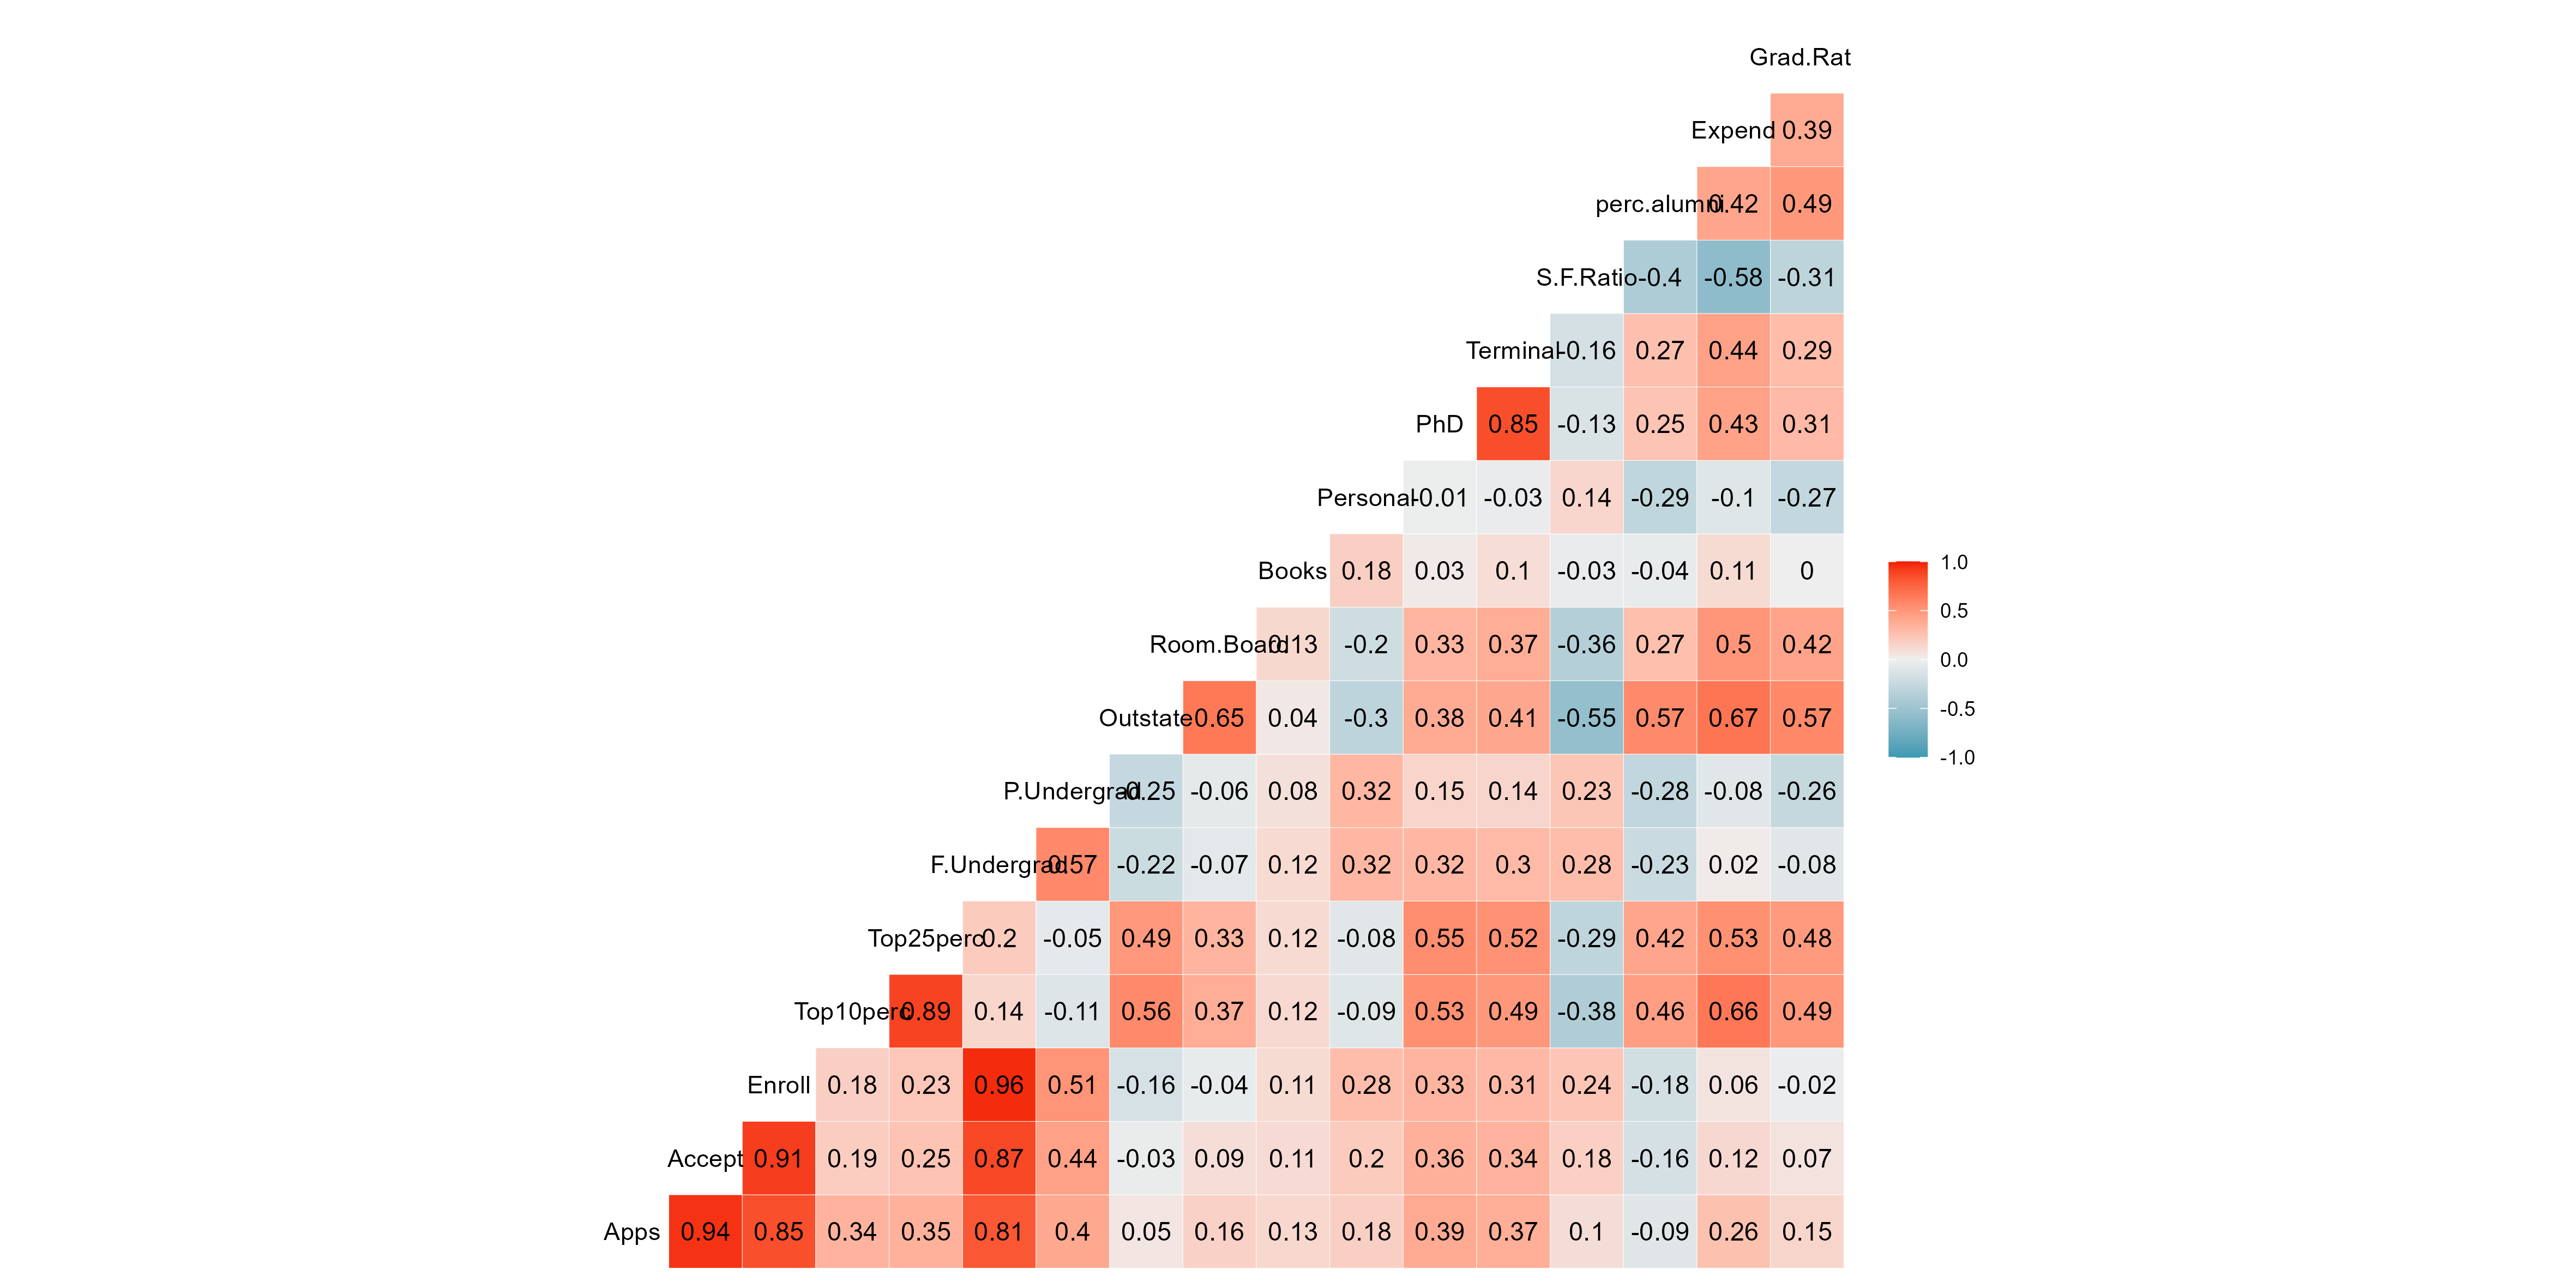
\includegraphics[width=1\textwidth,height=\textheight]{plot_colorido.png}
\caption{Grafico colorido}
\end{figure}

\begin{Shaded}
\begin{Highlighting}[]
\DocumentationTok{\#\#\# Parte 1 {-} Ajuste dos modelos lineares. Comecemos com o caso de apenas uma }
\DocumentationTok{\#\#\# variável explicativa (no caso, perc.alumni)}

\DocumentationTok{\#\#\# Para ajustar modelos lineares no R usamos a função lm. Vamos consultar}
\DocumentationTok{\#\#\# a documentação da função.}

\CommentTok{\#help(\textquotesingle{}lm\textquotesingle{})}
\end{Highlighting}
\end{Shaded}

Multipla (1 var resposta) e Multivarida (mais var respostas) são coisas
diferentes

\begin{Shaded}
\begin{Highlighting}[]
\DocumentationTok{\#\#\# Ajuste da regressão linear simples (assumindo relação linear entre a taxa de formados e o percentual de ex{-}alunos contribuintes)}

\NormalTok{ajuste1 }\OtherTok{\textless{}{-}} \FunctionTok{lm}\NormalTok{(Grad.Rate }\SpecialCharTok{\textasciitilde{}}\NormalTok{ perc.alumni, }\AttributeTok{data =}\NormalTok{ College) }\DocumentationTok{\#\#\#(resposta \textasciitilde{} var.explicativas)}

\NormalTok{ajuste1}
\end{Highlighting}
\end{Shaded}

\begin{verbatim}
## 
## Call:
## lm(formula = Grad.Rate ~ perc.alumni, data = College)
## 
## Coefficients:
## (Intercept)  perc.alumni  
##     49.9863       0.6805
\end{verbatim}

\[
\hat{Grad.Rate} = 49,9863 + 0,6805 \times perc.alumni
\] chapeu indica estimado?

\begin{Shaded}
\begin{Highlighting}[]
\FunctionTok{summary}\NormalTok{(ajuste1)}
\end{Highlighting}
\end{Shaded}

\begin{verbatim}
## 
## Call:
## lm(formula = Grad.Rate ~ perc.alumni, data = College)
## 
## Residuals:
##     Min      1Q  Median      3Q     Max 
## -58.247  -9.513   0.043   9.362  54.404 
## 
## Coefficients:
##             Estimate Std. Error t value Pr(>|t|)    
## (Intercept) 49.98633    1.12345   44.49   <2e-16 ***
## perc.alumni  0.68049    0.04338   15.69   <2e-16 ***
## ---
## Signif. codes:  0 '***' 0.001 '**' 0.01 '*' 0.05 '.' 0.1 ' ' 1
## 
## Residual standard error: 14.98 on 775 degrees of freedom
## Multiple R-squared:  0.241,  Adjusted R-squared:   0.24 
## F-statistic: 246.1 on 1 and 775 DF,  p-value: < 2.2e-16
\end{verbatim}

\begin{Shaded}
\begin{Highlighting}[]
\DocumentationTok{\#\#\# O percentual de ex{-}alunos contribuintes tem efeito positivo, e }
\DocumentationTok{\#\#\# estatisticamente significativo na taxa de formados.}
\end{Highlighting}
\end{Shaded}

\begin{Shaded}
\begin{Highlighting}[]
\DocumentationTok{\#\#\# Vamos visualizar o ajuste do modelo}
\FunctionTok{ggplot}\NormalTok{(College, }\FunctionTok{aes}\NormalTok{(}\AttributeTok{x =}\NormalTok{ perc.alumni, }\AttributeTok{y =}\NormalTok{ Grad.Rate)) }\SpecialCharTok{+} \FunctionTok{geom\_point}\NormalTok{() }\SpecialCharTok{+}
    \FunctionTok{stat\_smooth}\NormalTok{(}\AttributeTok{method =} \StringTok{"lm"}\NormalTok{) }\SpecialCharTok{+}
    \FunctionTok{theme\_bw}\NormalTok{(}\AttributeTok{base\_size =} \DecValTok{14}\NormalTok{)}
\end{Highlighting}
\end{Shaded}

\begin{verbatim}
## `geom_smooth()` using formula = 'y ~ x'
\end{verbatim}

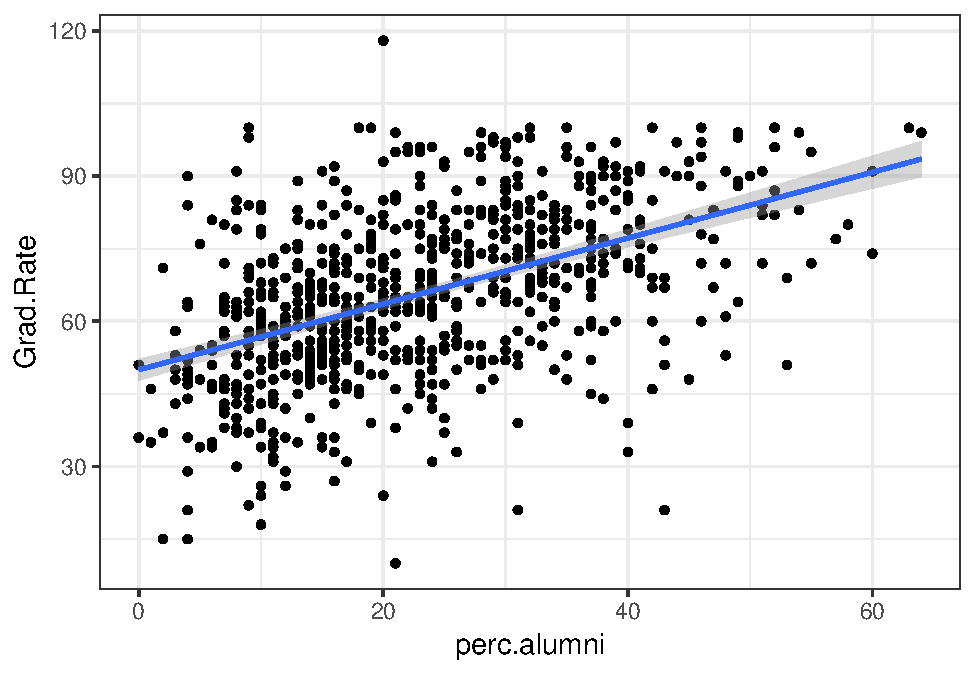
\includegraphics{Modelos_Estatisticos-2024-08-10_files/figure-latex/unnamed-chunk-13-1.pdf}

\begin{Shaded}
\begin{Highlighting}[]
\DocumentationTok{\#\#\# Vamos investigar possível efeito quadrático do percentual de contribuíntes na taxa de formados. Para isso, adicionamos ao preditor o termo quadrático da variável explicativa, da seguinte forma:}

\NormalTok{ajuste2 }\OtherTok{\textless{}{-}} \FunctionTok{lm}\NormalTok{(Grad.Rate }\SpecialCharTok{\textasciitilde{}}\NormalTok{ perc.alumni }\SpecialCharTok{+} \FunctionTok{I}\NormalTok{(perc.alumni}\SpecialCharTok{\^{}}\DecValTok{2}\NormalTok{), }\AttributeTok{data =}\NormalTok{ College)}
\FunctionTok{summary}\NormalTok{(ajuste2)}
\end{Highlighting}
\end{Shaded}

\begin{verbatim}
## 
## Call:
## lm(formula = Grad.Rate ~ perc.alumni + I(perc.alumni^2), data = College)
## 
## Residuals:
##     Min      1Q  Median      3Q     Max 
## -57.444  -9.146   0.042   9.448  53.446 
## 
## Coefficients:
##                   Estimate Std. Error t value Pr(>|t|)    
## (Intercept)      45.896244   1.877789  24.442  < 2e-16 ***
## perc.alumni       1.085948   0.155614   6.978 6.42e-12 ***
## I(perc.alumni^2) -0.007652   0.002821  -2.712  0.00683 ** 
## ---
## Signif. codes:  0 '***' 0.001 '**' 0.01 '*' 0.05 '.' 0.1 ' ' 1
## 
## Residual standard error: 14.91 on 774 degrees of freedom
## Multiple R-squared:  0.2481, Adjusted R-squared:  0.2462 
## F-statistic: 127.7 on 2 and 774 DF,  p-value: < 2.2e-16
\end{verbatim}

\begin{Shaded}
\begin{Highlighting}[]
\DocumentationTok{\#\#\# O termo quadrático é estatisticamente significativo, indicando que a}
\DocumentationTok{\#\#\# relação entre as variáveis não é linear. Vamos dar um passo além, e}
\DocumentationTok{\#\#\# incluir o termo de terceira ordem para o percentual de contribuintes}
\DocumentationTok{\#\#\# (modelo cúbico).}
\end{Highlighting}
\end{Shaded}

\[
\hat{Grad.Rate} = 45.896244 + 1.085948 \times perc.alumni -0.007652 \times perc.alumni^2
\]

de acordo com os valores de p é significativo, então manteria essa
variavel

\begin{Shaded}
\begin{Highlighting}[]
\NormalTok{ajuste22 }\OtherTok{\textless{}{-}} \FunctionTok{lm}\NormalTok{(}\AttributeTok{formula =}\NormalTok{ Grad.Rate }\SpecialCharTok{\textasciitilde{}}\NormalTok{ ., }\AttributeTok{data =}\NormalTok{ College)}
\FunctionTok{summary}\NormalTok{(ajuste22)}
\end{Highlighting}
\end{Shaded}

\begin{verbatim}
## 
## Call:
## lm(formula = Grad.Rate ~ ., data = College)
## 
## Residuals:
##     Min      1Q  Median      3Q     Max 
## -53.897  -7.132  -0.292   7.213  54.056 
## 
## Coefficients:
##               Estimate Std. Error t value Pr(>|t|)    
## (Intercept) 33.8736716  4.8480858   6.987 6.15e-12 ***
## PrivateYes   3.3813758  1.6965147   1.993 0.046605 *  
## Apps         0.0012984  0.0004418   2.939 0.003390 ** 
## Accept      -0.0006961  0.0008627  -0.807 0.419995    
## Enroll       0.0021593  0.0023081   0.936 0.349814    
## Top10perc    0.0548964  0.0717587   0.765 0.444501    
## Top25perc    0.1351288  0.0549667   2.458 0.014179 *  
## F.Undergrad -0.0004712  0.0004008  -1.176 0.240138    
## P.Undergrad -0.0014836  0.0003902  -3.802 0.000155 ***
## Outstate     0.0010174  0.0002334   4.359 1.49e-05 ***
## Room.Board   0.0019143  0.0005908   3.240 0.001246 ** 
## Books       -0.0022205  0.0029168  -0.761 0.446739    
## Personal    -0.0016635  0.0007698  -2.161 0.031000 *  
## PhD          0.0872827  0.0568102   1.536 0.124859    
## Terminal    -0.0747023  0.0623172  -1.199 0.231002    
## S.F.Ratio    0.0758222  0.1593102   0.476 0.634254    
## perc.alumni  0.2793343  0.0491750   5.680 1.91e-08 ***
## Expend      -0.0004565  0.0001542  -2.961 0.003163 ** 
## ---
## Signif. codes:  0 '***' 0.001 '**' 0.01 '*' 0.05 '.' 0.1 ' ' 1
## 
## Residual standard error: 12.75 on 759 degrees of freedom
## Multiple R-squared:  0.4615, Adjusted R-squared:  0.4495 
## F-statistic: 38.27 on 17 and 759 DF,  p-value: < 2.2e-16
\end{verbatim}

\begin{Shaded}
\begin{Highlighting}[]
\DocumentationTok{\#\# PrivateYes {-}\textgreater{} 1 se privada (YES); 0 se publica(No)}

\DocumentationTok{\#\# Nesse modelo (ajustado com todas as outras variaveis) as escolas privadas tem p\textless{}0.05, portanto ser privada tem um impacto  no (maior) número de formados (3.3 pontos percentuais)}

\NormalTok{ajuste23 }\OtherTok{\textless{}{-}} \FunctionTok{lm}\NormalTok{(}\AttributeTok{formula =}\NormalTok{ Grad.Rate }\SpecialCharTok{\textasciitilde{}}\NormalTok{ Private , }\AttributeTok{data =}\NormalTok{ College)}
\FunctionTok{summary}\NormalTok{(ajuste23)}
\end{Highlighting}
\end{Shaded}

\begin{verbatim}
## 
## Call:
## lm(formula = Grad.Rate ~ Private, data = College)
## 
## Residuals:
##     Min      1Q  Median      3Q     Max 
## -53.998 -10.042   0.002  11.002  49.002 
## 
## Coefficients:
##             Estimate Std. Error t value Pr(>|t|)    
## (Intercept)   56.042      1.112  50.406   <2e-16 ***
## PrivateYes    12.956      1.304   9.937   <2e-16 ***
## ---
## Signif. codes:  0 '***' 0.001 '**' 0.01 '*' 0.05 '.' 0.1 ' ' 1
## 
## Residual standard error: 16.19 on 775 degrees of freedom
## Multiple R-squared:  0.113,  Adjusted R-squared:  0.1119 
## F-statistic: 98.74 on 1 and 775 DF,  p-value: < 2.2e-16
\end{verbatim}

\begin{Shaded}
\begin{Highlighting}[]
\DocumentationTok{\#\# Num modelo só com a privada ela (por "acaso") tambem teve p\textless{}0.05 mas com um impacto diferente (12.9 pontos percentuais)}
\end{Highlighting}
\end{Shaded}

\begin{Shaded}
\begin{Highlighting}[]
\FunctionTok{confint}\NormalTok{(ajuste22) }\DocumentationTok{\#\#\# Intervalo de confiaça}
\end{Highlighting}
\end{Shaded}

\begin{verbatim}
##                     2.5 %        97.5 %
## (Intercept) 24.3564214869 43.3909217410
## PrivateYes   0.0509572771  6.7117943696
## Apps         0.0004312157  0.0021656167
## Accept      -0.0023897796  0.0009975317
## Enroll      -0.0023717122  0.0066902689
## Top10perc   -0.0859726333  0.1957655121
## Top25perc    0.0272239131  0.2430337318
## F.Undergrad -0.0012581212  0.0003156791
## P.Undergrad -0.0022496029 -0.0007176822
## Outstate     0.0005592115  0.0014756792
## Room.Board   0.0007545476  0.0030741345
## Books       -0.0079464883  0.0035055569
## Personal    -0.0031746541 -0.0001524155
## PhD         -0.0242410359  0.1988064637
## Terminal    -0.1970367830  0.0476322483
## S.F.Ratio   -0.2369186844  0.3885630948
## perc.alumni  0.1827990643  0.3758695198
## Expend      -0.0007590979 -0.0001538281
\end{verbatim}

\[
\hat{Grad.Rate} = 33,87 + 3,38 \times (Private = Yes) + 0.0012984 \times (Apps)
\]

Variavel Dummie: (relevel)

\begin{itemize}
\item
  Sexo: F, M -\textgreater{} Sexo Feminino (1 se feminino, 0 se
  masculino)
\item
  Escolaridade: Sem\_Escolaridade, EF, EM, ES -\textgreater{}

  \begin{itemize}
  \tightlist
  \item
    EF (1 ou 0)
  \item
    EM (1 ou 0)
  \item
    ES (1 ou 0)
  \item
    Sendo 1 TEM e 0 Não tem, consequentemente os 3 zeros é
    Sem\_Escolaridade
  \end{itemize}
\end{itemize}

\[
\hat{y} = \hat{\beta_0} + \hat{\beta_1} \times EF + \hat{\beta_2} \times EM + \hat{\beta_3} \times ES
\] - Sem escolaridade: \(\hat{y} = \hat{\beta_0}\)

\begin{itemize}
\item
  Ens. Fund: \(\hat{y} = \hat{\beta_0} + \hat{\beta_1}\)
\item
  Ens. Med: \(\hat{y} = \hat{\beta_0} + \hat{\beta_2}\)
\item
  Ens. Sup: \(\hat{y} = \hat{\beta_0} + \hat{\beta_3}\)
\end{itemize}

Se for EM/EF: \[
\hat{y} = (\hat{\beta_0} + \hat{\beta_1}) - (\hat{\beta_0} + \hat{\beta_2}) = \hat{\beta_1} - \hat{\beta_2}
\]

\[
y = \beta_0 + \beta_1 x + \varepsilon
\] \[
\varepsilon = (y - (\beta_0 + \beta_1 x))
\] \[
residuo = y - (\hat{\beta_0} + \hat{ \beta_1 } x)
\] Erro é o ``real'', residuo é o estimado.

\begin{Shaded}
\begin{Highlighting}[]
\NormalTok{ajuste3 }\OtherTok{\textless{}{-}} \FunctionTok{lm}\NormalTok{(Grad.Rate }\SpecialCharTok{\textasciitilde{}}\NormalTok{ perc.alumni }\SpecialCharTok{+} \FunctionTok{I}\NormalTok{(perc.alumni}\SpecialCharTok{\^{}}\DecValTok{2}\NormalTok{) }\SpecialCharTok{+} \FunctionTok{I}\NormalTok{(perc.alumni}\SpecialCharTok{\^{}}\DecValTok{3}\NormalTok{), }\AttributeTok{data =}\NormalTok{ College)}
\FunctionTok{summary}\NormalTok{(ajuste3)}
\end{Highlighting}
\end{Shaded}

\begin{verbatim}
## 
## Call:
## lm(formula = Grad.Rate ~ perc.alumni + I(perc.alumni^2) + I(perc.alumni^3), 
##     data = College)
## 
## Residuals:
##     Min      1Q  Median      3Q     Max 
## -56.571  -9.123   0.005   9.346  52.896 
## 
## Coefficients:
##                    Estimate Std. Error t value Pr(>|t|)    
## (Intercept)      42.9519252  2.8823421  14.902  < 2e-16 ***
## perc.alumni       1.5681680  0.3905839   4.015 6.53e-05 ***
## I(perc.alumni^2) -0.0276219  0.0151030  -1.829   0.0678 .  
## I(perc.alumni^3)  0.0002297  0.0001706   1.346   0.1787    
## ---
## Signif. codes:  0 '***' 0.001 '**' 0.01 '*' 0.05 '.' 0.1 ' ' 1
## 
## Residual standard error: 14.91 on 773 degrees of freedom
## Multiple R-squared:  0.2499, Adjusted R-squared:  0.247 
## F-statistic: 85.84 on 3 and 773 DF,  p-value: < 2.2e-16
\end{verbatim}

\begin{Shaded}
\begin{Highlighting}[]
\DocumentationTok{\#\#\# O termo de ordem cúbica não tem significância estatística. Vamos seguir}
\DocumentationTok{\#\#\# a análise com o modelo quadrático.}
\end{Highlighting}
\end{Shaded}

\[
\hat{Grad.Rate} = 42.9519252 + 1.5681680 \times perc.alumni -0.0276219 \times perc.alumni^2 + 0.0002297 \times perc.alumni^3
\] de acordo com os valores de p é significativo, então manteria essa
variavel

\begin{Shaded}
\begin{Highlighting}[]
\DocumentationTok{\#\#\# Vamos extrair alguns elementos do modelo ajustado}
\NormalTok{ajuste2}\SpecialCharTok{$}\NormalTok{coefficients }\DocumentationTok{\#\#\# Estimativas dos parâmetros}
\end{Highlighting}
\end{Shaded}

\begin{verbatim}
##      (Intercept)      perc.alumni I(perc.alumni^2) 
##     45.896244242      1.085947860     -0.007651754
\end{verbatim}

\begin{Shaded}
\begin{Highlighting}[]
\NormalTok{ajuste2}\SpecialCharTok{$}\NormalTok{residuals }\DocumentationTok{\#\#\# Resíduos ordeinários, resultado muito longo, então resumido a seguir}
\end{Highlighting}
\end{Shaded}

\begin{Shaded}
\begin{Highlighting}[]
\FunctionTok{head}\NormalTok{(ajuste2}\SpecialCharTok{$}\NormalTok{residuals) }
\end{Highlighting}
\end{Shaded}

\begin{verbatim}
## Abilene Christian University           Adelphi University 
##                     2.174234                    -5.312561 
##               Adrian College          Agnes Scott College 
##                   -17.588102                   -16.601064 
##    Alaska Pacific University            Albertson College 
##                   -33.037533                    -1.915809
\end{verbatim}

\begin{Shaded}
\begin{Highlighting}[]
\FunctionTok{tail}\NormalTok{(ajuste2}\SpecialCharTok{$}\NormalTok{residuals)}
\end{Highlighting}
\end{Shaded}

\begin{verbatim}
## Worcester Polytechnic Institute         Worcester State College 
##                        8.026956                      -19.599771 
##               Xavier University  Xavier University of Louisiana 
##                       10.792707                      -15.554500 
##                 Yale University    York College of Pennsylvania 
##                       18.264171                       28.696191
\end{verbatim}

\begin{Shaded}
\begin{Highlighting}[]
\NormalTok{ajuste2}\SpecialCharTok{$}\NormalTok{fitted.values }\DocumentationTok{\#\#\# Valores ajustados pelo modelo, resultado muito longo, então resumido a seguir}
\end{Highlighting}
\end{Shaded}

\begin{Shaded}
\begin{Highlighting}[]
\FunctionTok{head}\NormalTok{(ajuste2}\SpecialCharTok{$}\NormalTok{fitted.values) }
\end{Highlighting}
\end{Shaded}

\begin{verbatim}
## Abilene Christian University           Adelphi University 
##                     57.82577                     61.31256 
##               Adrian College          Agnes Scott College 
##                     71.58810                     75.60106 
##    Alaska Pacific University            Albertson College 
##                     48.03753                     56.91581
\end{verbatim}

\begin{Shaded}
\begin{Highlighting}[]
\FunctionTok{tail}\NormalTok{(ajuste2}\SpecialCharTok{$}\NormalTok{fitted.values)}
\end{Highlighting}
\end{Shaded}

\begin{verbatim}
## Worcester Polytechnic Institute         Worcester State College 
##                        73.97304                        59.59977 
##               Xavier University  Xavier University of Louisiana 
##                        72.20729                        64.55450 
##                 Yale University    York College of Pennsylvania 
##                        80.73583                        70.30381
\end{verbatim}

\begin{Shaded}
\begin{Highlighting}[]
\FunctionTok{model.matrix}\NormalTok{(ajuste2) }\DocumentationTok{\#\#\# Matriz do modelo (matriz X)}
\end{Highlighting}
\end{Shaded}

\begin{verbatim}
##                                               (Intercept) perc.alumni
## Abilene Christian University                            1          12
## Adelphi University                                      1          16
## Adrian College                                          1          30
## Agnes Scott College                                     1          37
## Alaska Pacific University                               1           2
## Albertson College                                       1          11
## Albertus Magnus College                                 1          26
## Albion College                                          1          37
## Albright College                                        1          23
## Alderson-Broaddus College                               1          15
## Alfred University                                       1          31
## Allegheny College                                       1          41
## Allentown Coll. of St. Francis de Sales                 1          21
## Alma College                                            1          32
## Alverno College                                         1          26
## American International College                          1          19
## Amherst College                                         1          63
## Anderson University                                     1          14
## Andrews University                                      1          18
## Angelo State University                                 1           5
## Antioch University                                      1          35
## Appalachian State University                            1          14
## Aquinas College                                         1          25
## Arizona State University Main campus                    1           5
## Arkansas College (Lyon College)                         1          24
## Arkansas Tech University                                1           5
## Assumption College                                      1          30
## Auburn University-Main Campus                           1          18
## Augsburg College                                        1          31
## Augustana College IL                                    1          40
## Augustana College                                       1          30
## Austin College                                          1          33
## Averett College                                         1          11
## Baker University                                        1          21
## Baldwin-Wallace College                                 1          20
## Barat College                                           1          35
## Bard College                                            1          30
## Barnard College                                         1          33
## Barry University                                        1          11
## Baylor University                                       1          38
## Beaver College                                          1          30
## Bellarmine College                                      1          31
## Belmont Abbey College                                   1          10
## Belmont University                                      1          19
## Beloit College                                          1          26
## Bemidji State University                                1          16
## Benedictine College                                     1          18
## Bennington College                                      1          33
## Bentley College                                         1          20
## Berry College                                           1          17
## Bethany College                                         1          29
## Bethel College KS                                       1          32
## Bethel College                                          1          13
## Bethune Cookman College                                 1           9
## Birmingham-Southern College                             1          34
## Blackburn College                                       1          53
## Bloomsburg Univ. of Pennsylvania                        1          19
## Bluefield College                                       1           3
## Bluffton College                                        1          19
## Boston University                                       1          16
## Bowdoin College                                         1          52
## Bowling Green State University                          1          14
## Bradford College                                        1          21
## Bradley University                                      1          21
## Brandeis University                                     1          24
## Brenau University                                       1          12
## Brewton-Parker College                                  1          10
## Briar Cliff College                                     1          26
## Bridgewater College                                     1          24
## Brigham Young University at Provo                       1          40
## Brown University                                        1          39
## Bryn Mawr College                                       1          49
## Bucknell University                                     1          36
## Buena Vista College                                     1          10
## Butler University                                       1          29
## Cabrini College                                         1          36
## Caldwell College                                        1          25
## California Lutheran University                          1          17
## California Polytechnic-San Luis                         1          13
## California State University at Fresno                   1           8
## Calvin College                                          1          41
## Campbell University                                     1          34
## Campbellsville College                                  1          13
## Canisius College                                        1          26
## Capital University                                      1          27
## Capitol College                                         1          24
## Carleton College                                        1          60
## Carnegie Mellon University                              1          31
## Carroll College                                         1          25
## Carson-Newman College                                   1          16
## Carthage College                                        1          22
## Case Western Reserve University                         1          29
## Castleton State College                                 1           8
## Catawba College                                         1          27
## Catholic University of America                          1          18
## Cazenovia College                                       1          20
## Cedar Crest College                                     1          39
## Cedarville College                                      1          34
## Centenary College                                       1          20
## Centenary College of Louisiana                          1          25
## Center for Creative Studies                             1           4
## Central College                                         1          29
## Central Connecticut State University                    1           4
## Central Missouri State University                       1           4
## Central Washington University                           1           0
## Central Wesleyan College                                1          18
## Centre College                                          1          60
## Chapman University                                      1           6
## Chatham College                                         1          37
## Chestnut Hill College                                   1          29
## Christendom College                                     1          17
## Christian Brothers University                           1          24
## Christopher Newport University                          1          16
## Claflin College                                         1          31
## Claremont McKenna College                               1          52
## Clark University                                        1          35
## Clarke College                                          1          27
## Clarkson University                                     1          32
## Clemson University                                      1          17
## Clinch Valley Coll. of  the Univ. of Virginia           1           9
## Coe College                                             1          32
## Coker College                                           1          39
## Colby College                                           1          41
## Colgate University                                      1          45
## College Misericordia                                    1          23
## College of Charleston                                   1          18
## College of Mount St. Joseph                             1          35
## College of Mount St. Vincent                            1          35
## College of Notre Dame                                   1           7
## College of Notre Dame of Maryland                       1          32
## College of Saint Benedict                               1          26
## College of Saint Catherine                              1          32
## College of Saint Elizabeth                              1          23
## College of Saint Rose                                   1          28
## College of Santa Fe                                     1           7
## College of St. Joseph                                   1          19
## College of St. Scholastica                              1          33
## College of the Holy Cross                               1          55
## College of William and Mary                             1          31
## College of Wooster                                      1          43
## Colorado College                                        1          51
## Colorado State University                               1          10
## Columbia College MO                                     1           2
## Columbia College                                        1          34
## Columbia University                                     1          21
## Concordia College at St. Paul                           1          18
## Concordia Lutheran College                              1           9
## Concordia University CA                                 1          13
## Concordia University                                    1          13
## Connecticut College                                     1          40
## Converse College                                        1          31
## Cornell College                                         1          31
## Creighton University                                    1          32
## Culver-Stockton College                                 1          28
## Cumberland College                                      1           4
## D'Youville College                                      1          42
## Dana College                                            1          25
## Daniel Webster College                                  1          10
## Dartmouth College                                       1          49
## Davidson College                                        1          46
## Defiance College                                        1          19
## Delta State University                                  1          16
## Denison University                                      1          45
## DePauw University                                       1          31
## Dickinson College                                       1          39
## Dickinson State University                              1          28
## Dillard University                                      1          12
## Doane College                                           1          42
## Dominican College of Blauvelt                           1           5
## Dordt College                                           1          17
## Dowling College                                         1           7
## Drake University                                        1          24
## Drew University                                         1          28
## Drury College                                           1          35
## Duke University                                         1          44
## Earlham College                                         1          46
## East Carolina University                                1          18
## East Tennessee State University                         1           9
## East Texas Baptist University                           1           7
## Eastern College                                         1          22
## Eastern Connecticut State University                    1          14
## Eastern Illinois University                             1           5
## Eastern Mennonite College                               1          29
## Eastern Nazarene College                                1          17
## Eckerd College                                          1          26
## Elizabethtown College                                   1          25
## Elmira College                                          1          21
## Elms College                                            1          21
## Elon College                                            1          34
## Embry Riddle Aeronautical University                    1           4
## Emory & Henry College                                   1          51
## Emory University                                        1          28
## Emporia State University                                1           4
## Erskine College                                         1          47
## Eureka College                                          1          31
## Evergreen State College                                 1          14
## Fairfield University                                    1          30
## Fayetteville State University                           1          10
## Ferrum College                                          1           9
## Flagler College                                         1           9
## Florida Institute of Technology                         1           7
## Florida International University                        1          20
## Florida Southern College                                1          10
## Florida State University                                1          15
## Fontbonne College                                       1          24
## Fordham University                                      1          14
## Fort Lewis College                                      1           6
## Francis Marion University                               1           8
## Franciscan University of Steubenville                   1           8
## Franklin College                                        1          37
## Franklin Pierce College                                 1          16
## Freed-Hardeman University                               1          13
## Fresno Pacific College                                  1          14
## Furman University                                       1          28
## Gannon University                                       1          18
## Gardner Webb University                                 1          12
## Geneva College                                          1          26
## George Fox College                                      1          22
## George Mason University                                 1           7
## George Washington University                            1          15
## Georgetown College                                      1          28
## Georgetown University                                   1          27
## Georgia Institute of Technology                         1          33
## Georgia State University                                1          10
## Georgian Court College                                  1          27
## Gettysburg College                                      1          32
## Goldey Beacom College                                   1           4
## Gonzaga University                                      1          32
## Gordon College                                          1          32
## Goshen College                                          1          46
## Goucher College                                         1          34
## Grace College and Seminary                              1          26
## Graceland College                                       1          24
## Grand Valley State University                           1           9
## Green Mountain College                                  1          24
## Greensboro College                                      1          31
## Greenville College                                      1          16
## Grinnell College                                        1          54
## Grove City College                                      1          18
## Guilford College                                        1          30
## Gustavus Adolphus College                               1          58
## Gwynedd Mercy College                                   1          22
## Hamilton College                                        1          60
## Hamline University                                      1          33
## Hampden - Sydney College                                1          53
## Hampton University                                      1           9
## Hanover College                                         1          26
## Hardin-Simmons University                               1          10
## Harding University                                      1          37
## Hartwick College                                        1          32
## Harvard University                                      1          52
## Harvey Mudd College                                     1          46
## Hastings College                                        1          17
## Hendrix College                                         1          26
## Hillsdale College                                       1          31
## Hiram College                                           1          34
## Hobart and William Smith Colleges                       1          37
## Hofstra University                                      1          10
## Hollins College                                         1          48
## Hood College                                            1          34
## Hope College                                            1          40
## Houghton College                                        1          24
## Huntingdon College                                      1           9
## Huntington College                                      1          25
## Huron University                                        1           4
## Husson College                                          1           4
## Illinois Benedictine College                            1          29
## Illinois College                                        1          30
## Illinois Institute of Technology                        1          26
## Illinois State University                               1          16
## Illinois Wesleyan University                            1          34
## Immaculata College                                      1          33
## Incarnate Word College                                  1          21
## Indiana State University                                1           8
## Indiana University at Bloomington                       1          24
## Indiana Wesleyan University                             1          15
## Iona College                                            1          14
## Iowa State University                                   1          22
## Ithaca College                                          1          25
## James Madison University                                1          29
## Jamestown College                                       1          21
## Jersey City State College                               1          10
## John Brown University                                   1          19
## John Carroll University                                 1          28
## Johns Hopkins University                                1          38
## Johnson State College                                   1          15
## Judson College                                          1          30
## Juniata College                                         1          37
## Kansas State University                                 1          22
## Kansas Wesleyan University                              1          14
## Keene State College                                     1          13
## Kentucky Wesleyan College                               1          32
## Kenyon College                                          1          46
## Keuka College                                           1          43
## King's College                                          1          37
## King College                                            1          25
## Knox College                                            1          33
## La Roche College                                        1          14
## La Salle University                                     1           9
## Lafayette College                                       1          38
## LaGrange College                                        1          12
## Lake Forest College                                     1          19
## Lakeland College                                        1          25
## Lamar University                                        1          12
## Lambuth University                                      1          10
## Lander University                                       1          11
## Lawrence University                                     1          57
## Le Moyne College                                        1          28
## Lebanon Valley College                                  1          30
## Lehigh University                                       1          43
## Lenoir-Rhyne College                                    1          20
## Lesley College                                          1          18
## LeTourneau University                                   1          23
## Lewis and Clark College                                 1          21
## Lewis University                                        1          10
## Lincoln Memorial University                             1          35
## Lincoln University                                      1           8
## Lindenwood College                                      1           9
## Linfield College                                        1          34
## Livingstone College                                     1          16
## Lock Haven University of Pennsylvania                   1          14
## Longwood College                                        1          23
## Loras College                                           1          24
## Louisiana College                                       1          11
## Louisiana State University at Baton Rouge               1          11
## Louisiana Tech University                               1          13
## Loyola College                                          1          27
## Loyola Marymount University                             1          10
## Loyola University                                       1          14
## Loyola University Chicago                               1          15
## Luther College                                          1          38
## Lycoming College                                        1          32
## Lynchburg College                                       1          24
## Lyndon State College                                    1          15
## Macalester College                                      1          37
## MacMurray College                                       1          33
## Malone College                                          1          16
## Manchester College                                      1          20
## Manhattan College                                       1          25
## Manhattanville College                                  1          24
## Mankato State University                                1          11
## Marian College of Fond du Lac                           1          21
## Marietta College                                        1          30
## Marist College                                          1          34
## Marquette University                                    1          25
## Marshall University                                     1          10
## Mary Baldwin College                                    1          50
## Mary Washington College                                 1          30
## Marymount College Tarrytown                             1          30
## Marymount Manhattan College                             1          20
## Marymount University                                    1          17
## Maryville College                                       1          43
## Maryville University                                    1          13
## Marywood College                                        1          30
## Massachusetts Institute of Technology                   1          35
## Mayville State University                               1          11
## McKendree College                                       1          21
## McMurry University                                      1          11
## McPherson College                                       1          45
## Mercer University                                       1          15
## Mercyhurst College                                      1          29
## Meredith College                                        1          33
## Merrimack College                                       1          22
## Mesa State College                                      1          12
## Messiah College                                         1          30
## Miami University at Oxford                              1          20
## Michigan State University                               1           9
## Michigan Technological University                       1          25
## MidAmerica Nazarene College                             1          20
## Millersville University of Penn.                        1          20
## Milligan College                                        1          16
## Millikin University                                     1          25
## Millsaps College                                        1          38
## Milwaukee School of Engineering                         1          23
## Mississippi College                                     1          18
## Mississippi State University                            1          20
## Mississippi University for Women                        1           8
## Missouri Southern State College                         1           9
## Missouri Valley College                                 1          16
## Monmouth College IL                                     1          43
## Monmouth College                                        1          15
## Montana College of Mineral Sci. & Tech.                 1          31
## Montana State University                                1           8
## Montclair State University                              1           9
## Montreat-Anderson College                               1           4
## Moorhead State University                               1          19
## Moravian College                                        1          28
## Morehouse College                                       1          10
## Morningside College                                     1          32
## Morris College                                          1          34
## Mount Holyoke College                                   1          51
## Mount Marty College                                     1          38
## Mount Mary College                                      1          26
## Mount Mercy College                                     1          30
## Mount Saint Clare College                               1          43
## Mount Saint Mary's College                              1          36
## Mount Saint Mary College                                1          23
## Mount St. Mary's College                                1          19
## Mount Union College                                     1          35
## Mount Vernon Nazarene College                           1           7
## Muhlenberg College                                      1          39
## Murray State University                                 1          27
## Muskingum College                                       1          27
## National-Louis University                               1           2
## Nazareth College of Rochester                           1          24
## New Jersey Institute of Technology                      1          19
## New Mexico Institute of Mining and Tech.                1          11
## New York University                                     1          16
## Newberry College                                        1          32
## Niagara University                                      1          20
## North Adams State College                               1          17
## North Carolina A. & T. State University                 1           9
## North Carolina State University at Raleigh              1          21
## North Carolina Wesleyan College                         1          11
## North Central College                                   1          33
## North Dakota State University                           1          24
## North Park College                                      1          24
## Northeast Missouri State University                     1          13
## Northeastern University                                 1          17
## Northern Arizona University                             1           7
## Northern Illinois University                            1          11
## Northwest Missouri State University                     1          23
## Northwest Nazarene College                              1          20
## Northwestern College                                    1          34
## Northwestern University                                 1          25
## Norwich University                                      1          22
## Notre Dame College                                      1          26
## Oakland University                                      1          13
## Oberlin College                                         1          47
## Occidental College                                      1          30
## Oglethorpe University                                   1          27
## Ohio Northern University                                1          31
## Ohio University                                         1          13
## Ohio Wesleyan University                                1          32
## Oklahoma Baptist University                             1          18
## Oklahoma Christian University                           1           8
## Oklahoma State University                               1          14
## Otterbein College                                       1          30
## Ouachita Baptist University                             1          10
## Our Lady of the Lake University                         1          25
## Pace University                                         1          10
## Pacific Lutheran University                             1          23
## Pacific Union College                                   1          12
## Pacific University                                      1          22
## Pembroke State University                               1           5
## Pennsylvania State Univ. Main Campus                    1          19
## Pepperdine University                                   1          13
## Peru State College                                      1          24
## Pfeiffer College                                        1          13
## Philadelphia Coll. of Textiles and Sci.                 1          15
## Phillips University                                     1          19
## Piedmont College                                        1          17
## Pikeville College                                       1          14
## Pitzer College                                          1          11
## Point Loma Nazarene College                             1          19
## Point Park College                                      1          10
## Polytechnic University                                  1          14
## Prairie View A. and M. University                       1           1
## Presbyterian College                                    1          42
## Princeton University                                    1          54
## Providence College                                      1          35
## Purdue University at West Lafayette                     1          15
## Queens College                                          1          36
## Quincy University                                       1          32
## Quinnipiac College                                      1          33
## Radford University                                      1           9
## Ramapo College of New Jersey                            1           8
## Randolph-Macon College                                  1          38
## Randolph-Macon Woman's College                          1          24
## Reed College                                            1          37
## Regis College                                           1          37
## Rensselaer Polytechnic Institute                        1          21
## Rhodes College                                          1          47
## Rider University                                        1          23
## Ripon College                                           1          49
## Rivier College                                          1          19
## Roanoke College                                         1          26
## Rockhurst College                                       1          21
## Rocky Mountain College                                  1          27
## Roger Williams University                               1           8
## Rollins College                                         1          23
## Rosary College                                          1          30
## Rowan College of New Jersey                             1           6
## Rutgers at New Brunswick                                1          19
## Rutgers State University at Camden                      1          12
## Rutgers State University at Newark                      1          16
## Sacred Heart University                                 1          16
## Saint Ambrose University                                1          16
## Saint Anselm College                                    1          29
## Saint Cloud State University                            1          10
## Saint Francis College IN                                1           4
## Saint Francis College                                   1          24
## Saint John's University                                 1          38
## Saint Joseph's College IN                               1          19
## Saint Joseph's College                                  1           8
## Saint Joseph's University                               1          13
## Saint Joseph College                                    1          32
## Saint Louis University                                  1          19
## Saint Mary's College                                    1          31
## Saint Mary's College of Minnesota                       1          19
## Saint Mary-of-the-Woods College                         1          37
## Saint Michael's College                                 1          34
## Saint Olaf College                                      1          31
## Saint Peter's College                                   1          22
## Saint Vincent College                                   1          31
## Saint Xavier University                                 1          15
## Salem-Teikyo University                                 1           9
## Salem College                                           1          46
## Salisbury State University                              1          18
## Samford University                                      1          17
## San Diego State University                              1           7
## Santa Clara University                                  1          19
## Sarah Lawrence College                                  1          18
## Savannah Coll. of Art and Design                        1          26
## Schreiner College                                       1          23
## Scripps College                                         1          41
## Seattle Pacific University                              1          20
## Seattle University                                      1          16
## Seton Hall University                                   1          15
## Seton Hill College                                      1          37
## Shippensburg University of Penn.                        1          13
## Shorter College                                         1          18
## Siena College                                           1          42
## Siena Heights College                                   1          17
## Simmons College                                         1          33
## Simpson College                                         1          36
## Sioux Falls College                                     1           7
## Skidmore College                                        1          29
## Smith College                                           1          44
## South Dakota State University                           1          29
## Southeast Missouri State University                     1           8
## Southeastern Oklahoma State Univ.                       1           9
## Southern California College                             1          11
## Southern Illinois University at Edwardsville            1           8
## Southern Methodist University                           1          17
## Southwest Baptist University                            1          13
## Southwest Missouri State University                     1          11
## Southwest State University                              1          31
## Southwestern Adventist College                          1          12
## Southwestern College                                    1          12
## Southwestern University                                 1          35
## Spalding University                                     1          40
## Spelman College                                         1          18
## Spring Arbor College                                    1           9
## St. Bonaventure University                              1          32
## St. John's College                                      1          26
## St. John Fisher College                                 1          29
## St. Lawrence University                                 1          38
## St. Martin's College                                    1           8
## St. Mary's College of California                        1          17
## St. Mary's College of Maryland                          1          23
## St. Mary's University of San Antonio                    1           7
## St. Norbert College                                     1          36
## St. Paul's College                                      1           8
## St. Thomas Aquinas College                              1          13
## Stephens College                                        1          17
## Stetson University                                      1          24
## Stevens Institute of Technology                         1          33
## Stockton College of New Jersey                          1           7
## Stonehill College                                       1          30
## SUNY at Albany                                          1          16
## SUNY at Binghamton                                      1          15
## SUNY at Buffalo                                         1          15
## SUNY at Stony Brook                                     1           7
## SUNY College  at Brockport                              1          14
## SUNY College  at Oswego                                 1          21
## SUNY College at Buffalo                                 1          12
## SUNY College at Cortland                                1          17
## SUNY College at Fredonia                                1          10
## SUNY College at Geneseo                                 1          25
## SUNY College at New Paltz                               1           8
## SUNY College at Plattsburgh                             1          16
## SUNY College at Potsdam                                 1          17
## SUNY College at Purchase                                1           8
## Susquehanna University                                  1          37
## Sweet Briar College                                     1          48
## Syracuse University                                     1          13
## Tabor College                                           1          15
## Talladega College                                       1           7
## Taylor University                                       1          32
## Tennessee Wesleyan College                              1          16
## Texas A&M Univ. at College Station                      1          29
## Texas A&M University at Galveston                       1          16
## Texas Christian University                              1          23
## Texas Lutheran College                                  1          24
## Texas Southern University                               1          21
## Texas Wesleyan University                               1          10
## The Citadel                                             1          17
## Thiel College                                           1          16
## Tiffin University                                       1          40
## Transylvania University                                 1          41
## Trenton State College                                   1           6
## Tri-State University                                    1          24
## Trinity College CT                                      1          48
## Trinity College DC                                      1          37
## Trinity College VT                                      1          26
## Trinity University                                      1          20
## Tulane University                                       1          21
## Tusculum College                                        1          28
## Tuskegee University                                     1           7
## Union College KY                                        1           9
## Union College NY                                        1          49
## Univ. of Wisconsin at OshKosh                           1          14
## University of Alabama at Birmingham                     1          16
## University of Arkansas at Fayetteville                  1          10
## University of California at Berkeley                    1          10
## University of California at Irvine                      1          11
## University of Central Florida                           1           9
## University of Charleston                                1          10
## University of Chicago                                   1          36
## University of Cincinnati                                1           6
## University of Connecticut at Storrs                     1          16
## University of Dallas                                    1          26
## University of Dayton                                    1          25
## University of Delaware                                  1          15
## University of Denver                                    1          21
## University of Detroit Mercy                             1          14
## University of Dubuque                                   1          18
## University of Evansville                                1          26
## University of Florida                                   1          20
## University of Georgia                                   1          22
## University of Hartford                                  1           9
## University of Hawaii at Manoa                           1           6
## University of Illinois - Urbana                         1          13
## University of Illinois at Chicago                       1           6
## University of Indianapolis                              1          23
## University of Kansas                                    1          17
## University of La Verne                                  1          23
## University of Louisville                                1          24
## University of Maine at Farmington                       1          26
## University of Maine at Machias                          1           4
## University of Maine at Presque Isle                     1          11
## University of Maryland at Baltimore County              1           6
## University of Maryland at College Park                  1          12
## University of Massachusetts at Amherst                  1          15
## University of Massachusetts at Dartmouth                1          20
## University of Miami                                     1          17
## University of Michigan at Ann Arbor                     1          26
## University of Minnesota at Duluth                       1          11
## University of Minnesota at Morris                       1          16
## University of Minnesota Twin Cities                     1          37
## University of Mississippi                               1          14
## University of Missouri at Columbia                      1          15
## University of Missouri at Rolla                         1          23
## University of Missouri at Saint Louis                   1          15
## University of Mobile                                    1           4
## University of Montevallo                                1           8
## University of Nebraska at Lincoln                       1          48
## University of New England                               1          13
## University of New Hampshire                             1          16
## University of North Carolina at Asheville               1          11
## University of North Carolina at Chapel Hill             1          23
## University of North Carolina at Charlotte               1           7
## University of North Carolina at Greensboro              1          17
## University of North Carolina at Wilmington              1          15
## University of North Dakota                              1          16
## University of North Florida                             1          14
## University of North Texas                               1           6
## University of Northern Colorado                         1           8
## University of Northern Iowa                             1          26
## University of Notre Dame                                1          46
## University of Oklahoma                                  1          11
## University of Oregon                                    1          13
## University of Pennsylvania                              1          38
## University of Pittsburgh-Main Campus                    1          10
## University of Portland                                  1          17
## University of Puget Sound                               1          17
## University of Rhode Island                              1           7
## University of Richmond                                  1          32
## University of Rochester                                 1          23
## University of San Diego                                 1          13
## University of San Francisco                             1           8
## University of Sci. and Arts of Oklahoma                 1           3
## University of Scranton                                  1          41
## University of South Carolina at Aiken                   1           3
## University of South Carolina at Columbia                1          18
## University of South Florida                             1           7
## University of Southern California                       1          10
## University of Southern Colorado                         1           0
## University of Southern Indiana                          1          21
## University of Southern Mississippi                      1          23
## University of St. Thomas MN                             1          13
## University of St. Thomas TX                             1          17
## University of Tennessee at Knoxville                    1          22
## University of Texas at Arlington                        1           4
## University of Texas at Austin                           1          11
## University of Texas at San Antonio                      1           3
## University of the Arts                                  1           9
## University of the Pacific                               1          14
## University of the South                                 1          52
## University of Tulsa                                     1          10
## University of Utah                                      1           9
## University of Vermont                                   1          10
## University of Virginia                                  1          22
## University of Washington                                1          10
## University of West Florida                              1          12
## University of Wisconsin-Stout                           1          17
## University of Wisconsin-Superior                        1          15
## University of Wisconsin-Whitewater                      1          16
## University of Wisconsin at Green Bay                    1           1
## University of Wisconsin at Madison                      1          20
## University of Wisconsin at Milwaukee                    1           8
## University of Wyoming                                   1          13
## Upper Iowa University                                   1          19
## Ursinus College                                         1          40
## Ursuline College                                        1          15
## Valley City State University                            1          25
## Valparaiso University                                   1          23
## Vanderbilt University                                   1          26
## Vassar College                                          1          39
## Villanova University                                    1          24
## Virginia Commonwealth University                        1          11
## Virginia State University                               1          11
## Virginia Tech                                           1          20
## Virginia Union University                               1           8
## Virginia Wesleyan College                               1          14
## Viterbo College                                         1          31
## Voorhees College                                        1           3
## Wabash College                                          1          55
## Wagner College                                          1          23
## Wake Forest University                                  1          37
## Walsh University                                        1          33
## Warren Wilson College                                   1          20
## Wartburg College                                        1          37
## Washington and Jefferson College                        1          40
## Washington and Lee University                           1          45
## Washington College                                      1          37
## Washington State University                             1          30
## Washington University                                   1          31
## Wayne State College                                     1          29
## Waynesburg College                                      1          26
## Webber College                                          1           4
## Webster University                                      1          14
## Wellesley College                                       1          51
## Wells College                                           1          42
## Wentworth Institute of Technology                       1           8
## Wesley College                                          1          15
## Wesleyan University                                     1          39
## West Chester University of Penn.                        1          16
## West Liberty State College                              1          10
## West Virginia Wesleyan College                          1          42
## Western Carolina University                             1           9
## Western Maryland College                                1          39
## Western Michigan University                             1          11
## Western New England College                             1          15
## Western State College of Colorado                       1           4
## Western Washington University                           1          10
## Westfield State College                                 1          20
## Westminster College MO                                  1          20
## Westminster College                                     1          41
## Westminster College of Salt Lake City                   1          34
## Westmont College                                        1          17
## Wheaton College IL                                      1          40
## Westminster College PA                                  1          41
## Wheeling Jesuit College                                 1          27
## Whitman College                                         1          51
## Whittier College                                        1          29
## Whitworth College                                       1          20
## Widener University                                      1          19
## Wilkes University                                       1          24
## Willamette University                                   1          37
## William Jewell College                                  1          19
## William Woods University                                1          16
## Williams College                                        1          64
## Wilson College                                          1          43
## Wingate College                                         1           8
## Winona State University                                 1          18
## Winthrop University                                     1          26
## Wisconsin Lutheran College                              1          26
## Wittenberg University                                   1          29
## Wofford College                                         1          42
## Worcester Polytechnic Institute                         1          34
## Worcester State College                                 1          14
## Xavier University                                       1          31
## Xavier University of Louisiana                          1          20
## Yale University                                         1          49
## York College of Pennsylvania                            1          28
##                                               I(perc.alumni^2)
## Abilene Christian University                               144
## Adelphi University                                         256
## Adrian College                                             900
## Agnes Scott College                                       1369
## Alaska Pacific University                                    4
## Albertson College                                          121
## Albertus Magnus College                                    676
## Albion College                                            1369
## Albright College                                           529
## Alderson-Broaddus College                                  225
## Alfred University                                          961
## Allegheny College                                         1681
## Allentown Coll. of St. Francis de Sales                    441
## Alma College                                              1024
## Alverno College                                            676
## American International College                             361
## Amherst College                                           3969
## Anderson University                                        196
## Andrews University                                         324
## Angelo State University                                     25
## Antioch University                                        1225
## Appalachian State University                               196
## Aquinas College                                            625
## Arizona State University Main campus                        25
## Arkansas College (Lyon College)                            576
## Arkansas Tech University                                    25
## Assumption College                                         900
## Auburn University-Main Campus                              324
## Augsburg College                                           961
## Augustana College IL                                      1600
## Augustana College                                          900
## Austin College                                            1089
## Averett College                                            121
## Baker University                                           441
## Baldwin-Wallace College                                    400
## Barat College                                             1225
## Bard College                                               900
## Barnard College                                           1089
## Barry University                                           121
## Baylor University                                         1444
## Beaver College                                             900
## Bellarmine College                                         961
## Belmont Abbey College                                      100
## Belmont University                                         361
## Beloit College                                             676
## Bemidji State University                                   256
## Benedictine College                                        324
## Bennington College                                        1089
## Bentley College                                            400
## Berry College                                              289
## Bethany College                                            841
## Bethel College KS                                         1024
## Bethel College                                             169
## Bethune Cookman College                                     81
## Birmingham-Southern College                               1156
## Blackburn College                                         2809
## Bloomsburg Univ. of Pennsylvania                           361
## Bluefield College                                            9
## Bluffton College                                           361
## Boston University                                          256
## Bowdoin College                                           2704
## Bowling Green State University                             196
## Bradford College                                           441
## Bradley University                                         441
## Brandeis University                                        576
## Brenau University                                          144
## Brewton-Parker College                                     100
## Briar Cliff College                                        676
## Bridgewater College                                        576
## Brigham Young University at Provo                         1600
## Brown University                                          1521
## Bryn Mawr College                                         2401
## Bucknell University                                       1296
## Buena Vista College                                        100
## Butler University                                          841
## Cabrini College                                           1296
## Caldwell College                                           625
## California Lutheran University                             289
## California Polytechnic-San Luis                            169
## California State University at Fresno                       64
## Calvin College                                            1681
## Campbell University                                       1156
## Campbellsville College                                     169
## Canisius College                                           676
## Capital University                                         729
## Capitol College                                            576
## Carleton College                                          3600
## Carnegie Mellon University                                 961
## Carroll College                                            625
## Carson-Newman College                                      256
## Carthage College                                           484
## Case Western Reserve University                            841
## Castleton State College                                     64
## Catawba College                                            729
## Catholic University of America                             324
## Cazenovia College                                          400
## Cedar Crest College                                       1521
## Cedarville College                                        1156
## Centenary College                                          400
## Centenary College of Louisiana                             625
## Center for Creative Studies                                 16
## Central College                                            841
## Central Connecticut State University                        16
## Central Missouri State University                           16
## Central Washington University                                0
## Central Wesleyan College                                   324
## Centre College                                            3600
## Chapman University                                          36
## Chatham College                                           1369
## Chestnut Hill College                                      841
## Christendom College                                        289
## Christian Brothers University                              576
## Christopher Newport University                             256
## Claflin College                                            961
## Claremont McKenna College                                 2704
## Clark University                                          1225
## Clarke College                                             729
## Clarkson University                                       1024
## Clemson University                                         289
## Clinch Valley Coll. of  the Univ. of Virginia               81
## Coe College                                               1024
## Coker College                                             1521
## Colby College                                             1681
## Colgate University                                        2025
## College Misericordia                                       529
## College of Charleston                                      324
## College of Mount St. Joseph                               1225
## College of Mount St. Vincent                              1225
## College of Notre Dame                                       49
## College of Notre Dame of Maryland                         1024
## College of Saint Benedict                                  676
## College of Saint Catherine                                1024
## College of Saint Elizabeth                                 529
## College of Saint Rose                                      784
## College of Santa Fe                                         49
## College of St. Joseph                                      361
## College of St. Scholastica                                1089
## College of the Holy Cross                                 3025
## College of William and Mary                                961
## College of Wooster                                        1849
## Colorado College                                          2601
## Colorado State University                                  100
## Columbia College MO                                          4
## Columbia College                                          1156
## Columbia University                                        441
## Concordia College at St. Paul                              324
## Concordia Lutheran College                                  81
## Concordia University CA                                    169
## Concordia University                                       169
## Connecticut College                                       1600
## Converse College                                           961
## Cornell College                                            961
## Creighton University                                      1024
## Culver-Stockton College                                    784
## Cumberland College                                          16
## D'Youville College                                        1764
## Dana College                                               625
## Daniel Webster College                                     100
## Dartmouth College                                         2401
## Davidson College                                          2116
## Defiance College                                           361
## Delta State University                                     256
## Denison University                                        2025
## DePauw University                                          961
## Dickinson College                                         1521
## Dickinson State University                                 784
## Dillard University                                         144
## Doane College                                             1764
## Dominican College of Blauvelt                               25
## Dordt College                                              289
## Dowling College                                             49
## Drake University                                           576
## Drew University                                            784
## Drury College                                             1225
## Duke University                                           1936
## Earlham College                                           2116
## East Carolina University                                   324
## East Tennessee State University                             81
## East Texas Baptist University                               49
## Eastern College                                            484
## Eastern Connecticut State University                       196
## Eastern Illinois University                                 25
## Eastern Mennonite College                                  841
## Eastern Nazarene College                                   289
## Eckerd College                                             676
## Elizabethtown College                                      625
## Elmira College                                             441
## Elms College                                               441
## Elon College                                              1156
## Embry Riddle Aeronautical University                        16
## Emory & Henry College                                     2601
## Emory University                                           784
## Emporia State University                                    16
## Erskine College                                           2209
## Eureka College                                             961
## Evergreen State College                                    196
## Fairfield University                                       900
## Fayetteville State University                              100
## Ferrum College                                              81
## Flagler College                                             81
## Florida Institute of Technology                             49
## Florida International University                           400
## Florida Southern College                                   100
## Florida State University                                   225
## Fontbonne College                                          576
## Fordham University                                         196
## Fort Lewis College                                          36
## Francis Marion University                                   64
## Franciscan University of Steubenville                       64
## Franklin College                                          1369
## Franklin Pierce College                                    256
## Freed-Hardeman University                                  169
## Fresno Pacific College                                     196
## Furman University                                          784
## Gannon University                                          324
## Gardner Webb University                                    144
## Geneva College                                             676
## George Fox College                                         484
## George Mason University                                     49
## George Washington University                               225
## Georgetown College                                         784
## Georgetown University                                      729
## Georgia Institute of Technology                           1089
## Georgia State University                                   100
## Georgian Court College                                     729
## Gettysburg College                                        1024
## Goldey Beacom College                                       16
## Gonzaga University                                        1024
## Gordon College                                            1024
## Goshen College                                            2116
## Goucher College                                           1156
## Grace College and Seminary                                 676
## Graceland College                                          576
## Grand Valley State University                               81
## Green Mountain College                                     576
## Greensboro College                                         961
## Greenville College                                         256
## Grinnell College                                          2916
## Grove City College                                         324
## Guilford College                                           900
## Gustavus Adolphus College                                 3364
## Gwynedd Mercy College                                      484
## Hamilton College                                          3600
## Hamline University                                        1089
## Hampden - Sydney College                                  2809
## Hampton University                                          81
## Hanover College                                            676
## Hardin-Simmons University                                  100
## Harding University                                        1369
## Hartwick College                                          1024
## Harvard University                                        2704
## Harvey Mudd College                                       2116
## Hastings College                                           289
## Hendrix College                                            676
## Hillsdale College                                          961
## Hiram College                                             1156
## Hobart and William Smith Colleges                         1369
## Hofstra University                                         100
## Hollins College                                           2304
## Hood College                                              1156
## Hope College                                              1600
## Houghton College                                           576
## Huntingdon College                                          81
## Huntington College                                         625
## Huron University                                            16
## Husson College                                              16
## Illinois Benedictine College                               841
## Illinois College                                           900
## Illinois Institute of Technology                           676
## Illinois State University                                  256
## Illinois Wesleyan University                              1156
## Immaculata College                                        1089
## Incarnate Word College                                     441
## Indiana State University                                    64
## Indiana University at Bloomington                          576
## Indiana Wesleyan University                                225
## Iona College                                               196
## Iowa State University                                      484
## Ithaca College                                             625
## James Madison University                                   841
## Jamestown College                                          441
## Jersey City State College                                  100
## John Brown University                                      361
## John Carroll University                                    784
## Johns Hopkins University                                  1444
## Johnson State College                                      225
## Judson College                                             900
## Juniata College                                           1369
## Kansas State University                                    484
## Kansas Wesleyan University                                 196
## Keene State College                                        169
## Kentucky Wesleyan College                                 1024
## Kenyon College                                            2116
## Keuka College                                             1849
## King's College                                            1369
## King College                                               625
## Knox College                                              1089
## La Roche College                                           196
## La Salle University                                         81
## Lafayette College                                         1444
## LaGrange College                                           144
## Lake Forest College                                        361
## Lakeland College                                           625
## Lamar University                                           144
## Lambuth University                                         100
## Lander University                                          121
## Lawrence University                                       3249
## Le Moyne College                                           784
## Lebanon Valley College                                     900
## Lehigh University                                         1849
## Lenoir-Rhyne College                                       400
## Lesley College                                             324
## LeTourneau University                                      529
## Lewis and Clark College                                    441
## Lewis University                                           100
## Lincoln Memorial University                               1225
## Lincoln University                                          64
## Lindenwood College                                          81
## Linfield College                                          1156
## Livingstone College                                        256
## Lock Haven University of Pennsylvania                      196
## Longwood College                                           529
## Loras College                                              576
## Louisiana College                                          121
## Louisiana State University at Baton Rouge                  121
## Louisiana Tech University                                  169
## Loyola College                                             729
## Loyola Marymount University                                100
## Loyola University                                          196
## Loyola University Chicago                                  225
## Luther College                                            1444
## Lycoming College                                          1024
## Lynchburg College                                          576
## Lyndon State College                                       225
## Macalester College                                        1369
## MacMurray College                                         1089
## Malone College                                             256
## Manchester College                                         400
## Manhattan College                                          625
## Manhattanville College                                     576
## Mankato State University                                   121
## Marian College of Fond du Lac                              441
## Marietta College                                           900
## Marist College                                            1156
## Marquette University                                       625
## Marshall University                                        100
## Mary Baldwin College                                      2500
## Mary Washington College                                    900
## Marymount College Tarrytown                                900
## Marymount Manhattan College                                400
## Marymount University                                       289
## Maryville College                                         1849
## Maryville University                                       169
## Marywood College                                           900
## Massachusetts Institute of Technology                     1225
## Mayville State University                                  121
## McKendree College                                          441
## McMurry University                                         121
## McPherson College                                         2025
## Mercer University                                          225
## Mercyhurst College                                         841
## Meredith College                                          1089
## Merrimack College                                          484
## Mesa State College                                         144
## Messiah College                                            900
## Miami University at Oxford                                 400
## Michigan State University                                   81
## Michigan Technological University                          625
## MidAmerica Nazarene College                                400
## Millersville University of Penn.                           400
## Milligan College                                           256
## Millikin University                                        625
## Millsaps College                                          1444
## Milwaukee School of Engineering                            529
## Mississippi College                                        324
## Mississippi State University                               400
## Mississippi University for Women                            64
## Missouri Southern State College                             81
## Missouri Valley College                                    256
## Monmouth College IL                                       1849
## Monmouth College                                           225
## Montana College of Mineral Sci. & Tech.                    961
## Montana State University                                    64
## Montclair State University                                  81
## Montreat-Anderson College                                   16
## Moorhead State University                                  361
## Moravian College                                           784
## Morehouse College                                          100
## Morningside College                                       1024
## Morris College                                            1156
## Mount Holyoke College                                     2601
## Mount Marty College                                       1444
## Mount Mary College                                         676
## Mount Mercy College                                        900
## Mount Saint Clare College                                 1849
## Mount Saint Mary's College                                1296
## Mount Saint Mary College                                   529
## Mount St. Mary's College                                   361
## Mount Union College                                       1225
## Mount Vernon Nazarene College                               49
## Muhlenberg College                                        1521
## Murray State University                                    729
## Muskingum College                                          729
## National-Louis University                                    4
## Nazareth College of Rochester                              576
## New Jersey Institute of Technology                         361
## New Mexico Institute of Mining and Tech.                   121
## New York University                                        256
## Newberry College                                          1024
## Niagara University                                         400
## North Adams State College                                  289
## North Carolina A. & T. State University                     81
## North Carolina State University at Raleigh                 441
## North Carolina Wesleyan College                            121
## North Central College                                     1089
## North Dakota State University                              576
## North Park College                                         576
## Northeast Missouri State University                        169
## Northeastern University                                    289
## Northern Arizona University                                 49
## Northern Illinois University                               121
## Northwest Missouri State University                        529
## Northwest Nazarene College                                 400
## Northwestern College                                      1156
## Northwestern University                                    625
## Norwich University                                         484
## Notre Dame College                                         676
## Oakland University                                         169
## Oberlin College                                           2209
## Occidental College                                         900
## Oglethorpe University                                      729
## Ohio Northern University                                   961
## Ohio University                                            169
## Ohio Wesleyan University                                  1024
## Oklahoma Baptist University                                324
## Oklahoma Christian University                               64
## Oklahoma State University                                  196
## Otterbein College                                          900
## Ouachita Baptist University                                100
## Our Lady of the Lake University                            625
## Pace University                                            100
## Pacific Lutheran University                                529
## Pacific Union College                                      144
## Pacific University                                         484
## Pembroke State University                                   25
## Pennsylvania State Univ. Main Campus                       361
## Pepperdine University                                      169
## Peru State College                                         576
## Pfeiffer College                                           169
## Philadelphia Coll. of Textiles and Sci.                    225
## Phillips University                                        361
## Piedmont College                                           289
## Pikeville College                                          196
## Pitzer College                                             121
## Point Loma Nazarene College                                361
## Point Park College                                         100
## Polytechnic University                                     196
## Prairie View A. and M. University                            1
## Presbyterian College                                      1764
## Princeton University                                      2916
## Providence College                                        1225
## Purdue University at West Lafayette                        225
## Queens College                                            1296
## Quincy University                                         1024
## Quinnipiac College                                        1089
## Radford University                                          81
## Ramapo College of New Jersey                                64
## Randolph-Macon College                                    1444
## Randolph-Macon Woman's College                             576
## Reed College                                              1369
## Regis College                                             1369
## Rensselaer Polytechnic Institute                           441
## Rhodes College                                            2209
## Rider University                                           529
## Ripon College                                             2401
## Rivier College                                             361
## Roanoke College                                            676
## Rockhurst College                                          441
## Rocky Mountain College                                     729
## Roger Williams University                                   64
## Rollins College                                            529
## Rosary College                                             900
## Rowan College of New Jersey                                 36
## Rutgers at New Brunswick                                   361
## Rutgers State University at Camden                         144
## Rutgers State University at Newark                         256
## Sacred Heart University                                    256
## Saint Ambrose University                                   256
## Saint Anselm College                                       841
## Saint Cloud State University                               100
## Saint Francis College IN                                    16
## Saint Francis College                                      576
## Saint John's University                                   1444
## Saint Joseph's College IN                                  361
## Saint Joseph's College                                      64
## Saint Joseph's University                                  169
## Saint Joseph College                                      1024
## Saint Louis University                                     361
## Saint Mary's College                                       961
## Saint Mary's College of Minnesota                          361
## Saint Mary-of-the-Woods College                           1369
## Saint Michael's College                                   1156
## Saint Olaf College                                         961
## Saint Peter's College                                      484
## Saint Vincent College                                      961
## Saint Xavier University                                    225
## Salem-Teikyo University                                     81
## Salem College                                             2116
## Salisbury State University                                 324
## Samford University                                         289
## San Diego State University                                  49
## Santa Clara University                                     361
## Sarah Lawrence College                                     324
## Savannah Coll. of Art and Design                           676
## Schreiner College                                          529
## Scripps College                                           1681
## Seattle Pacific University                                 400
## Seattle University                                         256
## Seton Hall University                                      225
## Seton Hill College                                        1369
## Shippensburg University of Penn.                           169
## Shorter College                                            324
## Siena College                                             1764
## Siena Heights College                                      289
## Simmons College                                           1089
## Simpson College                                           1296
## Sioux Falls College                                         49
## Skidmore College                                           841
## Smith College                                             1936
## South Dakota State University                              841
## Southeast Missouri State University                         64
## Southeastern Oklahoma State Univ.                           81
## Southern California College                                121
## Southern Illinois University at Edwardsville                64
## Southern Methodist University                              289
## Southwest Baptist University                               169
## Southwest Missouri State University                        121
## Southwest State University                                 961
## Southwestern Adventist College                             144
## Southwestern College                                       144
## Southwestern University                                   1225
## Spalding University                                       1600
## Spelman College                                            324
## Spring Arbor College                                        81
## St. Bonaventure University                                1024
## St. John's College                                         676
## St. John Fisher College                                    841
## St. Lawrence University                                   1444
## St. Martin's College                                        64
## St. Mary's College of California                           289
## St. Mary's College of Maryland                             529
## St. Mary's University of San Antonio                        49
## St. Norbert College                                       1296
## St. Paul's College                                          64
## St. Thomas Aquinas College                                 169
## Stephens College                                           289
## Stetson University                                         576
## Stevens Institute of Technology                           1089
## Stockton College of New Jersey                              49
## Stonehill College                                          900
## SUNY at Albany                                             256
## SUNY at Binghamton                                         225
## SUNY at Buffalo                                            225
## SUNY at Stony Brook                                         49
## SUNY College  at Brockport                                 196
## SUNY College  at Oswego                                    441
## SUNY College at Buffalo                                    144
## SUNY College at Cortland                                   289
## SUNY College at Fredonia                                   100
## SUNY College at Geneseo                                    625
## SUNY College at New Paltz                                   64
## SUNY College at Plattsburgh                                256
## SUNY College at Potsdam                                    289
## SUNY College at Purchase                                    64
## Susquehanna University                                    1369
## Sweet Briar College                                       2304
## Syracuse University                                        169
## Tabor College                                              225
## Talladega College                                           49
## Taylor University                                         1024
## Tennessee Wesleyan College                                 256
## Texas A&M Univ. at College Station                         841
## Texas A&M University at Galveston                          256
## Texas Christian University                                 529
## Texas Lutheran College                                     576
## Texas Southern University                                  441
## Texas Wesleyan University                                  100
## The Citadel                                                289
## Thiel College                                              256
## Tiffin University                                         1600
## Transylvania University                                   1681
## Trenton State College                                       36
## Tri-State University                                       576
## Trinity College CT                                        2304
## Trinity College DC                                        1369
## Trinity College VT                                         676
## Trinity University                                         400
## Tulane University                                          441
## Tusculum College                                           784
## Tuskegee University                                         49
## Union College KY                                            81
## Union College NY                                          2401
## Univ. of Wisconsin at OshKosh                              196
## University of Alabama at Birmingham                        256
## University of Arkansas at Fayetteville                     100
## University of California at Berkeley                       100
## University of California at Irvine                         121
## University of Central Florida                               81
## University of Charleston                                   100
## University of Chicago                                     1296
## University of Cincinnati                                    36
## University of Connecticut at Storrs                        256
## University of Dallas                                       676
## University of Dayton                                       625
## University of Delaware                                     225
## University of Denver                                       441
## University of Detroit Mercy                                196
## University of Dubuque                                      324
## University of Evansville                                   676
## University of Florida                                      400
## University of Georgia                                      484
## University of Hartford                                      81
## University of Hawaii at Manoa                               36
## University of Illinois - Urbana                            169
## University of Illinois at Chicago                           36
## University of Indianapolis                                 529
## University of Kansas                                       289
## University of La Verne                                     529
## University of Louisville                                   576
## University of Maine at Farmington                          676
## University of Maine at Machias                              16
## University of Maine at Presque Isle                        121
## University of Maryland at Baltimore County                  36
## University of Maryland at College Park                     144
## University of Massachusetts at Amherst                     225
## University of Massachusetts at Dartmouth                   400
## University of Miami                                        289
## University of Michigan at Ann Arbor                        676
## University of Minnesota at Duluth                          121
## University of Minnesota at Morris                          256
## University of Minnesota Twin Cities                       1369
## University of Mississippi                                  196
## University of Missouri at Columbia                         225
## University of Missouri at Rolla                            529
## University of Missouri at Saint Louis                      225
## University of Mobile                                        16
## University of Montevallo                                    64
## University of Nebraska at Lincoln                         2304
## University of New England                                  169
## University of New Hampshire                                256
## University of North Carolina at Asheville                  121
## University of North Carolina at Chapel Hill                529
## University of North Carolina at Charlotte                   49
## University of North Carolina at Greensboro                 289
## University of North Carolina at Wilmington                 225
## University of North Dakota                                 256
## University of North Florida                                196
## University of North Texas                                   36
## University of Northern Colorado                             64
## University of Northern Iowa                                676
## University of Notre Dame                                  2116
## University of Oklahoma                                     121
## University of Oregon                                       169
## University of Pennsylvania                                1444
## University of Pittsburgh-Main Campus                       100
## University of Portland                                     289
## University of Puget Sound                                  289
## University of Rhode Island                                  49
## University of Richmond                                    1024
## University of Rochester                                    529
## University of San Diego                                    169
## University of San Francisco                                 64
## University of Sci. and Arts of Oklahoma                      9
## University of Scranton                                    1681
## University of South Carolina at Aiken                        9
## University of South Carolina at Columbia                   324
## University of South Florida                                 49
## University of Southern California                          100
## University of Southern Colorado                              0
## University of Southern Indiana                             441
## University of Southern Mississippi                         529
## University of St. Thomas MN                                169
## University of St. Thomas TX                                289
## University of Tennessee at Knoxville                       484
## University of Texas at Arlington                            16
## University of Texas at Austin                              121
## University of Texas at San Antonio                           9
## University of the Arts                                      81
## University of the Pacific                                  196
## University of the South                                   2704
## University of Tulsa                                        100
## University of Utah                                          81
## University of Vermont                                      100
## University of Virginia                                     484
## University of Washington                                   100
## University of West Florida                                 144
## University of Wisconsin-Stout                              289
## University of Wisconsin-Superior                           225
## University of Wisconsin-Whitewater                         256
## University of Wisconsin at Green Bay                         1
## University of Wisconsin at Madison                         400
## University of Wisconsin at Milwaukee                        64
## University of Wyoming                                      169
## Upper Iowa University                                      361
## Ursinus College                                           1600
## Ursuline College                                           225
## Valley City State University                               625
## Valparaiso University                                      529
## Vanderbilt University                                      676
## Vassar College                                            1521
## Villanova University                                       576
## Virginia Commonwealth University                           121
## Virginia State University                                  121
## Virginia Tech                                              400
## Virginia Union University                                   64
## Virginia Wesleyan College                                  196
## Viterbo College                                            961
## Voorhees College                                             9
## Wabash College                                            3025
## Wagner College                                             529
## Wake Forest University                                    1369
## Walsh University                                          1089
## Warren Wilson College                                      400
## Wartburg College                                          1369
## Washington and Jefferson College                          1600
## Washington and Lee University                             2025
## Washington College                                        1369
## Washington State University                                900
## Washington University                                      961
## Wayne State College                                        841
## Waynesburg College                                         676
## Webber College                                              16
## Webster University                                         196
## Wellesley College                                         2601
## Wells College                                             1764
## Wentworth Institute of Technology                           64
## Wesley College                                             225
## Wesleyan University                                       1521
## West Chester University of Penn.                           256
## West Liberty State College                                 100
## West Virginia Wesleyan College                            1764
## Western Carolina University                                 81
## Western Maryland College                                  1521
## Western Michigan University                                121
## Western New England College                                225
## Western State College of Colorado                           16
## Western Washington University                              100
## Westfield State College                                    400
## Westminster College MO                                     400
## Westminster College                                       1681
## Westminster College of Salt Lake City                     1156
## Westmont College                                           289
## Wheaton College IL                                        1600
## Westminster College PA                                    1681
## Wheeling Jesuit College                                    729
## Whitman College                                           2601
## Whittier College                                           841
## Whitworth College                                          400
## Widener University                                         361
## Wilkes University                                          576
## Willamette University                                     1369
## William Jewell College                                     361
## William Woods University                                   256
## Williams College                                          4096
## Wilson College                                            1849
## Wingate College                                             64
## Winona State University                                    324
## Winthrop University                                        676
## Wisconsin Lutheran College                                 676
## Wittenberg University                                      841
## Wofford College                                           1764
## Worcester Polytechnic Institute                           1156
## Worcester State College                                    196
## Xavier University                                          961
## Xavier University of Louisiana                             400
## Yale University                                           2401
## York College of Pennsylvania                               784
## attr(,"assign")
## [1] 0 1 2
\end{verbatim}

\begin{Shaded}
\begin{Highlighting}[]
\FunctionTok{vcov}\NormalTok{(ajuste2) }\DocumentationTok{\#\#\# Matriz de variâncias e covariâncias dos estimadores.}
\end{Highlighting}
\end{Shaded}

\begin{verbatim}
##                   (Intercept)   perc.alumni I(perc.alumni^2)
## (Intercept)       3.526090777 -0.2679031981     4.254628e-03
## perc.alumni      -0.267903198  0.0242157266    -4.217689e-04
## I(perc.alumni^2)  0.004254628 -0.0004217689     7.959571e-06
\end{verbatim}

\begin{Shaded}
\begin{Highlighting}[]
\DocumentationTok{\#\#\# Vamos visualizar o ajuste do modelo}
\FunctionTok{ggplot}\NormalTok{(College, }\FunctionTok{aes}\NormalTok{(}\AttributeTok{x =}\NormalTok{ perc.alumni, }\AttributeTok{y =}\NormalTok{ Grad.Rate)) }\SpecialCharTok{+} \FunctionTok{geom\_point}\NormalTok{() }\SpecialCharTok{+}
    \FunctionTok{stat\_smooth}\NormalTok{(}\AttributeTok{method =} \StringTok{"lm"}\NormalTok{, }\AttributeTok{formula =}\NormalTok{ y }\SpecialCharTok{\textasciitilde{}}\NormalTok{ x }\SpecialCharTok{+} \FunctionTok{I}\NormalTok{(x}\SpecialCharTok{\^{}}\DecValTok{2}\NormalTok{)) }\SpecialCharTok{+}
    \FunctionTok{theme\_bw}\NormalTok{(}\AttributeTok{base\_size =} \DecValTok{14}\NormalTok{)}
\end{Highlighting}
\end{Shaded}

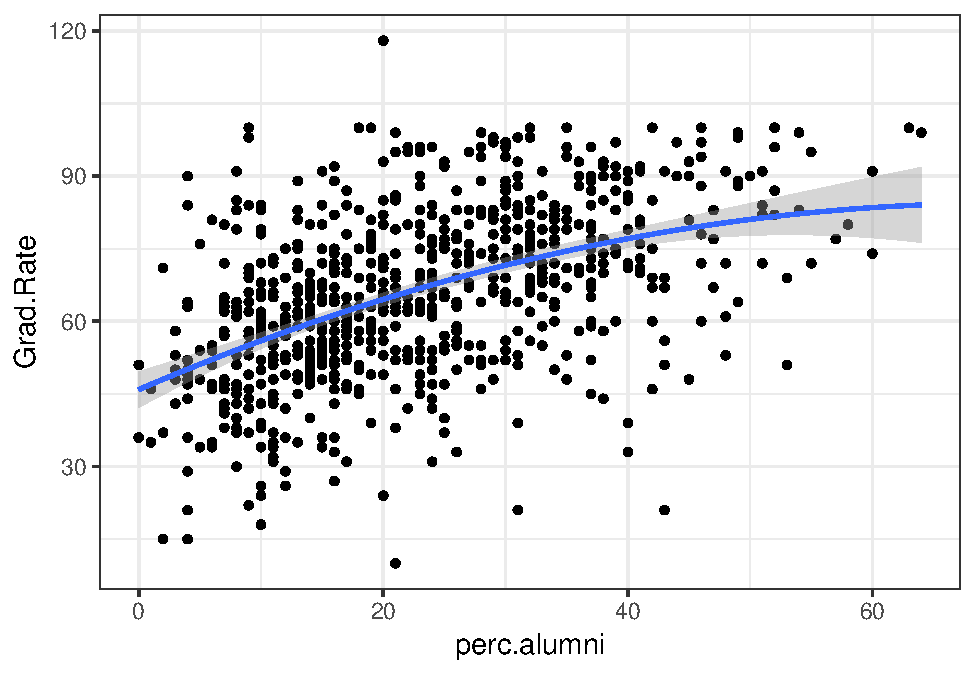
\includegraphics{Modelos_Estatisticos-2024-08-10_files/figure-latex/unnamed-chunk-24-1.pdf}

\begin{Shaded}
\begin{Highlighting}[]
\DocumentationTok{\#\#\# Extraindo os intervalos de confiança (95\%) para os parâmetros}
\FunctionTok{confint}\NormalTok{(ajuste2)}
\end{Highlighting}
\end{Shaded}

\begin{verbatim}
##                       2.5 %       97.5 %
## (Intercept)      42.2100816 49.582406847
## perc.alumni       0.7804723  1.391423440
## I(perc.alumni^2) -0.0131900 -0.002113503
\end{verbatim}

\subsection{Intervalo de confiança para a resposta média e para uma
predição}\label{intervalo-de-confianuxe7a-para-a-resposta-muxe9dia-e-para-uma-prediuxe7uxe3o}

Considere interesse em estimar a resposta \textbf{média} em um ponto
\(x′_0 = (1, x_{01], x_{02}, ..., x_{0k})\), ou seja, \(E (y |x_0)\).

A estimativa pontual é dada pelo valor ajustado pelo modelo em \(x_0\):
\[
\widehat{E(y|x_0)} = \hat{y_0} = x′_0 \hat{\beta}
\] O estimador apresentado é não viciado para a real resposta média, com
variância:

\[
Var(\widehat{E(y|x_0)}) = x'_0 Var(\hat{\beta})x_0
\] {[}73{]}

Um intervalo de confiança 100(1 − α)\% para a resposta média em x′ 0 =
(1, x01, x02, \ldots, x0k ) é dado por: \E (y \textbar x0) ± tn−p,α/2 ×
√ x′ 0 \Var ( ˆβ)x0. Considere agora que se deseja predizer a resposta
em um ponto (novo indivíduo) x′ 0 = (1, x01, x02, \ldots, x0k ). A
estimativa pontual, novamente, é dada pelo valor ajustado de y em x′ 0:
ˆy0 = x′ 0 ˆβ.

{[}74{]}

Neste caso, a variância de ˆy0 fica dada por: Var (ˆy0) = σ2 + x′ 0Var (
ˆβ)x0. Um intervalo de confiança 100(1 − α)\% para a predição de uma
nova observação em x0 fica dada por: ˆy0 ± tn−p,α/2 × √ ˆσ2 + x′ 0
\Var ( ˆβ)x0, em que ˆσ2 = QMRes .

\begin{Shaded}
\begin{Highlighting}[]
\DocumentationTok{\#\#\# vamos realizar algumas predições. Considere faculdades com os seguintes percentuais de ex{-}alunos contribuintes: 13, 28 e 45}

\NormalTok{new\_data }\OtherTok{\textless{}{-}} \FunctionTok{data.frame}\NormalTok{(}\AttributeTok{perc.alumni =} \FunctionTok{c}\NormalTok{(}\DecValTok{13}\NormalTok{,}\DecValTok{28}\NormalTok{,}\DecValTok{45}\NormalTok{))}
\FunctionTok{predict}\NormalTok{(ajuste2, }\AttributeTok{newdata =}\NormalTok{ new\_data, }\AttributeTok{se.fit =} \ConstantTok{TRUE}\NormalTok{)}
\end{Highlighting}
\end{Shaded}

\begin{verbatim}
## $fit
##        1        2        3 
## 58.72042 70.30381 79.26910 
## 
## $se.fit
##         1         2         3 
## 0.6820636 0.7449543 1.2061247 
## 
## $df
## [1] 774
## 
## $residual.scale
## [1] 14.91414
\end{verbatim}

\begin{Shaded}
\begin{Highlighting}[]
\DocumentationTok{\#\#\# Estimativas pontuais e erros padrões (nota: erros padrões para a resposta média)}
\end{Highlighting}
\end{Shaded}

\begin{Shaded}
\begin{Highlighting}[]
\FunctionTok{predict}\NormalTok{(ajuste2, }\AttributeTok{newdata =}\NormalTok{ new\_data, }\AttributeTok{interval =} \StringTok{\textquotesingle{}confidence\textquotesingle{}}\NormalTok{) }\CommentTok{\# para grupo com essa média}
\end{Highlighting}
\end{Shaded}

\begin{verbatim}
##        fit      lwr      upr
## 1 58.72042 57.38151 60.05933
## 2 70.30381 68.84144 71.76618
## 3 79.26910 76.90143 81.63676
\end{verbatim}

\begin{Shaded}
\begin{Highlighting}[]
\DocumentationTok{\#\#\# fit = estimando os formados a partir de um número de doadores (13,28,45). lwr e upr = limites do 95\% de confiaça.}

\DocumentationTok{\#\#\# Estimativas pontiais e intervalos de confiança (95\%) para a resposta **média**.}
\end{Highlighting}
\end{Shaded}

\begin{Shaded}
\begin{Highlighting}[]
\FunctionTok{predict}\NormalTok{(ajuste2, }\AttributeTok{newdata =}\NormalTok{ new\_data, }\AttributeTok{interval =} \StringTok{\textquotesingle{}prediction\textquotesingle{}}\NormalTok{) }\DocumentationTok{\#\# Para caso isolado (observação única)}
\end{Highlighting}
\end{Shaded}

\begin{verbatim}
##        fit      lwr       upr
## 1 58.72042 29.41286  88.02798
## 2 70.30381 40.99035  99.61727
## 3 79.26910 49.89656 108.64164
\end{verbatim}

\begin{Shaded}
\begin{Highlighting}[]
\DocumentationTok{\#\#\# fit = estimando os formados a partir de um número de doadores (13,28,45). lwr e upr = limites do 95\% de confiaça}

\DocumentationTok{\#\#\# Estimativas pontiais e intervalos de confiança (95\%) para a predição de **uma nova observação**.}
\end{Highlighting}
\end{Shaded}

\begin{Shaded}
\begin{Highlighting}[]
\DocumentationTok{\#\#\# Vamos plotar as bandas de confiança e predição. Para isso, vamos preparar uma base de dados com os valores ajustados e os ICs(95\%) para a resposta média e para as predições.}

\NormalTok{pred\_int }\OtherTok{\textless{}{-}} \FunctionTok{predict}\NormalTok{(ajuste2, }\AttributeTok{interval=}\StringTok{"prediction"}\NormalTok{)}
\NormalTok{med\_int }\OtherTok{\textless{}{-}} \FunctionTok{predict}\NormalTok{(ajuste2, }\AttributeTok{interval=}\StringTok{"confidence"}\NormalTok{)}
\NormalTok{data\_pred }\OtherTok{\textless{}{-}} \FunctionTok{data.frame}\NormalTok{(}\AttributeTok{pred\_lwr =}\NormalTok{ pred\_int[,}\StringTok{\textquotesingle{}lwr\textquotesingle{}}\NormalTok{], }\AttributeTok{pred\_upr =}\NormalTok{ pred\_int[,}\StringTok{\textquotesingle{}upr\textquotesingle{}}\NormalTok{],}
                        \AttributeTok{med\_lwr =}\NormalTok{ med\_int[,}\StringTok{\textquotesingle{}lwr\textquotesingle{}}\NormalTok{], }\AttributeTok{med\_upr =}\NormalTok{ med\_int[,}\StringTok{\textquotesingle{}upr\textquotesingle{}}\NormalTok{],}
                        \AttributeTok{fit =}\NormalTok{ med\_int[,}\StringTok{\textquotesingle{}fit\textquotesingle{}}\NormalTok{], }\AttributeTok{perc.alumni =}\NormalTok{ College}\SpecialCharTok{$}\NormalTok{perc.alumni,}
                        \AttributeTok{Grad.Rate =}\NormalTok{ College}\SpecialCharTok{$}\NormalTok{Grad.Rate)}

\FunctionTok{ggplot}\NormalTok{(data\_pred, }\FunctionTok{aes}\NormalTok{(}\AttributeTok{x =}\NormalTok{ perc.alumni, }\AttributeTok{y =}\NormalTok{ Grad.Rate))}\SpecialCharTok{+}
    \FunctionTok{geom\_point}\NormalTok{() }\SpecialCharTok{+}
    \FunctionTok{geom\_line}\NormalTok{(}\FunctionTok{aes}\NormalTok{(}\AttributeTok{y=}\NormalTok{med\_lwr), }\AttributeTok{color =} \StringTok{"red"}\NormalTok{, }\AttributeTok{linetype =} \StringTok{"dashed"}\NormalTok{, }\AttributeTok{linewidth =} \FloatTok{1.25}\NormalTok{) }\SpecialCharTok{+}
    \FunctionTok{geom\_line}\NormalTok{(}\FunctionTok{aes}\NormalTok{(}\AttributeTok{y=}\NormalTok{med\_upr), }\AttributeTok{color =} \StringTok{"red"}\NormalTok{, }\AttributeTok{linetype =} \StringTok{"dashed"}\NormalTok{, }\AttributeTok{linewidth =} \FloatTok{1.25}\NormalTok{) }\SpecialCharTok{+}
    \FunctionTok{geom\_line}\NormalTok{(}\FunctionTok{aes}\NormalTok{(}\AttributeTok{y=}\NormalTok{pred\_lwr), }\AttributeTok{color =} \StringTok{"green"}\NormalTok{, }\AttributeTok{linetype =} \StringTok{"dashed"}\NormalTok{, }\AttributeTok{linewidth =} \FloatTok{1.25}\NormalTok{) }\SpecialCharTok{+}
    \FunctionTok{geom\_line}\NormalTok{(}\FunctionTok{aes}\NormalTok{(}\AttributeTok{y=}\NormalTok{pred\_upr), }\AttributeTok{color =} \StringTok{"green"}\NormalTok{, }\AttributeTok{linetype =} \StringTok{"dashed"}\NormalTok{, }\AttributeTok{linewidth =} \FloatTok{1.25}\NormalTok{) }\SpecialCharTok{+}
    \FunctionTok{geom\_line}\NormalTok{(}\FunctionTok{aes}\NormalTok{(}\AttributeTok{y=}\NormalTok{fit), }\AttributeTok{color =} \StringTok{"black"}\NormalTok{, }\AttributeTok{linetype =} \StringTok{"dashed"}\NormalTok{, }\AttributeTok{linewidth =} \FloatTok{1.25}\NormalTok{) }\SpecialCharTok{+}
    \FunctionTok{theme\_bw}\NormalTok{(}\AttributeTok{base\_size =} \DecValTok{14}\NormalTok{)}
\end{Highlighting}
\end{Shaded}

\begin{Shaded}
\begin{Highlighting}[]
\DocumentationTok{\#\#\# Diagnóstico do ajuste (análise de resíduos)}

\DocumentationTok{\#\#\# Vamos produzir alguns gráficos para os resíduos}

\NormalTok{fit\_aj2 }\OtherTok{\textless{}{-}} \FunctionTok{fitted}\NormalTok{(ajuste2) }\DocumentationTok{\#\#\# Vetor de valores ajustados}
\NormalTok{resid\_aj2 }\OtherTok{\textless{}{-}} \FunctionTok{rstandard}\NormalTok{(ajuste2) }\DocumentationTok{\#\#\# Vetor de resíduos padronizados}

\NormalTok{data\_fit }\OtherTok{\textless{}{-}} \FunctionTok{data.frame}\NormalTok{(}\AttributeTok{y =}\NormalTok{ College}\SpecialCharTok{$}\NormalTok{Grad.Rate, fit\_aj2, resid\_aj2)}

\FunctionTok{ggplot}\NormalTok{(data\_fit, }\FunctionTok{aes}\NormalTok{(}\AttributeTok{x=}\NormalTok{y, }\AttributeTok{y=}\NormalTok{fit\_aj2)) }\SpecialCharTok{+} \FunctionTok{geom\_point}\NormalTok{() }\SpecialCharTok{+} \FunctionTok{stat\_smooth}\NormalTok{(}\AttributeTok{method=}\StringTok{"lm"}\NormalTok{) }\SpecialCharTok{+}
    \FunctionTok{theme\_bw}\NormalTok{(}\AttributeTok{base\_size =} \DecValTok{14}\NormalTok{)}
\DocumentationTok{\#\#\# Gráfico de valores observados versus valores ajustados. }

\FunctionTok{ggplot}\NormalTok{(ajuste2, }\FunctionTok{aes}\NormalTok{(}\AttributeTok{x=}\NormalTok{fit\_aj2, }\AttributeTok{y=}\NormalTok{resid\_aj2)) }\SpecialCharTok{+} \FunctionTok{geom\_point}\NormalTok{() }\SpecialCharTok{+}
    \FunctionTok{stat\_smooth}\NormalTok{(}\AttributeTok{method=}\StringTok{"loess"}\NormalTok{) }\SpecialCharTok{+} \FunctionTok{geom\_hline}\NormalTok{(}\AttributeTok{yintercept=}\DecValTok{0}\NormalTok{, }\AttributeTok{col=}\StringTok{"red"}\NormalTok{, }\AttributeTok{linetype=}\StringTok{"dashed"}\NormalTok{) }\SpecialCharTok{+}
    \FunctionTok{theme\_bw}\NormalTok{(}\AttributeTok{base\_size =} \DecValTok{14}\NormalTok{) }\SpecialCharTok{+}
    \FunctionTok{xlab}\NormalTok{(}\StringTok{\textquotesingle{}Valores ajustados\textquotesingle{}}\NormalTok{) }\SpecialCharTok{+}
    \FunctionTok{ylab}\NormalTok{(}\StringTok{\textquotesingle{}Resíduos\textquotesingle{}}\NormalTok{)}
\DocumentationTok{\#\#\# Gráfico de resíduos versus valores ajustados}

\FunctionTok{qqPlot}\NormalTok{(ajuste2)}
\DocumentationTok{\#\#\# Gráfico quantil{-}quantil para os resíduos}
\end{Highlighting}
\end{Shaded}

\begin{Shaded}
\begin{Highlighting}[]
\DocumentationTok{\#\#\# Parte 2 {-} Regressão linear múltipla, incluindo todas as variáveis da base como explicativas (exceto a taxa de formação, que é a resposta)}

\NormalTok{ajuste\_p2 }\OtherTok{\textless{}{-}} \FunctionTok{lm}\NormalTok{(Grad.Rate }\SpecialCharTok{\textasciitilde{}}\NormalTok{., }\AttributeTok{data =}\NormalTok{ College)}
\DocumentationTok{\#\#\# Ajuste da regressão linear múltipla. A especificação "\textasciitilde{}." indica que}
\DocumentationTok{\#\#\# todas as demais variáveis da base devem ser incluídas como explicativas.}
\DocumentationTok{\#\#\# A título de ilustração, se quiséssemos ajustar um modelo apenas com as}
\DocumentationTok{\#\#\# variáveis "Private", "Apps" e "Accept":}
\FunctionTok{summary}\NormalTok{(ajuste\_p2) }
\end{Highlighting}
\end{Shaded}

\begin{verbatim}
## 
## Call:
## lm(formula = Grad.Rate ~ ., data = College)
## 
## Residuals:
##     Min      1Q  Median      3Q     Max 
## -53.897  -7.132  -0.292   7.213  54.056 
## 
## Coefficients:
##               Estimate Std. Error t value Pr(>|t|)    
## (Intercept) 33.8736716  4.8480858   6.987 6.15e-12 ***
## PrivateYes   3.3813758  1.6965147   1.993 0.046605 *  
## Apps         0.0012984  0.0004418   2.939 0.003390 ** 
## Accept      -0.0006961  0.0008627  -0.807 0.419995    
## Enroll       0.0021593  0.0023081   0.936 0.349814    
## Top10perc    0.0548964  0.0717587   0.765 0.444501    
## Top25perc    0.1351288  0.0549667   2.458 0.014179 *  
## F.Undergrad -0.0004712  0.0004008  -1.176 0.240138    
## P.Undergrad -0.0014836  0.0003902  -3.802 0.000155 ***
## Outstate     0.0010174  0.0002334   4.359 1.49e-05 ***
## Room.Board   0.0019143  0.0005908   3.240 0.001246 ** 
## Books       -0.0022205  0.0029168  -0.761 0.446739    
## Personal    -0.0016635  0.0007698  -2.161 0.031000 *  
## PhD          0.0872827  0.0568102   1.536 0.124859    
## Terminal    -0.0747023  0.0623172  -1.199 0.231002    
## S.F.Ratio    0.0758222  0.1593102   0.476 0.634254    
## perc.alumni  0.2793343  0.0491750   5.680 1.91e-08 ***
## Expend      -0.0004565  0.0001542  -2.961 0.003163 ** 
## ---
## Signif. codes:  0 '***' 0.001 '**' 0.01 '*' 0.05 '.' 0.1 ' ' 1
## 
## Residual standard error: 12.75 on 759 degrees of freedom
## Multiple R-squared:  0.4615, Adjusted R-squared:  0.4495 
## F-statistic: 38.27 on 17 and 759 DF,  p-value: < 2.2e-16
\end{verbatim}

\begin{Shaded}
\begin{Highlighting}[]
\NormalTok{ajuste\_p2 }\OtherTok{\textless{}{-}} \FunctionTok{lm}\NormalTok{(Grad.Rate }\SpecialCharTok{\textasciitilde{}}\NormalTok{.}\SpecialCharTok{{-}}\NormalTok{Top25perc, }\AttributeTok{data =}\NormalTok{ College)}

\DocumentationTok{\#\# Todas menos a top 25. pq o top 10 e top 25 "se sobrepoe"}
\DocumentationTok{\#\# "ajustado os efeitos das outras variaveis"}

\FunctionTok{summary}\NormalTok{(ajuste\_p2) }
\end{Highlighting}
\end{Shaded}

\begin{verbatim}
## 
## Call:
## lm(formula = Grad.Rate ~ . - Top25perc, data = College)
## 
## Residuals:
##     Min      1Q  Median      3Q     Max 
## -47.786  -7.120  -0.257   7.171  54.050 
## 
## Coefficients:
##               Estimate Std. Error t value Pr(>|t|)    
## (Intercept) 36.3495104  4.7580380   7.640 6.57e-14 ***
## PrivateYes   3.3824039  1.7021347   1.987 0.047264 *  
## Apps         0.0011831  0.0004407   2.685 0.007421 ** 
## Accept      -0.0003936  0.0008568  -0.459 0.646059    
## Enroll       0.0015802  0.0023036   0.686 0.492938    
## Top10perc    0.1951766  0.0436553   4.471 8.98e-06 ***
## F.Undergrad -0.0003934  0.0004009  -0.981 0.326837    
## P.Undergrad -0.0014830  0.0003915  -3.788 0.000164 ***
## Outstate     0.0010161  0.0002342   4.339 1.63e-05 ***
## Room.Board   0.0019288  0.0005927   3.254 0.001188 ** 
## Books       -0.0020595  0.0029258  -0.704 0.481692    
## Personal    -0.0016865  0.0007723  -2.184 0.029273 *  
## PhD          0.0876416  0.0569982   1.538 0.124558    
## Terminal    -0.0565580  0.0620836  -0.911 0.362585    
## S.F.Ratio    0.0725205  0.1598322   0.454 0.650153    
## perc.alumni  0.2896423  0.0491582   5.892 5.73e-09 ***
## Expend      -0.0005259  0.0001521  -3.459 0.000573 ***
## ---
## Signif. codes:  0 '***' 0.001 '**' 0.01 '*' 0.05 '.' 0.1 ' ' 1
## 
## Residual standard error: 12.79 on 760 degrees of freedom
## Multiple R-squared:  0.4573, Adjusted R-squared:  0.4458 
## F-statistic: 40.02 on 16 and 760 DF,  p-value: < 2.2e-16
\end{verbatim}

Exemplo de numero de comodos e area em preço do imovel. Em sepada os
dois são significantes. No modelo tudo junto ajutado a area é positiva e
os comodos são negativos (mais comodos numa mesma area, ou seja comodos
menores, menos preço).

\begin{Shaded}
\begin{Highlighting}[]
\NormalTok{ajuste\_p2 }\OtherTok{\textless{}{-}} \FunctionTok{lm}\NormalTok{(Grad.Rate }\SpecialCharTok{\textasciitilde{}}\NormalTok{ Expend, }\AttributeTok{data =}\NormalTok{ College)}

\DocumentationTok{\#\# Todas menos a top 25. pq o top 10 e top 25 "se sobrepoe"}
\DocumentationTok{\#\# "ajustado os efeitos das outras variaveis"}

\FunctionTok{summary}\NormalTok{(ajuste\_p2) }
\end{Highlighting}
\end{Shaded}

\begin{verbatim}
## 
## Call:
## lm(formula = Grad.Rate ~ Expend, data = College)
## 
## Residuals:
##     Min      1Q  Median      3Q     Max 
## -60.179 -10.275   0.238  10.377  55.058 
## 
## Coefficients:
##              Estimate Std. Error t value Pr(>|t|)    
## (Intercept) 5.306e+01  1.194e+00   44.42   <2e-16 ***
## Expend      1.284e-03  1.088e-04   11.80   <2e-16 ***
## ---
## Signif. codes:  0 '***' 0.001 '**' 0.01 '*' 0.05 '.' 0.1 ' ' 1
## 
## Residual standard error: 15.83 on 775 degrees of freedom
## Multiple R-squared:  0.1524, Adjusted R-squared:  0.1513 
## F-statistic: 139.3 on 1 and 775 DF,  p-value: < 2.2e-16
\end{verbatim}

\begin{Shaded}
\begin{Highlighting}[]
\NormalTok{ajuste\_p2\_ilustrativo }\OtherTok{\textless{}{-}} \FunctionTok{lm}\NormalTok{(Grad.Rate }\SpecialCharTok{\textasciitilde{}}\NormalTok{ Private }\SpecialCharTok{+}\NormalTok{ Apps }\SpecialCharTok{+}\NormalTok{ Accept, }\AttributeTok{data =}\NormalTok{ College)}

\FunctionTok{summary}\NormalTok{(ajuste\_p2\_ilustrativo) }
\end{Highlighting}
\end{Shaded}

\begin{verbatim}
## 
## Call:
## lm(formula = Grad.Rate ~ Private + Apps + Accept, data = College)
## 
## Residuals:
##     Min      1Q  Median      3Q     Max 
## -51.513  -8.856   0.228  10.516  50.053 
## 
## Coefficients:
##               Estimate Std. Error t value Pr(>|t|)    
## (Intercept) 48.5068491  1.4308933  33.900  < 2e-16 ***
## PrivateYes  17.7697914  1.3831646  12.847  < 2e-16 ***
## Apps         0.0030589  0.0004228   7.235 1.12e-12 ***
## Accept      -0.0025493  0.0006842  -3.726 0.000209 ***
## ---
## Signif. codes:  0 '***' 0.001 '**' 0.01 '*' 0.05 '.' 0.1 ' ' 1
## 
## Residual standard error: 15.09 on 773 degrees of freedom
## Multiple R-squared:  0.2316, Adjusted R-squared:  0.2287 
## F-statistic: 77.68 on 3 and 773 DF,  p-value: < 2.2e-16
\end{verbatim}

\begin{Shaded}
\begin{Highlighting}[]
\DocumentationTok{\#\#\# Resumo do ajuste. Observe as variáveis com efeito significativo e os respectivos sinais.}
\DocumentationTok{\#\#\# Variáveis com p{-}valor (Pr(\textgreater{}|t|)) \textless{} 0.05 podem ser consideradas com efeito }
\DocumentationTok{\#\#\# significativo na taxa de formados. Desta forma, as variáveis com efeito}
\DocumentationTok{\#\#\# significativo na taxa de formados são Private (Yes), Apps, Top25perc, Outstate,}
\DocumentationTok{\#\#\# Room.Board, 0.2793343; Já as variáveis com efeito negativo na taxa de formados}
\DocumentationTok{\#\#\# são P.Undergrad, Personal e Expend.}
\end{Highlighting}
\end{Shaded}

\begin{Shaded}
\begin{Highlighting}[]
\DocumentationTok{\#\#\# Apenas para fins de discussão, vamos ajustar um modelo de regressão tendo como}
\DocumentationTok{\#\#\# única variável explicativa o gasto por aluno.}
\NormalTok{ajuste\_temp }\OtherTok{\textless{}{-}} \FunctionTok{lm}\NormalTok{(Grad.Rate }\SpecialCharTok{\textasciitilde{}}\NormalTok{ Expend, }\AttributeTok{data =}\NormalTok{ College)}
\FunctionTok{summary}\NormalTok{(ajuste\_temp)}

\DocumentationTok{\#\#\# Compare o efeito do gasto por aluno na taxa de formação produzida pelo}
\DocumentationTok{\#\#\# modelo em que ajustamos também os efeitos das demais variáveis com o}
\DocumentationTok{\#\#\# efeito produzido pelo modelo em que as demais variáveis não são consideradas.}
\DocumentationTok{\#\#\# Qual a diferença? Como você a justifica?}
\end{Highlighting}
\end{Shaded}

\begin{Shaded}
\begin{Highlighting}[]
\FunctionTok{par}\NormalTok{(}\AttributeTok{mfrow =} \FunctionTok{c}\NormalTok{(}\DecValTok{2}\NormalTok{,}\DecValTok{2}\NormalTok{))}
\FunctionTok{plot}\NormalTok{(ajuste\_p2, }\AttributeTok{which =} \DecValTok{1}\SpecialCharTok{:}\DecValTok{4}\NormalTok{)}
\DocumentationTok{\#\#\# Gráficos de resíduos.}
\DocumentationTok{\#\#\# O gráfico do canto superior esquerdo indica que a variância dos resíduos varia}
\DocumentationTok{\#\#\# um pouco com a média (fitted values), e que os resíduos apresentam algum desvio}
\DocumentationTok{\#\#\# da normalidade (conforme o qqplot). Ainda, conforme o gráfico do canto inferior}
\DocumentationTok{\#\#\# direito, algumas observações podem ser identificadas como possivelmente influentes,}
\DocumentationTok{\#\#\# produzindo maiores valores para a distância de Cook.}

\DocumentationTok{\#\#\# Embora tenhamos alguns indicativos (ainda que não tão severos) de falta de ajuste}
\DocumentationTok{\#\#\# da regressão linear, para fins didáticos vamos seguir a análise com esse tipo}
\DocumentationTok{\#\#\# de modelagem.}
\end{Highlighting}
\end{Shaded}

\begin{Shaded}
\begin{Highlighting}[]
\DocumentationTok{\#\#\# Agora, vamos para a etapa de seleção de covariáveis. Para isso, vamos}
\DocumentationTok{\#\#\# usar os recursos do pacote leaps. Vamos consultar a documentação da função}
\DocumentationTok{\#\#\# regsubsets.}

\FunctionTok{help}\NormalTok{(}\StringTok{"regsubsets"}\NormalTok{)}

\NormalTok{all\_reg }\OtherTok{\textless{}{-}} \FunctionTok{regsubsets}\NormalTok{(Grad.Rate }\SpecialCharTok{\textasciitilde{}}\NormalTok{ ., }\AttributeTok{method =} \StringTok{"exhaustive"}\NormalTok{, }\AttributeTok{nvmax =} \DecValTok{18}\NormalTok{, }\AttributeTok{data =}\NormalTok{ College)}
\DocumentationTok{\#\#\# Explorando TODAS as regressões possíveis}
\NormalTok{all\_reg}
\end{Highlighting}
\end{Shaded}

\begin{Shaded}
\begin{Highlighting}[]
\FunctionTok{plot}\NormalTok{(all\_reg, }\AttributeTok{scale=}\StringTok{"r2"}\NormalTok{) }\DocumentationTok{\#\#\# Resultados baseados no R2}
\FunctionTok{plot}\NormalTok{(all\_reg, }\AttributeTok{scale=}\StringTok{"adjr2"}\NormalTok{) }\DocumentationTok{\#\#\# Resultados baseados no R2 ajustado}
\FunctionTok{plot}\NormalTok{(all\_reg, }\AttributeTok{scale=}\StringTok{"bic"}\NormalTok{) }\DocumentationTok{\#\#\# Resultados baseados no BIC}
\DocumentationTok{\#\#\# Nesses gráficos avaliamos os resultados dos critérios para os melhores}
\DocumentationTok{\#\#\# modelos ajustados com cada número de covariáveis.}

\NormalTok{s1 }\OtherTok{\textless{}{-}} \FunctionTok{summary}\NormalTok{(all\_reg, }\AttributeTok{matrix.logical=}\ConstantTok{TRUE}\NormalTok{)}
\NormalTok{s1 }\DocumentationTok{\#\#\# A matriz lógica permite identificar as covariáveis selecionadas }
\DocumentationTok{\#\#\# em cada modelo.}

\NormalTok{s1}\SpecialCharTok{$}\NormalTok{rsq }\DocumentationTok{\#\#\# Valores de R2 para cada um dos modelos selecionados}
\NormalTok{s1}\SpecialCharTok{$}\NormalTok{adjr2 }\DocumentationTok{\#\#\# Valores de R2 ajustado para cada um dos modelos selecionados}
\NormalTok{s1}\SpecialCharTok{$}\NormalTok{bic }\DocumentationTok{\#\#\# Valores de BIC para cada um dos modelos selecionados}

\FunctionTok{which.max}\NormalTok{(s1}\SpecialCharTok{$}\NormalTok{adjr2)}
\FunctionTok{coef}\NormalTok{(all\_reg, }\AttributeTok{id =} \DecValTok{12}\NormalTok{)}
\DocumentationTok{\#\#\# O modelo com doze covariáveis produziu maior valor de R2 ajustado.}

\FunctionTok{which.min}\NormalTok{(s1}\SpecialCharTok{$}\NormalTok{bic) }
\FunctionTok{coef}\NormalTok{(all\_reg, }\AttributeTok{id =} \DecValTok{7}\NormalTok{)}
\DocumentationTok{\#\#\# O modelo com sete covariáveis produziu menor valor de BIC.}

\FunctionTok{which.max}\NormalTok{(s1}\SpecialCharTok{$}\NormalTok{rsq) }
\FunctionTok{coef}\NormalTok{(all\_reg, }\AttributeTok{id =} \DecValTok{17}\NormalTok{)}
\DocumentationTok{\#\#\# O modelo com 17 covariáveis produziu menor valor de R2 (obviamente).}

\DocumentationTok{\#\#\# Vamos produzir alguns gráficos usando os resultados desta análise.}
\NormalTok{n\_cov }\OtherTok{\textless{}{-}} \DecValTok{1}\SpecialCharTok{:}\DecValTok{17}

\FunctionTok{plot}\NormalTok{(n\_cov, s1}\SpecialCharTok{$}\NormalTok{bic, }\AttributeTok{type =} \StringTok{\textquotesingle{}b\textquotesingle{}}\NormalTok{, }\AttributeTok{xlab =} \StringTok{\textquotesingle{}Número de covariáveis\textquotesingle{}}\NormalTok{, }
     \AttributeTok{ylab =} \StringTok{\textquotesingle{}BIC\textquotesingle{}}\NormalTok{, }\AttributeTok{las =} \DecValTok{1}\NormalTok{, }\AttributeTok{pch =} \DecValTok{20}\NormalTok{)}
\FunctionTok{axis}\NormalTok{(}\DecValTok{1}\NormalTok{,}\DecValTok{1}\SpecialCharTok{:}\DecValTok{17}\NormalTok{)}

\FunctionTok{plot}\NormalTok{(n\_cov, s1}\SpecialCharTok{$}\NormalTok{adjr2, }\AttributeTok{type =} \StringTok{\textquotesingle{}b\textquotesingle{}}\NormalTok{, }\AttributeTok{xlab =} \StringTok{\textquotesingle{}Número de covariáveis\textquotesingle{}}\NormalTok{, }
     \AttributeTok{ylab =} \StringTok{\textquotesingle{}Adjusted R2\textquotesingle{}}\NormalTok{, }\AttributeTok{las =} \DecValTok{1}\NormalTok{, }\AttributeTok{pch =} \DecValTok{20}\NormalTok{)}
\FunctionTok{axis}\NormalTok{(}\DecValTok{1}\NormalTok{,}\DecValTok{1}\SpecialCharTok{:}\DecValTok{17}\NormalTok{)}

\FunctionTok{plot}\NormalTok{(n\_cov, s1}\SpecialCharTok{$}\NormalTok{rsq, }\AttributeTok{type =} \StringTok{\textquotesingle{}b\textquotesingle{}}\NormalTok{, }\AttributeTok{xlab =} \StringTok{\textquotesingle{}Número de covariáveis\textquotesingle{}}\NormalTok{, }
     \AttributeTok{ylab =} \StringTok{\textquotesingle{}R2\textquotesingle{}}\NormalTok{, }\AttributeTok{las =} \DecValTok{1}\NormalTok{, }\AttributeTok{pch =} \DecValTok{20}\NormalTok{)}
\FunctionTok{axis}\NormalTok{(}\DecValTok{1}\NormalTok{,}\DecValTok{1}\SpecialCharTok{:}\DecValTok{17}\NormalTok{)}


\DocumentationTok{\#\#\# Para finalizar, vamos aplicar os algoritmos de seleção do tipo}
\DocumentationTok{\#\#\# stepwise. Primeiramente fixando k = 2, estamos definindo o AIC como critério de}
\DocumentationTok{\#\#\# seleção, temos:}

\DocumentationTok{\#\#\# Método backward}
\NormalTok{step\_back\_AIC }\OtherTok{\textless{}{-}} \FunctionTok{step}\NormalTok{(aj\_full, }\AttributeTok{direction =} \StringTok{"backward"}\NormalTok{, }\AttributeTok{data =}\NormalTok{ College, }\AttributeTok{k =} \DecValTok{2}\NormalTok{)}
\FunctionTok{summary}\NormalTok{(step\_back\_AIC)}

\DocumentationTok{\#\#\# Método forward. Para o método forward devemos definir o escopo da seleção}
\DocumentationTok{\#\#\# (menor e maior modelo). O menor seria o modelo nulo (apenas com o intercepto),}
\DocumentationTok{\#\#\# enquanto o maior seria o modelo com todas as covariáveis.}
\NormalTok{aj\_lower }\OtherTok{\textless{}{-}} \FunctionTok{lm}\NormalTok{(Grad.Rate}\SpecialCharTok{\textasciitilde{}}\DecValTok{1}\NormalTok{, }\AttributeTok{data =}\NormalTok{ College)}

\NormalTok{aj\_upper }\OtherTok{\textless{}{-}} \FunctionTok{lm}\NormalTok{(Grad.Rate}\SpecialCharTok{\textasciitilde{}}\NormalTok{., }\AttributeTok{data =}\NormalTok{ College)}
\FunctionTok{formula}\NormalTok{(aj\_upper)}

\NormalTok{step\_for\_AIC }\OtherTok{\textless{}{-}} \FunctionTok{step}\NormalTok{(aj\_lower, }\AttributeTok{direction =} \StringTok{"forward"}\NormalTok{, }\AttributeTok{scope=}\FunctionTok{formula}\NormalTok{(aj\_upper), }
                     \AttributeTok{data =}\NormalTok{ College, }\AttributeTok{k =} \DecValTok{2}\NormalTok{)}
\FunctionTok{summary}\NormalTok{(step\_for\_AIC)}

\DocumentationTok{\#\#\# Finalmente, o algoritmo que considera tanto exclusão quanto inclusão de}
\DocumentationTok{\#\#\# covariáveis a cada passo}
\NormalTok{step\_both\_AIC }\OtherTok{\textless{}{-}} \FunctionTok{step}\NormalTok{(aj\_full, }\AttributeTok{direction =} \StringTok{"both"}\NormalTok{, }\AttributeTok{data =}\NormalTok{ College, }\AttributeTok{k =} \DecValTok{2}\NormalTok{)}
\FunctionTok{summary}\NormalTok{(step\_both\_AIC)}

\DocumentationTok{\#\#\# Vamos comparar os ajustes.}
\FunctionTok{data.frame}\NormalTok{(}\FunctionTok{compareCoefs}\NormalTok{(step\_back\_AIC, step\_for\_AIC, step\_both\_AIC))}


\DocumentationTok{\#\#\# Agora fixando k = log(n) (critério BIC):}

\DocumentationTok{\#\#\# Método backward}
\NormalTok{step\_back\_BIC }\OtherTok{\textless{}{-}} \FunctionTok{step}\NormalTok{(aj\_full, }\AttributeTok{direction =} \StringTok{"backward"}\NormalTok{, }\AttributeTok{data =}\NormalTok{ College, }\AttributeTok{k =} \FunctionTok{log}\NormalTok{(}\FunctionTok{nrow}\NormalTok{(College)))}
\FunctionTok{summary}\NormalTok{(step\_back\_BIC)}

\DocumentationTok{\#\#\# Método forward. Para o método forward devemos definir o escopo da seleção}
\DocumentationTok{\#\#\# (menor e maior modelo). O menor seria o modelo nulo (apenas com o intercepto),}
\DocumentationTok{\#\#\# enquanto o maior seria o modelo com todas as covariáveis.}
\NormalTok{aj\_lower }\OtherTok{\textless{}{-}} \FunctionTok{lm}\NormalTok{(Grad.Rate}\SpecialCharTok{\textasciitilde{}}\DecValTok{1}\NormalTok{, }\AttributeTok{data =}\NormalTok{ College)}

\NormalTok{aj\_upper }\OtherTok{\textless{}{-}} \FunctionTok{lm}\NormalTok{(Grad.Rate}\SpecialCharTok{\textasciitilde{}}\NormalTok{., }\AttributeTok{data =}\NormalTok{ College)}
\FunctionTok{formula}\NormalTok{(aj\_upper)}

\NormalTok{step\_for\_BIC }\OtherTok{\textless{}{-}} \FunctionTok{step}\NormalTok{(aj\_lower, }\AttributeTok{direction =} \StringTok{"forward"}\NormalTok{, }\AttributeTok{scope=}\FunctionTok{formula}\NormalTok{(aj\_upper), }
                     \AttributeTok{data =}\NormalTok{ College, }\AttributeTok{k =} \FunctionTok{log}\NormalTok{(}\FunctionTok{nrow}\NormalTok{(College)))}
\FunctionTok{summary}\NormalTok{(step\_for\_BIC)}

\DocumentationTok{\#\#\# Finalmente, o algoritmo que considera tanto exclusão quanto inclusão de}
\DocumentationTok{\#\#\# covariáveis a cada passo}
\NormalTok{step\_both\_BIC }\OtherTok{\textless{}{-}} \FunctionTok{step}\NormalTok{(aj\_full, }\AttributeTok{direction =} \StringTok{"both"}\NormalTok{, }\AttributeTok{data =}\NormalTok{ College, }\AttributeTok{k =} \FunctionTok{log}\NormalTok{(}\FunctionTok{nrow}\NormalTok{(College)))}
\FunctionTok{summary}\NormalTok{(step\_both\_BIC)}

\DocumentationTok{\#\#\# Vamos comparar os ajustes.}
\FunctionTok{data.frame}\NormalTok{(}\FunctionTok{compareCoefs}\NormalTok{(step\_back\_BIC, step\_for\_BIC, step\_both\_BIC))}
\end{Highlighting}
\end{Shaded}

\subsection{Seleção de variáveis
explicativas}\label{seleuxe7uxe3o-de-variuxe1veis-explicativas}

Princípio de Occam: Dentre as várias explicações possíveis para um
fenômeno, a mais simples é a melhor

Fuechsel, técnico da IBM: Garbage in, garbage out

\begin{itemize}
\tightlist
\item
  Neste módulo vamos tratar da seleção de covariáveis para o ajuste de
  modelos de regressão linear.
\item
  O objetivo é identificar um modelo parcimonioso, capaz de proporcionar
  bom ajuste com a menor quantidade possível de parâmetros.
\item
  Diferentes métodos podem ser aplicados na seleção de um subconjunto
  ``ótimo'' de variáveis.
\item
  Importante ter em mente que diferentes métodos de seleção,
  frequentemente, remetem a modelos distintos (lembre-se: ``All models
  are wrong but some are useful'')
\end{itemize}

\subsubsection{Por que não incluir todas as covariáveis no
modelo?}\label{por-que-nuxe3o-incluir-todas-as-covariuxe1veis-no-modelo}

1 Um dos objetivos principais da análise de regressão é explicar a
relação entre as variáveis de maneira simples e interpretável; 2 Quanto
maior o número de parâmetros no modelo, menos graus de liberdade para os
resíduos, menor precisão para as inferências; 3 Quanto maior o número de
variáveis incluídas no modelo, maior a possibilidade de
multicolinearidade; 4 Quanto mais complexo (parametrizado) o modelo,
melhor o ajuste da amostra, mas menor seu poder de generalização (baixo
poder preditivo)

\subsubsection{Como proceder a seleção do
modelo?}\label{como-proceder-a-seleuxe7uxe3o-do-modelo}

Antes de aplicar qualquer método analítico para seleção de covariáveis,
é conveniente fazer uma pré-triagem de variáveis, buscando eliminar
variáveis que, a título de exemplo: - Sejam redundantes; - Apresentem
elevado erro de medida; - Não estejam no contexto do estudo; -
Apresentem elevada taxa de dados missing. . .

\subsubsection{Critérios para avaliação e comparação de
modelos}\label{crituxe9rios-para-avaliauxe7uxe3o-e-comparauxe7uxe3o-de-modelos}

\begin{itemize}
\tightlist
\item
  No processo de seleção de covariáveis, diferentes critérios podem ser
  usados para comparar os modelos produzidos. Alguns deles são descritos
  na sequência.
\item
  \textbf{Coeficiente de deteminação} (\(R^2\)) - O coeficiente de
  determinação corresponde à proporção da variação dos dados explicada
  pela regressão:
\end{itemize}

\[
R^2 = \frac{SQ_{Total}-SQ_{R}^{es}}{SQ_{total}} = 1 = \frac{SQ_{Res}}{SQ_{total}}
\]

em que

\[
SQ_{Total} = \sum^n_{i-1}{(y_i - \overline{y})^2} \space \space e \space \space SQ_{Res} = \sum^n_{i-1}{(y_i - \hat{y}_i)^2}
\]

são as somas de quadrados total e atribuída aos resíduos,
respectivamente

\begin{Shaded}
\begin{Highlighting}[]
\FunctionTok{summary}\NormalTok{(ajuste22)}
\end{Highlighting}
\end{Shaded}

\begin{verbatim}
## 
## Call:
## lm(formula = Grad.Rate ~ ., data = College)
## 
## Residuals:
##     Min      1Q  Median      3Q     Max 
## -53.897  -7.132  -0.292   7.213  54.056 
## 
## Coefficients:
##               Estimate Std. Error t value Pr(>|t|)    
## (Intercept) 33.8736716  4.8480858   6.987 6.15e-12 ***
## PrivateYes   3.3813758  1.6965147   1.993 0.046605 *  
## Apps         0.0012984  0.0004418   2.939 0.003390 ** 
## Accept      -0.0006961  0.0008627  -0.807 0.419995    
## Enroll       0.0021593  0.0023081   0.936 0.349814    
## Top10perc    0.0548964  0.0717587   0.765 0.444501    
## Top25perc    0.1351288  0.0549667   2.458 0.014179 *  
## F.Undergrad -0.0004712  0.0004008  -1.176 0.240138    
## P.Undergrad -0.0014836  0.0003902  -3.802 0.000155 ***
## Outstate     0.0010174  0.0002334   4.359 1.49e-05 ***
## Room.Board   0.0019143  0.0005908   3.240 0.001246 ** 
## Books       -0.0022205  0.0029168  -0.761 0.446739    
## Personal    -0.0016635  0.0007698  -2.161 0.031000 *  
## PhD          0.0872827  0.0568102   1.536 0.124859    
## Terminal    -0.0747023  0.0623172  -1.199 0.231002    
## S.F.Ratio    0.0758222  0.1593102   0.476 0.634254    
## perc.alumni  0.2793343  0.0491750   5.680 1.91e-08 ***
## Expend      -0.0004565  0.0001542  -2.961 0.003163 ** 
## ---
## Signif. codes:  0 '***' 0.001 '**' 0.01 '*' 0.05 '.' 0.1 ' ' 1
## 
## Residual standard error: 12.75 on 759 degrees of freedom
## Multiple R-squared:  0.4615, Adjusted R-squared:  0.4495 
## F-statistic: 38.27 on 17 and 759 DF,  p-value: < 2.2e-16
\end{verbatim}

\textbf{Multiple R-squared: 0.4615}

\subsubsection{Critérios para avaliação e comparação de
modelos}\label{crituxe9rios-para-avaliauxe7uxe3o-e-comparauxe7uxe3o-de-modelos-1}

\begin{itemize}
\item
  O coeficiente de determinação expressa a proporção da variabilidade
  total explicada pelo modelo ajustado.
\item
  O valor de \(R^2\) nunca decresce à medida que novas covariáveis são
  incluídas no modelo.
\item
  Assim, não se deve optar pela seleção do modelo que produz maior
  \(R^2\), pois esse modelo incluiria, necessariamente, o maior número
  possível de covariáveis.
\item
  \textbf{Coeficiente de deteminação ajustado} - O coeficiente de
  determinação ajustado (ou simplesmente \(R^2\) ajustado) é definido
  por:
\end{itemize}

\[
R_{Aj}^2 = 1 - (\frac{n-1}{n-p}) (1 - R^2)
\]

em que n e p são o número de observações e o número de parâmetros do
modelo.

\begin{itemize}
\tightlist
\item
  Diferentemente do que ocorre para \(R_2\), o valor de \(R_{Aj}^2\)
  pode não aumentar mediante inclusão de novas variáveis ao modelo.
  Deve-se optar por modelos com maiores valores de \(R_{Aj}^2\).
\end{itemize}

\paragraph{Akaike Information Criterion
(AIC)}\label{akaike-information-criterion-aic}

\begin{itemize}
\tightlist
\item
  O critério de informação de Akaike (Akaike Information Criterion), ou
  simplesmente AIC, é definido por: \[
  AIC = -2l(\hat{\theta}) + 2p
  \]
\end{itemize}

em que \(l(\hat{\theta})\) é a log-verossimilhança maximizada do modelo
(calculada com base nos emv's dos parâmetros) e p o número de parâmetros
do modelo.

\begin{itemize}
\tightlist
\item
  O AIC pode ser usado para qualquer modelo ajustado por máxima
  verossimilhança. No caso de um modelo de regressão linear temos:
\end{itemize}

\[
AIC = −n \space ln(SQ_{Res} /n) + 2p.
\] - O componente 2p, na expressão do AIC , atua como termo de
penalização atribuído à complexidade (número de parâmetros) do modelo.

\paragraph{Critério de Informação Bayesiano
(BIC)}\label{crituxe9rio-de-informauxe7uxe3o-bayesiano-bic}

\begin{itemize}
\tightlist
\item
  Um critério alternativo ao AIC é o Critério de Informação Bayesiano
  (BIC), definido, para um modelo de regressão linear, por:
\end{itemize}

\[
BIC = −n \space ln(SQ_{Res} /n) + ln(n)p 
\]

\begin{itemize}
\tightlist
\item
  O BIC penaliza mais fortemente a complexidade do modelo que o AIC ao
  substituir p por \(ln(n)\) como fator de penalização.
\item
  Devemos selecionar modelos com menores valores de AIC (ou BIC).
\end{itemize}

\subsection{Seleção de modelos baseada em critérios de qualidade de
ajuste}\label{seleuxe7uxe3o-de-modelos-baseada-em-crituxe9rios-de-qualidade-de-ajuste}

\begin{itemize}
\item
  Um primeiro algoritmo de seleção de modelos, baseados em critérios de
  qualidade de ajuste, é o método \textbf{todas as regressões
  possíveis};
\item
  Suponha uma análise de regressão com k variáveis;
\item
  Uma primeira alternativa consiste em ajustar todos os possíveis
  modelos de regressão com \(j \le k\) covariáveis, para
  \(j = 0, 1, 2, ..., k\);
\item
  Para cada modelo de regressão ajustado calcula-se o valor do critério
  de seleção escolhido \((AIC, BIC \space ou \space R_{Aj}^2 . . . )\);
\item
  O modelo selecionado será quele que apresentar o valor ótimo para o
  critério adotado (maior \(R_{Aj}^2\), menor AIC,. . . ).
\item
  O método baseado em todas as regressões possíveis torna-se inviável
  mesmo para um número moderado de covariáveis;
\item
  Para k variáveis o número de regressões possíveis é \(2^k\) . Para k =
  30, por exemplo, teríamos \(1.073.741.824\) modelos possíveis!
\item
  Como alternativa ao método de todas as regressões possíveis podemos
  usar os algoritmos backward, forward ou stepwise substituindo o teste
  F por algum dos critérios apresentado
\end{itemize}

\subsubsection{Seleção de covariáveis - Método
backward}\label{seleuxe7uxe3o-de-covariuxe1veis---muxe9todo-backward}

\begin{enumerate}
\def\labelenumi{\arabic{enumi}.}
\tightlist
\item
  Ajuste o modelo de regressão com todas as k covariáveis disponíveis;
  2.Remova uma a uma as covariáveis do modelo e calcule o valor do
  critério de qualidade de ajuste adotado (digamos o AIC, para
  ilustração);
\item
  Remova do modelo (em definitivo) a variável cuja exclusão resultar em
  menor AIC;
\item
  Os passos 1 a 3 são repetidos para o novo modelo (com a remoção da
  covariável) e o processo continua até o momento em que nenhuma remoção
  produzir um ajuste com menor AIC
\end{enumerate}

\subsubsection{Seleção de covariáveis - Método
forward}\label{seleuxe7uxe3o-de-covariuxe1veis---muxe9todo-forward}

\begin{enumerate}
\def\labelenumi{\arabic{enumi}.}
\tightlist
\item
  Ajuste o modelo nulo (sem covariáveis);
\item
  Adicione uma a uma as covariáveis ao modelo e calcule o valor do
  critério de qualidade de ajuste adotado (digamos o AIC, para
  ilustração);
\item
  Inclua no modelo (em definitivo) a variável cuja exclusão resultar em
  menor AIC;
\item
  Os passos 1 a 3 são repetidos para o novo modelo (com a inclusão da
  covariável) e o processo continua até o momento em que nenhuma
  inclusão produzir um ajuste com menor AIC
\end{enumerate}

\subsubsection{Seleção de covariáveis - Método
combinado}\label{seleuxe7uxe3o-de-covariuxe1veis---muxe9todo-combinado}

\begin{enumerate}
\def\labelenumi{\arabic{enumi}.}
\tightlist
\item
  Ajuste o modelo de regressão com todas as k covariáveis disponíveis.
  Proceda como descrito no algoritmo backward, mas. . .
\item
  A cada passo do algoritmo, avalie uma a uma tanto a inclusão das
  variáveis não inseridas quanto a exclusão das variáveis que compõem o
  modelo.
\item
  Inclua (exclua) no modelo a variável cuja inclusão (exclusão) resultar
  em menor AIC;
\item
  Os passos 1 a 3 são repetidos para o novo modelo (com a inclusão
  (exclusão) da covariável) e o processo continua até o momento em que
  nenhuma inclusão (ou exclusão) produzir um ajuste com menor AIC.
\end{enumerate}

\end{document}
